\begin{refsegment}

\chapter[Genealogies in multitype regulated branching particle models]{Genealogies in multitype regulated branching particle models}\label{chp4_multitype}
\chaptermark{Genealogies in multitype regulated branching particle models}

\objectif{This chapter extends the methodology developped in Chapter~\ref{chp3_singletype}. It aims to provide a comprehensive recursive formula to grasp the distribution of the genealogies of any population model as a function of the contributions of the stochastic neutral fractions through a positive semigroup.
The strength of our approach is that this semigroup can be defined for any model of population, making the formula quite general and of intrinsic value.
As a first application of our methodology, we study a broad class of frequency-dependent individual-based models on a finite type space, which is a multitype version of the work in Chapter~\ref{chp3_singletype} \citep{AFRS_2025}. Under a second moment assumption, we close the induction and  prove that the limiting distribution of the genealogies is given by the Kingman coalescent.
 The underlying structure only influences the effective population size, hence the genetic diversity of the population.
}


\section{Preliminaries}

In what follows, the notation $C_1$, $C_2$, \textit{etc.} will refer to constants appearing inside proofs and which do not need to be specified -- the same notation may be used several times for different constants.

\subsection{Motivation and related literature}

\paragraph{Forward and backward approaches to the genealogies of a population.}
Neutral fractions were introduced by~\cite{hallatschek_gene_2008} for populations described by a reaction-diffusion system, typically governed by a stochastic differential equation such as the Fisher-KPP equation.
They consist in subdividing of the population into subfamilies who all share the same dynamic (hence the term ``neutral'') and are a very natural tool to study the diversity of a population.
Tracking the progeny of subfamilies can be seen as tracking the evolution of an allele without selective advantage or disadvantage.
The evolution of the neutral markers is a way to study the evolution of diversity due to genetic drift.  

Instead of tracking allele frequencies forward in time, we can study the ancestral lineages traced back from some individuals uniformly picked in the population at some fixed time. We note that in this article we will always consider sampling at a fixed ``present time'', even when this is not specified. This backward-in-time approach is called coalescent theory. The shape of the genealogies determines how many mutations we see and how frequent they are. Long branches imply more diversity, while shallow branching points imply that many individuals share a recent common ancestor, which in turn means that there is low diversity in the population. Knowing the shape of the genealogies gives a prediction of neutral allele frequencies, as has been shown in some heuristics. For some models, duality formulas connect the forward in time population process and allele frequency dynamics to the ancestral coalescent process. Some textbook examples of population processes for which duality has been thoroughly studied include the Wright--Fisher model, the Moran model, the spatial Fleming--Viot process, see~\cite{carinci_dualities_2015}. 
However, to the best of our knowledge, there is no general method allowing us to deduce the formal distribution of the coalescent directly from the forward-in-time dynamics. For most models, as highlighted in~\cite{Julie_Zsofia}, it remains a technical challenge.

\paragraph{Coalescent theory in regulated and structured populations models.} 
Not much is known about the genealogies of individual-based models, except in some very particular cases in which dualities can be established between the forward and backward dynamics.
On one side are branching population models, such as the multitype Galton--Watson process, or spatially structured models such as the one studied by~\cite{julie_tourniaire_branching_2024}. In these models, there are no interactions, individuals reproduce and move in space independently. 
In the critical multitype Galton--Watson process, it is well-known that conditional upon survival, the population grows linearly (by the so-called Yaglom's theorem from~\cite{kesten_galton-watson_1966}) and that the genealogy from uniform sampling at present converges to that of a Feller diffusion~\citep{7_authors_paper}.
This coalescing object is a  Kingman coalescent time-changed by the (random) population size and called the Brownian Coalescent Point Process (shortened CPP). It is the ultrametric version of the celebrated Continuum Random Tree of~\cite{aldous_continuum_1991}. 
The genealogy of the particle model of~\cite{julie_tourniaire_branching_2024} was proved in the fully pushed regime to converge to the Brownian CPP by~\cite{schertzer2023spectral} and in the semi-pushed regime to the genealogy of an $\alpha$-stable CSBP (stable CPP) by~\cite{foutel-rodier_convergence_2024}. 
All of these results use a moment-based methodology to derive convergence of the genealogies.

On the other side of the spectrum are purely conservative population models, such as the Moran model, the Wright--Fisher model, or more generally the class of excheangeable Cannings models. In these models, there is no demography: the population size is fixed and reproduction events of individuals are anti-correlated. The genealogies of these models are well-known to converge to the $\Lambda$-coalescents of~\cite{Pitman:1999aa} and~\cite{sagitov1999general} in the large population limit. Because these coalescent models are extensively documented in the literature, they have become widely used in population genetics and phylogenetics to reconstruct evolutionary paths, and analyze the genetic diversity of populations. In particular, the binary Kingman coalescent of~\cite{Kingman:1982aa} serves as a baseline model for panmictic and neutral populations.
More specifically, when the variance of the offspring distribution rescaled by the population size $K$ has a finite limit as $K \to \infty$, the genealogies converge to the Kingman coalescent on the timescale $O(K)$.   The limiting variance gives the rate at which pairs of lineages coalesce, which in turns relates to the concept of effective population size introduced by~\cite{wright_evolution_1931}. The effective population size is defined as the size of a standard Wright--Fisher model having the same genetic drift, and therefore quantifies the genetic diversity of the population.

Structured population models with fixed population size, such as the island model, have also been studied in the literature. In particular, its genealogy is given by the structured Kingman coalescent. In this exchangeable fixed population model, lineages can migrate from a site to another and have a Moran merging dynamic within every site. Under the assumption that the migration rate between demes is much faster than the coalescing rate,~\cite{nordborg_separation_2002} proved a separation of the timescales such that on the (slow) evolutionary timescale, the genealogies are given by the Kingman coalescent with an effective population size given by the initial size scaled by the averaged rate. There is a collapse of the underlying structure: the subdivision of the population into demes only affects the diversity of the population through modifying the effective population size.
 We will recover the same behavior as in Theorem~\ref{thm:main_multitype} for regulated populations on finite type spaces.

When it comes to structured population models that interpolate between models without interaction (branching processes) and without demography (Cannings models), the picture for the ancestral lineages is less clear. In the denumerable type space setting,~\cite{Bansaye} studied an individual-based model with density-dependent interaction, and derived a many-to-one formula to retrieve the ancestral type history along a single lineage sampled from the population at time $t$. In particular, he obtained a Feynman--Kac type first moment semigroup associated with the empirical distribution of the types along a typical surviving lineage. The connection between neutral fractions, Feynman--Kac forms and ancestral lineages was also used in \citet{forien_ancestral_2022} to study genealogies in a one dimensional PDE model with competition and selection, adapting to a moving environmental optimum.
An individual-based model version of the SDE model of~\cite{forien_ancestral_2022} was studied in~\cite{meleard-tran}. They obtained the convergence of the typical ancestral type trajectory to an Orstein--Uhlenbeck process, using a many-to-one formula. 
 Genealogies of interacting particle systems have been studied in many specific models using other methods, for instance we cite~\cite{alison_m_etheridge_looking_2024} where the authors used a lookdown construction to derive the genealogy of a birth-death process in a spatial structure, regulated by local interactions. We also point out \cite{etheridge_genealogies_2022} who studied an diploid individual-based spatial (unidimensional) Moran model with interactions and cooperation (allee effect). They proved using a heuristic that the genealogy of the model converges to a Kingman coalescent.

\subsection{Individual-based model of structured regulated populations}\label{Ch4:sec:model}
We consider the general class of Markovian individual-based models of structured populations with density-dependent interactions introduced by~\cite{Kurtz:1978aa}. In this introductive section, we start with an informal description of the process and refer to Section~\ref{Ch4:sec:model_formal} for a more detailed description.
In this continuous-time particle model, the types evolve in a \emph{finite} space $E$. One may think of types as representing a genetic trait, a spatial position, or any characteristic that structures the population. 

The state of the population is described through its \emph{density}, denoted by 
 $z\in \R_+^E$. In this article, by ``density'' we mean the vector counting the number of particles in each type, divided by a large scaling parameter $K>0$. 
 We think of the parameter $K$ as the typical number of individuals in the population, which we call \emph{carrying capacity} of the system.

Let $q:E\times \R_+^E\to \R_+$ be a bounded and measurable function, such that $q_x(z)$ will encode the reproduction rate of a particle with type $x$ in a population with density $z$.
Consider $(\mathscr{L}_x(z), x\in E, z\in \R_+^E)$ a collection of probability measures on $\N^E$, and assume that $(x,z)\mapsto \mathscr{L}_x(z)$ is measurable, when the space of probability measures on $\N^E$ is equipped with the topology of weak convergence and its Borel $\sigma$-algebra. 
We will denote by $L_x(z)$ a random vector having distribution $\mathscr{L}_x(z)$. In the following, the measure $\mathscr{L}_x(z)$ will determine the distribution of the number of offspring along with their types at birth, just after a branching event of a particle with type $x$ in a population with state
 $z$. We further assume that for all $x\in E$ and $z\in \R_+^E$ \jj{actuellement pas besoin de "for all" ici, mais cf. plus bas...} that
 \begin{equation} \label{Ch4:eq:hyp-uniform-integ-L}   \sum_{n\in \mathbb{N}^E} \norm{n} \sup_{x\in E, z\in \mathbb{R}_+^E} \mathbb{P}(L_x(z) = n) \ <\ \infty,
\end{equation}
\jj{C'est moi qui ai demandé d'imposer cette condition bien forte là mais c'était pour justifier l'application du résultat de Kurtz un peu plus bas. Finalement on ne s'en sert pas directement je pense bien, donc on pourrait finalement revenir à quelque chose de plus simple comme hypothèse ici ? À revoir ensemble.}\ma{oui je suis d'accord pour alléger les hypothèses ici, de toute façon c'est impliqué par nos hypothèses après. On peut juste dire "sous des hypothèses qui seront vérifiées dans notre cas..."?}
where $\norm{\cdot}$ denotes the $L^1$ norm in $\R^E$. The condition~\eqref{Ch4:eq:hyp-uniform-integ-L} implies that $\E[L_x(z)]$ has only finite coordinates.
The dynamics follow directly from the ingredients of the model. We start the model with an initial set of particles at $t=0$, which we denote by 
 $  \mathcal{N}_0$. Letting the system evolve forward-in-time, we introduce the notation
 $  \mathcal{N}_t$ for the set of particles alive at time~$t$. 
 We call \textit{density process} and denote  by $(Z_t)_t$ the Markov Chain with state space $\{n/K,\ n\in \N^E\}$ such that
$Z_t$ is the (vector-valued) rescaled count of types of the particles present in the population at time $t$. 

Each particle bearing type $x$ at time $t$ dies at rate $q_x(Z_t)$. A particle with type $x$ that died at time $t$ is replaced upon death by a random vector of offspring, whose types at birth are distributed according to $\mathscr{L}_x(Z_{t})$. 
In particular, both the reproduction rate and the offspring distribution depend on the type of the individual at death and on the current population frequencies.
In the finite type setting, the types of particles do not evolve between reproduction events, but one could consider the reproductions events in which $\lVert L_{x}\rVert = 1$ as movements of particles.


\begin{rem}
  To ease the computations, we restrict ourselves to the finite type space in this article.
However, the model naturally extends to general Polish type spaces. In particular, the framework can be extended to include models in which individuals may carry continuous traits that move in space between reproduction events according to a Markov process with càdlàg path. Such interacting particle models arise in many areas of population biology, and have recently attracted considerable attention. It includes the general density-dependent branching populations evolving in discrete \citep{Bansaye} or continuous trait spaces, such as those studied by \cite{medous_spinal_2024} where particles move in a subset of $\R^d$ according to a Feller process.
Another example that have recieved considerable attention is that of Branching Brownian Motion and spatially structured stochastic models describing the evolution of populations expanding in a (continuous) space. Microscopic descriptions of travelling wave fronts were initiated by \cite{brunet_shift_1997}. In their model, individuals evolve in continuous state spaces and interact through the empirical distribution of the population.
From a biological perspective, extending the present results to general type spaces would provide a unified framework for deriving genealogies in populations simultaneously structured by space, phenotype, or other continuously varying traits.
\end{rem}

For all $x,y\in E$ and $z\in\R_+^E$, we introduce the mean matrix $M(z)\coloneqq (M_{xy}(z))_{xy}\in \R^{E\times E}$, where 
\begin{equation}\label{Ch4:eq:first_moment_semigroup}
  M_{xy}(z)\ \coloneqq\ q_x(z)\E\big[L_{xy}(z)-\1_{x=y}\big].
\end{equation}
That is, $M_{xy}(z)$ is the expected number of particles of type $y$ produced per unit time by a particle of type $x$ when the type density in the population is $z$. We recall that we assumed $L_x(z)$ to be integrable for all $x\in E$ and $z\in\R_+^E$, so that~\eqref{Ch4:eq:first_moment_semigroup} is well defined.

In this framework,~\cite{Kurtz:1978aa} established a law of large number for the rescaled count of types in the population, under regularity assumptions that will be checked in our setting (anticipating on Assumption~\ref{Ch4:eq:UI_moment}).
\begin{prop}{\citet[Theorem~2.2]{Kurtz:1978aa}}\label{Ch4:prop:kurtz}
  Assume that $\lim_{K\to\infty}Z_0\eqqcolon z_0$ exists almost-surely in $\R_+^E$ and denote by
  $(z_t)_{t\geq 0}$ the solution to the $E$-dimensional dynamical system 
  \begin{equation}\label{Ch4:eq:mean_dynamical_system}
\dot z_t\ =\ z_t M(z_t),
\end{equation}
with initial condition $z_0$.
Assume that $z\mapsto zM(z)$ is Lipchitz and that for all $n\in\N^E$, $\exists\ C_n>0$ such that $\sum_n \lVert n\rVert C_n<\infty$ and
\[
\sup_{x\in E, z\in \R_+^E} z_x q_x(z) \Prob(L_x(z)=n)\ \leq\ C_n(1+ \lVert z\rVert),
\]
which is readily implied by~\eqref{Ch4:eq:hyp-uniform-integ-L} and the boundedness of $q$. Then the limit
\[
\adjustlimits{\lim}_{K\to\infty}{\sup}_{t\leq T} \big|Z_t-z_t\big| \ \longrightarrow\ 0
\]
holds in probability, for every $T>0$.
\end{prop}

\subsection{Notation}
In this finite-type setting, measures are represented by vectors of dimension $|E|$. We decompose $n\in \N^E$ as $n=\sum_{x\in E}n_x e_x$, where $e_x$ denotes the unit vector in the direction $x$. To allow the methodology to be extended to the general type setting, we identify elements $n$ of $\N^E$ with the discrete measure $\sum_{x\in E} n_x \delta_x$. We also treat elements of $\R_+^E$ as measures on the type space $E$.
In this direction, in all the following we denote by $\langle \cdot, \cdot\rangle$ the inner product such that for $z\in \R_+^E$ and $f:E\mapsto \R_+$,
\[ \langle z, f\rangle \ \coloneqq\ \sum_{x\in E} z_x f(x). \] 
We also use the notation
$\lVert \cdot \rVert$ for a norm on $\mathbb{R}^E$. Since we work in finite dimension, it does not need to be specified.

Moreover, we will repeatedly need to insert variables in a vector of types. In order to avoid cumbersome notation, for every $k,d,i\in \N$ such that $i\leq k$ and every $\bm x = (x^1,\ldots, x^k)\in E^k$, $\bm y = (y^1,\ldots, y^d)\in E^d$, we write 
\begin{equation}\label{Ch4:eq:insertion}
\big(\bm{x}_{1:i-1}, \bm y, \bm{x}_{i+1:k}\big)\ \coloneqq\ \big(x^1,\ldots, x^{i-1}, y^1,\ldots, y^d, x^{i+1},\ldots, x^k\big).
\end{equation}
That is, $(\bm{x}_{1:i}, \bm y, \bm{x}_{i+1:k})$ is the vector of $E^{k+d-1}$ where we inserted $\bm y$ at the $i^{th}$ position in $\bm x$, in place of $x^i$.

For a $\mathcal C^2$ function $F:\R_+^E\to \R_+$, we denote by $\nabla F(z)\in \R^E$ the gradient of $F$ with respect to the $(z_y)_{y\in E}$ coordinates and evaluated at $z\in\R_+^E$. Likewise, we denote by $\nabla^2 F(z)$ the Hessian matrix with values in $\R^{E\times E}$, evaluated at $z$.
\subsection{Main result}\label{Ch4:sec:results}

The main objective of this work is to describe the genealogies of a general class of structured density-dependent branching population models with a finite type space. We emphasize that by density we do not only mean the local density at the type of a given particle, but the whole type composition of the population. 
We begin by stating the assumptions under which the main convergence result holds. 

First, they require that the limiting dynamical system is locally asymptotically stable, ensuring that the population composition rapidly returns to equilibrium after small perturbations. Second, that the linearized dynamics at equilibrium are irreducible. Finally, we impose mild regularity on the offspring distribution to guarantee that reproduction remains sufficiently regular in a neighborhood of the equilibrium. 
We formalize them in Assumption~\ref{hyp:kingman} as follows.

\begin{assumption}\label{hyp:kingman}\hfill
  \begin{enumerate}
  \item There exists a \emph{positive} vector $\tilde{h}\in \R^E_+$ such that the mean matrix $z\mapsto M(z)$ is two times continuously differentiable in a neighborhood of $\tilde{h}$ and the dynamical system from~\eqref{Ch4:eq:mean_dynamical_system} is locally asymptotically stable at $z=\tilde{h}$. That is,
\begin{equation}\label{hyp:stability}\tag{A.1}
\tilde{h}M(\tilde h)\ =\ 0\quad\textit{and}\quad \sigma(J_{\tilde h})\ \subset\ \big\{\lambda\in \mathbb{C},\ \Re(\lambda)<0\big\},
\end{equation}
where $\sigma(J_{\tilde h})$ the spectrum of the Jacobian $J_{\tilde h}$ of the system at equilibrium.

\item The matrix $M(\tilde{h})$ is irreducible. By the Perron--Frobenius theorem (applied to the nonnegative matrix $\e^{M(\tilde{h})}$)  its leading eigenvalue is zero and there exists a unique positive $h\in\R_+^E$ such that
\begin{equation}\label{hyp:PF}\tag{A.2}
 M(\tilde h)h\ =\ 0\qquad \langle \tilde h, h\rangle\ =\ 1.
\end{equation}

  \item  
    For every $x\in E$ and function $f:E\to \mathbb{R}$, the map $z \longmapsto \E\big[\langle L_x(z), f\rangle^2\big]$ is
    finite and continuous at $z = \tilde h$. Moreover, there exists $\varepsilon > 0$ such
    that for all $x\in E$ the norm of the offspring distribution satisfies
    \begin{equation} \label{Ch4:eq:UI_moment}\tag{A.3}
        \adjustlimits\limsup_{A \to \infty}\sup_{\lVert z-\tilde h\rVert \leq \eps} 
        \E\Big[\big\lVert L_x(z)\big\rVert^2 \1_{\big\{ \lVert L_x(z)\rVert > A\big\}}\Big]\ =\ 0.
    \end{equation}
  \end{enumerate}
\end{assumption}
The stability condition~\eqref{hyp:stability} and the local uniform integrability of the norm of the offspring distribution~\eqref{Ch4:eq:UI_moment} stated in Assumption~\ref{hyp:kingman} extend the assumptions introduced in~\cite{AFRS_2025} for the scalar density-dependent model, where they were used to prove convergence of the population size to a stable equilibrium on timescales of order $K$.
 We point out that Assumption~\ref{Ch4:eq:UI_moment} is implied by the stronger moment assumption that there exists $\eps,\delta>0$ such that
    \[\sup_{\lVert z-\tilde h\rVert \leq \eps}\E
    \Big[\big\lVert L_x(z)\big\rVert^{2+\delta} \Big]\ <\ \infty,\qquad \forall x\in E.
     \]
 Unlike the scalar case, we additionally required in Assumption~\ref{hyp:stability} that the mean matrix be two times continuously differentiable around the equilibrium. This extra regularity is needed to establish the $\mathcal{C}^2$ regularity of the sampling function introduced in Section~\ref{Ch4:sec:katz}, which is a key ingredient in the proof of convergence of the genealogies to a neutral coalescent (in particular, see Section~\ref{Ch4:sec:convergence}). Finally, Assumption~\ref{hyp:PF} ensures that the migrations of lineages in the type space occur on a faster timescale than the coalescences, yielding an asymptotic separation between ecological and evolutionary timescales.

%   From Assumption~\ref{hyp:PF}, the vector $\nu$ defined by
% \begin{equation}\label{Ch4:eq:stationary_distrib}
%   \nu_x \ \coloneqq\ h_x\tilde{h}_x,\quad x\in  E
% \end{equation}
% is a probability measure on $E$. \jj{$\nu$ n'apparaît pas dans les main results, on ne fait jamais référence à \eqref{Ch4:eq:stationary_distrib} -> on supprime aussi.}
We introduce an important quantity, which we refer to as the \textit{effective coalescent rate} and denote by $\bar m_2$:
% \ffr{I would remove the $E$ superscript in $m^E$}
\begin{equation}\label{Ch4:eq:averaged_m2_multitype}
     \bar m_2\ \coloneqq\ \sum_{x \in E} \tilde h_x q_x(\tilde h) \E\big[\langle L_x(\tilde h)-e_x, h \rangle^2\big].
\end{equation}
It is well-defined because of the second moment condition (Assumption~\ref{Ch4:eq:UI_moment}).
Our main theorem shows that, under Assumption~\ref{hyp:kingman}, the genealogy of the
population model started close to the stable equilibrium $\tilde h$ converges to
Kingman's coalescent with a merging rate given by the effective coalescence rate~\eqref{Ch4:eq:averaged_m2_multitype}.

There are several ways to formulate this result,
and we choose to use the formalism of partition-valued processes defined as follows. Fix $t>0$ and $k\geq 1$.
For any pair $u,v \in{\cal N}_t$ with $u\neq v$, we denote
by $D_{t}(u, v)$  the genealogical distance between $u$ and $v$,  defined as the time to the death of their most recent common ancestor, see Figure~\ref{fig:distance_gen}.

\begin{figure}[h!]
    \centering
\resizebox{0.6\textwidth}{!}{
\begin{tikzpicture}[x=0.75pt,y=0.75pt,yscale=-1,xscale=1]
%uncomment if require: \path (0,200); %set diagram left start at 0, and has height of 200

%Image [id:dp5479612406703641] 
\draw (295.5,90.03) node  {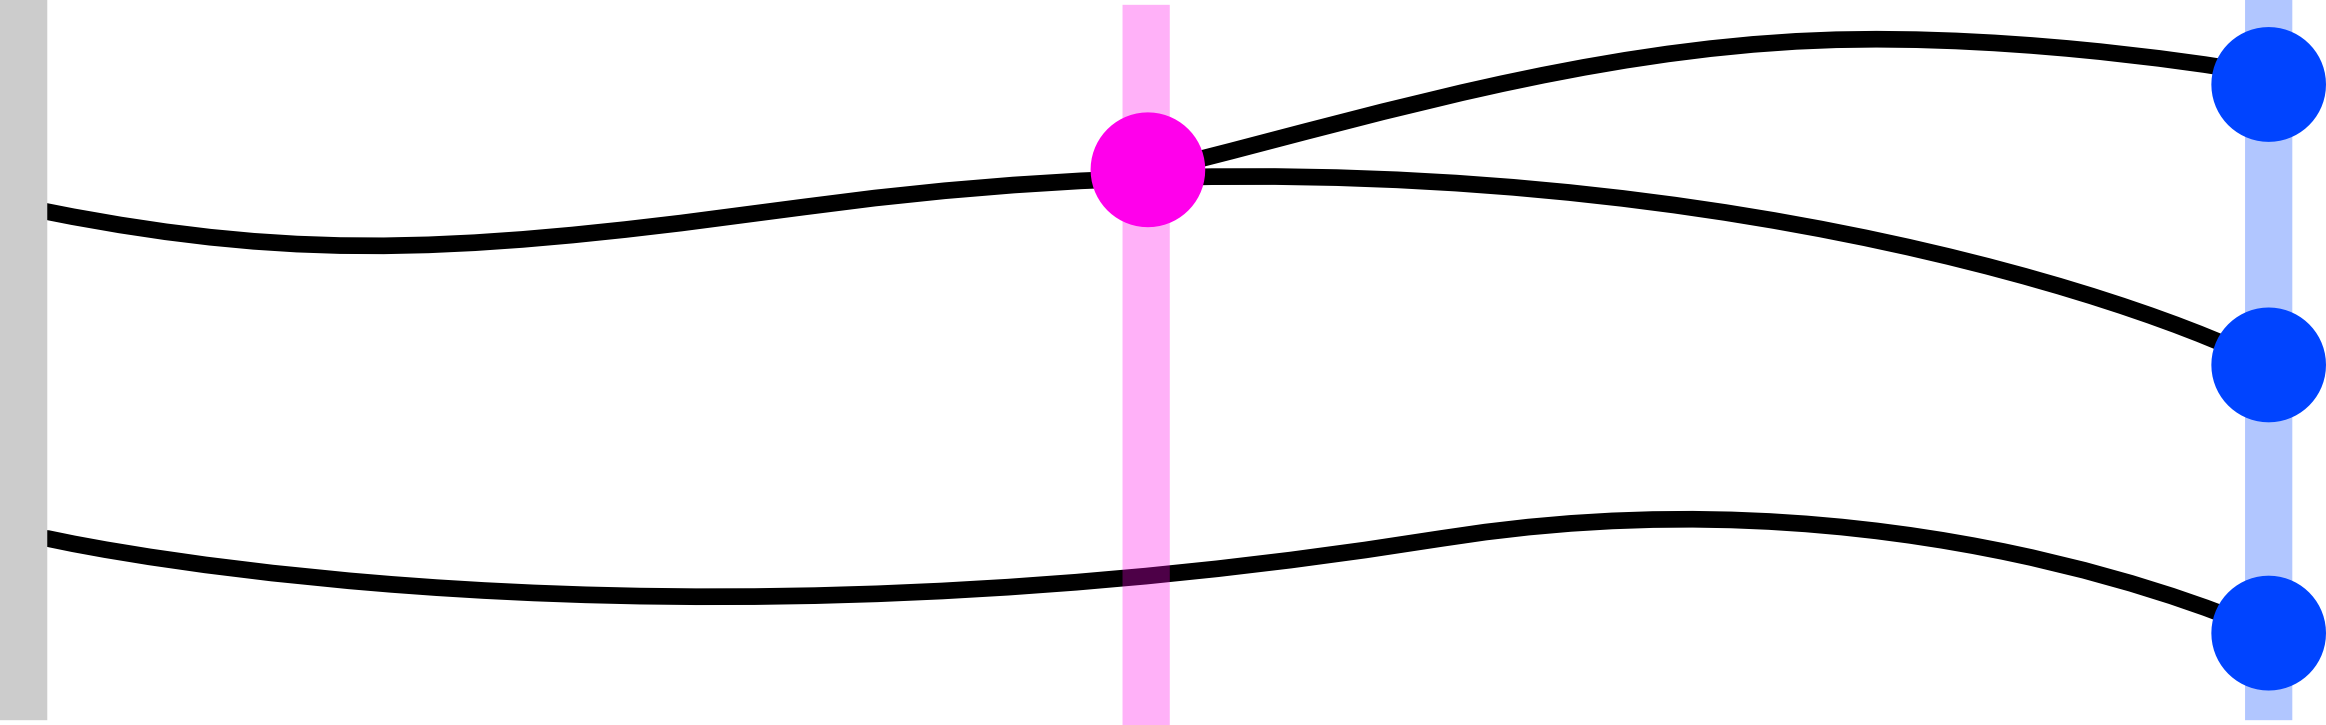
\includegraphics[width=440.25pt,height=132.05pt]{ch4/fig/distance_gen.png}};

% Text Node
\draw (4,181.46) node [anchor=north west][inner sep=0.75pt]    {\Large $s=\ 0\ =\ t-D_{t}( u,w)$};
% Text Node
\draw (285,180.46) node [anchor=north west][inner sep=0.75pt]    {\Large $s=t-D_{t}( u,v)$};
% Text Node
\draw (570,180.46) node [anchor=north west][inner sep=0.75pt]    {\Large $s=t$};
% Text Node
\draw (597,13.4) node [anchor=north west][inner sep=0.75pt]    {\Large $u$};
% Text Node
\draw (596,82.4) node [anchor=north west][inner sep=0.75pt]    {\Large $v$};
% Text Node
\draw (595,150.4) node [anchor=north west][inner sep=0.75pt]    {\Large $w$};

\end{tikzpicture}}
    \caption{Genealogical distances between individuals $u,v,w\in {\cal N}_t$. The pink particle is the most recent common ancestor of $u$ and $v$.}
    \label{fig:distance_gen}
\end{figure}

%In the case  
%$u=v$, we set $D_{KT}(u, u) = 0$. 
Denote by ${\cal N}_t$ be the set of individuals alive at time $t$ and $|{\cal N}_t|$ be the cardinal of this set.
Conditional on the event $\{{\cal N}_t\geq k\}$, let 
$(U_1, \dots, U_k)$ be $k\geq 1$ individuals
sampled uniformly \emph{without replacement} from ${\cal N}_t$.

We introduce the process
$({\cal C}^{k}_{s,t})_{s \in [0, t]}$ with values in the partitions of
$\{1,\dots, k\}$ satisfying that
\[
    \forall \tau\leq t, \ \ i \sim_{{\cal C}^{k}_{s,t}} j\ \iff\
  D_{t}(U_i, U_j)\ \leq\  s.
\]
This partition-valued process process encodes the subforest spanned by the sample $(U_i)_{i \leq k}$. Let $({\cal C}^{k,K}_{s,T})_{s \in [0,T]}$ be the process $({\cal C}^{k}_{Ks,KT})_{s\in [0,T]}/K$, where the distances are rescaled by $K$.

\medskip

We recall from~\cite{Kingman:1982aa} that the $k$-Kingman coalescent with rate $r>0$ is the partition-valued process starting from the partition of $\{1,\ldots, k\}$ in singletons and such that every pair of blocks merges at rate $r$.
\begin{thm}[Convergence of the genealogies]\label{thm:main_multitype}
     Assume that the initial rescaled population size $z_K\in \R_+^E$ satisfies that
     \[z_K\ \underset{K\to\infty}{\longrightarrow}\ \tilde h,\]
     in probability. Let $T>0$. Then, under Assumption~\ref{hyp:kingman}:
         \begin{enumerate}
    \item[(i)] The following holds in probability
        \[
            \adjustlimits\lim_{K \to \infty} \sup_{0 \leq t \leq KT}  \lVert Z_t - \tilde h\rVert \ =\ 0.
        \]
    \item[(ii)] Conditional on  the event 
    $\{\big| {\cal N}_t\big| \geq k\}$, 
    \[
        \lim_{K \to \infty} {\cal C}^{k,K}_{\cdot, T}
       \ =\ \mathcal{K}^k_{\cdot ,T},
    \]
    in distribution for the Skorohod topology, where $\mathcal{K}^k_{\cdot ,T}=(\mathcal{K}^k_{s,T})_{ s \in [0, T]}$ is a $k$-Kingman coalescent with rate $\bar m_2$. 
    \end{enumerate}
\end{thm}

\begin{rem}
Proposition \ref{Ch4:prop:kurtz} and Assumption \ref{hyp:kingman}, the event $\{|{\cal N}_t|\geq k\}$ has probability converging to $1$ as $K\to\infty$. 
We point out that the first point of Theorem~\ref{thm:main_multitype}
is an extension of Kurtz's result to the longer timescale $O(K)$.
\end{rem}

Theorem~\ref{thm:main_multitype} shows that, despite the interaction between ecological and evolutionary dynamics at the microscopic level (reproduction depends on both the underlying structure and the current state of the population), these two mechanisms decouple asymptotically. In the large population limit, the population density rapidly converges to the stable equilibrium of the limiting dynamical system. On the longer evolutionary timescale, the structure of the population affects the genealogy only through the effective coalescence rate, which determines the effective population size $N_e$. The shape of the genealogy evolves independently of the transient ecological fluctuations and is asymptotically described by the Kingman coalescent. This separation of timescales is reminiscent of the structured coalescent of~\cite{nordborg_separation_2002} in the regime of fast migration, where the distribution of types in the population equilibrates before coalescence events occur. Our setting, however, is substantially more general. Since \cite{nordborg_separation_2002} starts directly from the structured coalescent, reproduction is assumed to be both local (offspring inherit the type of their parent) and binary. By contrast, our population model allows for a broader class of reproduction mechanisms, and consequently Theorem~\ref{thm:main_multitype} recovers a much wider range of effective population sizes.

\subsection{Methodology and outline of the article}
\paragraph{Heuristics on the methodology.}
The proof of Theorem~\ref{thm:main_multitype} relies on a recursive moment formula, which is stated in Theorem~\ref{thm:many_to_few} and proved in Section~\ref{Ch4:sec:many_to_few}.
Since the recursive formula is the cornerstone of our approach, we first explain the main ideas and stress the conceptual novelty of our methodology before outlining the organization of the paper. 

Theorem~\ref{thm:many_to_few} presents a recursive formula that provides a connection between the backward description of the genealogies to a forward-in-time process called \emph{neutral fractions}. The idea is, as in~\cite{AFRS_2025}, to decompose the genealogy at its first coalescing point.
The connection between backward-in-time coalescent processes and neutral fractions is encoded in the recursive moment formula by a positive semigroup, which is introduced in Section~\ref{Ch4:sec:semigroup} and is central to our approach. In section~\ref{Ch4:sec:spine_process}, we give a Feynman--Kac representation of this semigroup, so that the semigroup rewrites as a functional of so-called spinal process in which immortal lineages are distinguished.


We expect the recursive formula to extend to a very broad class of population models, well beyond finite type spaces and Assumption~\ref{hyp:kingman}.
Indeed, the proof of Theorem~\ref{thm:many_to_few} only requires the strong Markov property and that the population can be split into subpopulations so that the neutral fractions are well-defined.
Thus, the formula is of intrinsic interest, for this reason we wrote it in the self-contained Section~\ref{Ch4:sec:methodology}.

To understand the role of the sampling function used in the proof of our main result, it is useful to first recall the linear (non-interacting) setting. For the critical multitype Galton--Watson process with mean matrix $M(\tilde h)$, the Perron--Frobenius eigenvector $h$ is a harmonic function that assigns to each type its \emph{reproductive value}: the long-term contribution of an individual of that type to future generations. Introduced by~\cite{fisher_genetical_1999}, reproductive values refine the classical notion of fitness by accounting not only for the number of offspring produced but also for their long-term reproductive success. In~\cite{Foutel_Schertzer}, sampling individuals according to their reproductive values naturally yields a martingale change of measure and greatly simplifies the analysis of genealogies.
In the interacting setting, the fixed reproductive value is replaced by a state-dependent function 
\[ 
(x,z)\ \longmapsto\ H_x(z),
\] 
 which may be interpreted as a \emph{dynamical reproductive value}. Its existence and application in the context of stochastic neutral fractions come from the recent work of~\cite{Julie_Zsofia}. This function compensates the fluctuations in the population density. 
 In particular, the first-order terms of the linearisation of the density projected onto $H$ vanish automatically. 

From there, the remaining ingredients come from stochastic analysis. If the population composition converges to the stable equilibrium of the limiting dynamical system from~\eqref{Ch4:eq:mean_dynamical_system}, then the semigroup converges to a constant limit.  
Using this estimate, the recursive formula of Theorem~\ref{thm:many_to_few} can be closed explicitly, yielding an explicit expression for the distribution of the limiting genealogy.

We emphasize that this study presents more than a straightforward adaptation of the arguments developed in~\cite{AFRS_2025} to the multitype setting. Indeed, the methodology that we used in the scalar case relies heavily on the one-dimensional structure of the model and does not readily generalize to several types, primarily because of noncommutativity issues. 
The main conceptual contribution of the present work is the introduction of the dynamic reproductive value, which in the scalar case corresponds to the inverse function $z\mapsto 1/z$ and yields a natural state-dependent sampling function.
 As a consequence, unlike in~\cite{AFRS_2025}, no exponential penalization is required to ensure the finiteness of the moments. Besides making the multitype stochastic analysis possible, this approach provides a unified and much more natural framework for studying genealogies in interacting population models. Indeed, it allows us to work directly with random coalescent variables rather than with a measure-valued recursive formula, see~\citet[Theorem~2.3]{AFRS_2025}.

\paragraph{Outline of the article.} \jj{à reprendre une fois qu'on aura mis les choses dans l'ordre final.}\ma{ok, j'ai reformulé je pense qu'on a l'ordre final-ish}
After planarizing the problem and formally introducing the topological objects in Section~\ref{Ch4:sec:objects}, we define an important nonconservative semigroup in Section~\ref{Ch4:sec:semigroup}. In particular, we give a Feyman--Kac representation of the semigroup, which becomes conservative for a new so-called spinal process introduced in Section~\ref{Ch4:sec:spine_process}.
 Then, Section~\ref{Ch4:sec:methodology} details the methodology. We state a recursive moment formula for planar gene, which relates the semigroup to the genealogies. We prove this Theorem~\ref{thm:many_to_few} in Section~\ref{Ch4:sec:many_to_few}. The remainder of the article is devoted to proving the main result by applying this recursive formula to structured density-dependent branching populations satisfying Assumption~\ref{hyp:kingman}, and thereby prove Theorem~\ref{thm:main_multitype}.
In Section~\ref{Ch4:sec:katz}, we construct the sampling function by exploiting the stability of the limiting dynamical system and derive the associated martingale change of measure.
The last three sections are dedicated to the proof of Theorem~\ref{thm:main_multitype}.
Section~\ref{Ch4:sec:heuristics} is a heuristic section that outlines the flow of the proof.  There, we state the main intermediate results and present some sketches for the proofs, which will be formalized in the last three technical sections. Building on these intermediate results, we complete the proof of Theorem~\ref{thm:main_multitype} in Section~\ref{Ch4:sec:debiaising}.
 Section~\ref{Ch4:sec:calcul_sto} contains the main stochastic analysis: In a first step, we prove convergence of the density process to an asymptotically stable equilibrium of a dynamical system and at which the reproduction mechanism is critical. Building on this result, we establish convergence of the spinal process to a stationary measure. This step constitutes the main technical challenge of the paper, and for this reason we restrict our analysis to finite type spaces rather than treating the general arbitrary setting.
Using the concentration results, in Section~\ref{Ch4:sec:convergence} we derive the limit of the semigroup. Finally in Section~\ref{Ch4:sec:fin_preuve}, we combine these ingredients with the recursive formula to close the recursion.
\section{Forests and genealogies}\label{Ch4:sec:objects}

We introduce a planarization of the problem. We will link the genealogy of the particle system presented in Section~\ref{Ch4:sec:model} to the study of random planar objects called \emph{planar coalescent processes}. Their construction is detailed in this section.

\subsection{Marked chronological planar forests}\label{Ch4:sec:Ulam_Harris}
The population model introduced in Section~\ref{Ch4:sec:model} naturally comes equipped with a genealogy. Since such a construction is rather standard (see \eg \citet{neveu_arbres_1986, otter_multiplicative_1949}), we start by providing a rather informal description of the underlying probability space. 

A {\it planar forest} $\mathbb{f}$ consists of a set of individuals indexed in the canonical Ulam--Harris--Neveu set $\mathcal{U}=\bigcup_{n\in\N}\N^n$, which induces a
planar order $\leq$. We point out that since we consider planar forests, the ancestors correspond to the first generation in the usual Ulam--Harris labeling of planar trees (see e.g.\ \cite{le_gall_random_2005}).
For any individual $u \notin \mathbb{N}$, we denote by $\anc{u}$ the unique parent of $u$.  We denote by $\succcurlyeq$ the genealogical order induced by the labeling, such that for $u,v\in\mathbb{f}$,
\[
u\succcurlyeq v\ \iff\ \begin{cases}
u=v\qquad \textit{or}\\
\exists w\in \mathcal{U},\ u=vw,
\end{cases}
\]
and by $\mathrm{Ch}(u)$ the set of 
children of $u$ in the forest $\mathbb{f}$.


A {\it  marked chronological (planar) forest} $\mathbb{F}$ is a planar forest where each individual $u$ is equipped with a birth time $\lambda_u \geq0$ and death time $\theta_u\geq0$ with the constraint that 
$\theta_u \geq \lambda_u$. We further assume that for $u\notin\N$  $\lambda_u=\theta_{\anc{u}}$ and for $u\in\N$, $\lambda_u=0$. In other words, the birth time of a particle corresponds to the death time of its parent, with the convention that the birth time of ancestral individuals is zero. Each individual is further equipped  with a mark (or {\it type})  $X^u\in E$. 

Denote by 
$\mathcal{N}_t\equiv 
\mathcal{N}_t(\mathbb{F})$ the set of particles alive at time~$t$, that is the set of individuals $u$ with $t\in[ \lambda_u,\theta_u)$. Finally, 
the \textit{density process} is defined as
\[
Z_t\ \coloneqq\ \frac{1}{K}\sum_{u\in\mathcal{N}_t} e_{X^u}.
\]
For $t\geq 0$ and $u, v\in \mathcal{N}_t$ such that $u$ and $v$ descend from the same root, 
 $ u\wedge v$ denotes the most recent common ancestor to $u$ and $v$ and
 \[
 t -\theta_{u\wedge v}
 \] 
 is their genealogical distance, with the convention that this is equal to $0$ when $u=v$. If $u$ and $v$ descend from different roots in the planar forest, we set their genealogical distance to be $\infty$.

\medskip


Let $z$ such that $z K \in \N^E$. We define $\Prob_{z}$ as the measure on marked chronological forests defined recursively such that 
\begin{enumerate}
\item The density of types at time $0$ is $z$. More precisely, the set of roots is $\mathcal{N}_0=\{1,2,\dots,K\norm{z}\}$ and the vector giving the types of the roots $(X^u)_{u\in \mathcal{N}_0}$ is drawn uniformly conditional on $\sum_{u\in \mathcal{N}_0} e_{X^u} = Kz$.
\item For all $x\in E$, individuals with type $x$ alive at time $t$ branch according to the density-dependent rate $q_{x}(Z_t)$ and 
at every birth event, the ordering of children  is chosen uniformly at random.
\end{enumerate}

Let $k \ge 1$ and let $\bm{x} \in E^k$ be a vector of types. We now define a second planarization that is distinct from the first only by imposing the types of the first $k$ individuals to $\bm{x}$. Formally,
introduce the space 
\begin{equation}\label{Ch4:eq:space_k_types}
\mathscr{D}_{k}\ \coloneqq\ \Big\{(z, \bm{x})\in \{n/K,\ n\in \N^{E}\}\times  E^k:\ \forall x\in E,\ \sum_{i=1}^k \1_{x^i=x} \leq Kz_x \Big\}
\end{equation}
that corresponds to pairs $(z, \bm x)\in \{n/K,\ n\in \N^{E}\}\times  E^k$ with ${\bm x}$ an `admissible' sample for the density $z$.  Note that $\mathscr{D}_k$ depends implicitely on $K$.
For any $(z,\bm x) \in \mathscr{D}_{k}$, we introduce $\Prob_{z,\bm x}$ as the probability measure under which:
\begin{itemize} 
    \item Types are assigned to the first $k$ individuals (labeled $\{1,\ldots, k\}$) according to ${\bm x}$. The remaining types at time $t=0$ are assigned uniformly, consistently with $K z - \sum_{i=1}^k e_{x_i}$.
    \item For all $x\in E$, individuals with type $x$ alive at time $t$ branch according to the density-dependent rate $q_{x}(Z_t)$ and 
at every birth event, the ordering of children  is chosen uniformly at random.
\end{itemize}



\subsection{Planar  coalescents}
\label{Ch4:sec:model_formal}


We now introduce the planar coalescent  associated with a planar marked chronological forest together with some useful notation.
We say that a partition of $\{1,\ldots,k\}$ is \emph{planar} if the elements of each block are consecutive -- consequently, its blocks can also be canonically ordered consecutively. These ordered partitions are sometimes called \emph{compositions of $k$}. For example, $\tilde \pi=\{\{1,2\},\{3\},\{4,5\}\}$ is a planar partition of $\{1,2,3,4,5\}$, while $\pi=\{\{1,3\},\{2,4,5\}\}$ is not. An ordered partition $\tilde \pi_1$ is \emph{nested} into $\tilde \pi_2$ if $\tilde \pi_{2}$ is obtained by merging together a \emph{successive} number of blocks in $\tilde \pi_1$. For example, $\{\{1,2\},\{3\},\{4\} ,\{5\}\}$ is nested in $\{\{1,2\},\{3\},\{4,5\}\}$. We denote by $|\tilde\pi|$ the number of blocks in the partition $\tilde \pi$. For example we have $\big|\{\{1,2\},\{3\},\{4,5\}\}\big|=3$.

Let $k\geq 0$. A function $\tilde{\pi}_\cdot = (\tilde \pi_s)_{s\geq0}$ is called a \emph{planar $k$-coalescent}  if it is a càdlàg function with values in the space of ordered partitions of $k$ such that for any $s'\geq s$, $\tilde \pi_{s}$ is nested into $\tilde \pi_{s'}$. 
We denote by $\mathbb{G}_{k}$  the set of planar $k$-coalescents; we endow it with the Skorohod topology and set
\[
\mathbb{G}\ \coloneqq\ \bigcup_{k\geq 0}\mathbb{G}_{k}.
\]
with the convention that $\mathbb{G}_0$ only contains the constant function equal to the empty partition $\emptyset$.

For $\tilde \pi_{\cdot}\in\mathbb{G}_k$, denote by
\[
\tau\big(\tilde \pi_{\cdot}\big)\ \coloneqq \ \inf \big\{ s \ge 0 : |\tilde\pi_s|< k\big\},
\]
 the first time when the value of the planar coalescent $\tilde\pi_{\cdot}$ is a partition with strictly less than $k$ blocks. We introduce the pruning function
\[ \Theta:\mathbb{G}\longmapsto \mathbb{G},\]
as the function that maps a planar coalescent $\tilde\pi_{\cdot}$ to the planar coalescent obtained by pruning $\tilde \pi_{\cdot}$ at time $\tau\big(\tilde \pi_{\cdot}\big)$. More precisely:
\begin{itemize}
  \item When $\tau\big(\tilde \pi_{\cdot}\big)<\infty$, $\Theta\big(\tilde \pi_{\cdot}\big)$ is the planar coalescent obtained by removing the trajectory up to the first coalescence event from $\tilde \pi_{\cdot}$ and re-indexing the blocks so that the pruned coalescent starts from the singleton configuration. 
  
  \item When $\tau(\tilde{\pi}_\cdot)=\infty$, we arbitrarily set $\Theta(\tilde{\pi}_\cdot)=\emptyset\in \mathbb G_0$.
\end{itemize}
  In particular, $\Theta(\tilde \pi_\cdot)\in \mathbb{G}_{j}$ for some $j<k$.
We
refer to Figure~\ref{fig:alternative_chrono_marked} for an
illustration.


\bigskip



Let us now consider a marked chronological forest $\mathbb{F}$ as introduced in Section \ref{Ch4:sec:Ulam_Harris}. Let $t>0$ and
assume that $|{\cal N}_t|\neq \emptyset$. Let 
$v_1\leq  \cdots\leq  v_{k}$ be $k$ ordered individuals in ${\cal N}_t$, allowing for repetition. 
For such a realization, 
define the partition valued process $\tilde\Pi_{\cdot,t}^{\bm{v}} = (\tilde\Pi^{\bm{v}}_{s,t})_{s \geq 0}$ as the ordered coalescent in $\mathbb{G}_k$ defined as
\begin{equation*}
\forall s\leq t, \quad
    i \sim_{\tilde\Pi^{\bm{v}}_{s,t}} j\ 
   \ \iff\ \theta_{v_i \wedge v_j}\ \geq\ t - s,
\end{equation*}
and for $s\geq t$, set $\tilde \Pi^{\bm v}_{s,t}=\tilde \Pi^{\bm v}_{t,t}$, i.e., we freeze the coalescent after time $t$. 

\begin{rem}
If $\tau(\tilde\Pi^{\bm v}_{\cdot,t})=0$, then it means that at least one particle was sampled multiple times. If at time $t$ no coalescences happened, $\tilde\pi_t$ is the partition of $\{1,\ldots,k\}$ in singletons and $\tau(\tilde\Pi^{\bm v}_{\cdot,t})=\infty$.
\end{rem}


\subsection{The planar $(H,k)$-coalescent}
Consider an arbitrary positive function
\begin{equation*}
  H: \left\{\begin{aligned}
   & E\times \R^E_+\ \longrightarrow \R^*_+\\
  &(x,z)\ \longmapsto\ H_x(z).
  \end{aligned}\right.
\end{equation*}
For any $z\in\R_+^E$ and $\bm x= (x^1,\ldots, x^k)\in E^k$, we introduce the notation
\begin{equation}\label{Ch4:eq:cal_H^k}
\mathcal{H}:
\left\{\begin{aligned}
&\R^E\times E^k\  \longrightarrow\ \R_+^*\\
&(z,\bm x)\ \longmapsto\ \prod_{i=1}^k H_{x^i}(z).
  \end{aligned}\right.
\end{equation}
We make the assumption that the population process and the function $H$ satisfy, for all initial conditions $z\in\N^E/K$ and positive time $t>0$, that 
\begin{multline}\label{Ch4:eq:normalizing_constant_manytofew}
 \kappa^{k}_{t}(z)\ \coloneqq\ \E_{z}\Big[ \sum_{\bm v:v_1, \ldots, v_k\in \mathcal{N}_t}\mathcal{H}\big(Z_t,\bm X^{\bm v}\big)\Big]\ 
=\ \E_{z}\Big[ \sum_{\bm v:v_1, \ldots, v_k\in \mathcal{N}_t}\prod_{i=1}^k H_{X^{v_i}}(Z_t)\Big]\\
 =\  K^k \E_{z}\big[ \big\langle Z_t, H(Z_t)\big\rangle^k \big]\ <\ \infty,
\end{multline}
with the convention that the RHS inside the expectation is $0$ when ${\cal N}_t=\emptyset$. 

\begin{defn}[$(H,k)-$coalescent]\label{def:Hk-coal}
Let $k\geq 1$.
We define a random variable $(\tilde \Pi^k_{\cdot,t}, Z^k_t, \bm X^k_t)$  with values in $\mathbb{G}_{k}\times \mathscr{D}_{k}$ such that any measurable bounded function $\varphi: \mathbb{G}_{k}\times \mathscr{D}_{k} \to \mathbb{R}$
\begin{equation*}
  \E_{z}\Big[\varphi\big(\tilde{\Pi}^k_{\cdot,t}, Z^k_t, \bm X^k_t\big)\Big]\ =\ 
    \frac{1}{\kappa^k_{t}(z)}  \E_{z}\bigg[
\sum_{\bm v:v_1 , \ldots ,v_k\in\mathcal{N}_t }\varphi(\tilde\Pi^{\tilde{\bm v}}_{\cdot,t} , Z_t, \bm X^{\bm v})\mathcal{H}\big(Z_t,\bm X^{\bm v}\big)\bigg].
\end{equation*}
\end{defn}


In particular, we have
\begin{equation}\label{Ch4:eq:distinct_particles}
  \E_{z}\Big[ \1\big(\tau(\tilde{\Pi}^k_{\cdot,t})>0\big) \varphi\big(\tilde{\Pi}^k_{\cdot,t}, Z^k_t, \bm X^k_t\big)\Big] =
    \frac{k!}{\kappa^k_{t}(z)}  \E_{z}\bigg[ \sum_{\bm v:v_1 <  \ldots < v_k\in\mathcal{N}_t }\varphi(\tilde\Pi^{{\bm v}}_{\cdot,t} , Z_t, \bm X^{\bm v}) \mathcal{H}\big(Z_t,\bm X^{\bm v}_t\big)\bigg],
\end{equation}
where we used the fact that if there exists some repetition in ${\bm v}$, then
\[
\tau(\tilde{\Pi}_{\cdot,t}^{\bm v})\ =\ 0.
\]



\begin{rem}
The construction above amounts to first considering a random variable $Z^k_t$, which distribution corresponds to that of the initial density process at time $t$, biased by the quantity $\langle Z_t, H(Z_t)\rangle^k$, which is well defined because of our condition~\eqref{Ch4:eq:normalizing_constant_manytofew}. That is, for all $f$ bounded measurable and $z\in \N^E/K$,
\[
\E_z\big[f(Z^k_t)\big]\ =\ \frac{1}{\kappa^{k}_{t}(z)}\E_z\Big[f(Z_t)\big\langle Z_t, H(Z_t)\big\rangle^k\Big].
\]
Then, conditional on $\mathcal{F}_t$, let $\bm U=(U_1, \ldots, U_k)$ be a $k$-tuple of individuals, each independently sampled with replacement from the population at time $t$ with probability
\[
\forall u\in \mathcal{N}_t,\ 1\leq i\leq k,\quad \Prob \big( U_i=u \,\big|\, \mathcal{F}_t\big)\ =\ \frac{H_{X^{\jjn{u}}}(Z^k_t)}{\langle Z^k_t, H(Z^k_t)\rangle}.
\]
We order the sampled individuals according to the planar order $\leq$, denote by $\tilde{\bm U}$ the resulting ordered sample and by $\bm X^{\tilde{\bm U}}$ the types of the sampled individuals once sorted (allowing once again for repetitions).
Then, the law of $(\tilde \Pi^k_{\cdot,t}, Z^k_t, \bm X^k_t)$ is that of $(\tilde\Pi^{\tilde{\bm U}}_{\cdot,t}, Z^k_t, \bm X^{\tilde{\bm U}})$.
\end{rem}


\begin{rem}
Let us close this section with an important remark. 
Let $\tilde h$ and $h$ be as in Assumption~\ref{hyp:kingman}. Then \es{to be completed: I will do it} 
\end{rem}


\es{not sure this is true} \jj{Oui c'est pas la planar version du Théorème (pas le bon $H$ mais aussi il y a vite fait le conditionnement qui entre en jeu): juste dire que tilde = planar et laisser tomber pour l'instant le lien avec le thm ? Ou alors dire plus flouement que la compréhension de cette planar version, avec un H bien choisi, permettra de prouver le Thm, sans préciser plus.}\ma{ok pour la version plus floue (TODO je m'en occuperai)}
The \emph{tilde} notation emphasizes that this is the ordered (planar) version of the genealogy studied in Theorem~\ref{thm:main_multitype}.
 To obtain the usual partition-valued genealogy, we apply the permutation induced by the sampling order of the individuals. That is, if $\sigma$ denotes the permutation mapping the planar ordering of the sample to the chosen labeling and choosing $H\equiv 1$, we recover a (unordered) partition-valued process by permuting the labels of the leaves of $\big(\tilde\Pi_{s,t}^k)_{s\geq 0}$ according to $\sigma$. Calling  $(\Pi_{\cdot,t}^k) :=\sigma(\tilde\Pi_{\cdot,t}^k)$ this object, its definition coincides with the coalescent introduced in the introduction (see Section~\ref{Ch4:sec:results}).


\begin{figure}[h!]
    \centering
\resizebox{0.95\textwidth}{!}{
\begin{tikzpicture}[x=0.75pt,y=0.75pt,yscale=-1,xscale=1]
%uncomment if require: \path (0,468); %set diagram left start at 0, and has height of 468

%Image [id:dp5445641053080238] 
\draw (385,248.53) node  {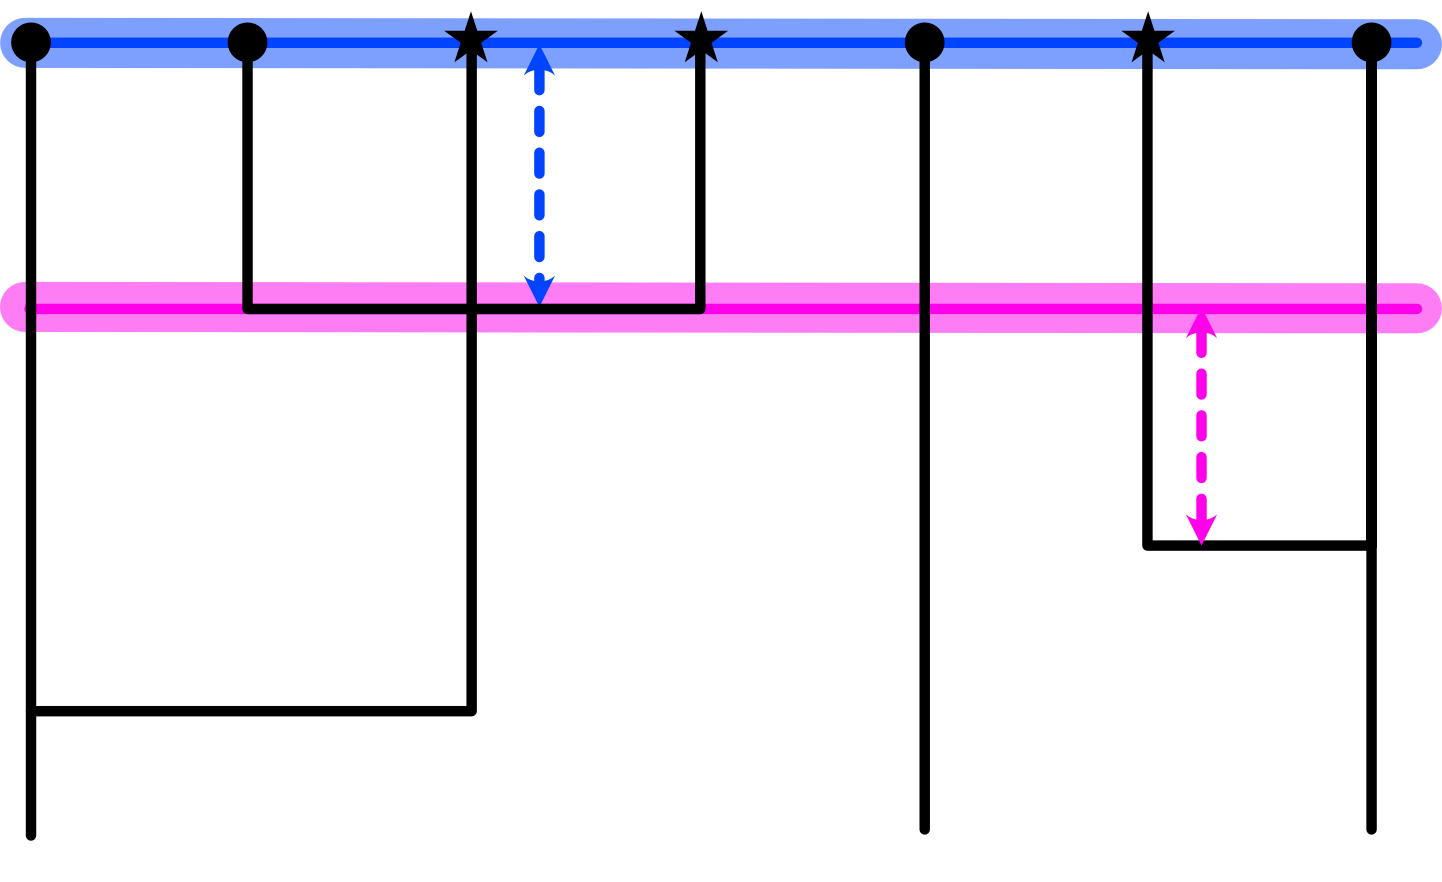
\includegraphics[width=550.5pt,height=366.8pt]{ch4/fig/planar_coal_multitype.png}};

% Text Node
\draw (760,165) node [anchor=north west][inner sep=0.75pt]  [font=\Large,opacity=1 ]  {$t=T-\tau(\tilde{\pi }_{\cdot })$};
% Text Node
\draw (760,20) node [anchor=north west][inner sep=0.75pt]  [font=\Large,opacity=1 ]  {$t=T$};
% Text Node
\draw (760,460) node [anchor=north west][inner sep=0.75pt]  [font=\Large ,opacity=1 ]  {${\displaystyle t=0}$};
% Text Node
\draw (304,77.4) node [anchor=north west][inner sep=0.75pt]  [font=\LARGE,color={rgb, 255:red, 31; green, 119; blue, 180 }  ,opacity=1 ]  {$\textcolor[rgb]{0.15,0.2,1}{\tau(\tilde{\pi }_{\cdot })}$};
% Text Node
\draw (641,222.4) node [anchor=north west][inner sep=0.75pt]  [font=\LARGE,color={rgb, 255:red, 31; green, 119; blue, 180 }  ,opacity=1 ]  {$\textcolor[rgb]{1,0.05,0.98}{\tau(\tilde{\pi } '_{\cdot})}$};
% Text Node
\draw (742,165) node [anchor=north west][inner sep=0.75pt]  [font=\huge,color={rgb, 255:red, 246; green, 21; blue, 255 }  ,opacity=1 ,rotate=-359.98]  {$\begin{drcases}
 \\\\
 \\\\
 \\\\
 \\
\end{drcases}$};
% Text Node
\draw (865,20) node [anchor=north west][inner sep=0.75pt]  [font=\Large,color={rgb, 255:red, 43; green, 45; blue, 255 },opacity=1 ]  {$\begin{drcases}
 \\\\
 \\\\
 \\\\
 \\\\
 \\\\
 \\\\
 \\
\end{drcases}$};
% Text Node
\draw (790,220) node [anchor=north west][inner sep=0.75pt]  [font=\LARGE,color={rgb, 255:red, 31; green, 119; blue, 180 }  ,opacity=1 ,rotate=-90.52]  {$\textcolor[rgb]{1,0.05,0.91}{\tilde{\pi } '_{\cdot } =\Theta(\tilde{\pi }_{\cdot }) \in \mathbb{G}_{5}}$};
% Text Node
\draw (915,220) node [anchor=north west][inner sep=0.75pt]  [font=\LARGE,color={rgb, 255:red, 31; green, 119; blue, 180 }  ,opacity=1 ,rotate=-90.52]  {$\textcolor[rgb]{0.04,0.22,1}{\tilde{\pi }_{\cdot} \in \mathbb{G}_{7}}$};


\end{tikzpicture}
   }
    \caption{Example of a planar marked coalescent on the space type $E=\{\bullet,\star\}$. In blue: a planar marked coalescent $(\tilde\pi_\cdot, \bm x)\in \mathbb{G}_{7}\times E^7$, where $\bm x=(\bullet,\bullet,\star,\star,\bullet,\star, \bullet)$. The first coalescent event is given here by $\tilde{\pi}_1=\tilde\pi_{2,3}$, and the planar coalescent $(\tilde \pi '_s)_{s\geq 0} =\Theta\big((\tilde \pi_s)_{s\geq 0}\big)\in \mathbb{G}_{5}$ obtained from pruning at the first coalescing point is pictured in pink.}\label{fig:alternative_chrono_marked}
\end{figure}




\section{The $(H,k)$-semigroup} \label{Ch4:sec:semigroup}
In this section, we introduce a semigroup associated with the function $H$, tracking the progeny of $k$ focal individuals after size biasing of the population by $\mathcal{H}$. 
This is a semigroup that will play 
a crucial role in our description of the statistics of the $H$-coalescents (see Theorem \ref{thm:many_to_few} below).

One important property of this semigroup is that it is usually non-conservative. However, in Section \ref{sect:FK}, we will derive a Feynman-Kac representation of the semigroup in terms of a Markov process that can be thought of as the joint law of $k$ distinguished lineages within the population. 





\begin{defn}[$(H,k)$-semigroup]\label{def:def_P_semigroup} Let
 $k\in\N$. The (non-conservative) semigroup $(\mathcal{M}^k_t)_{t\geq 0}$ is defined as \begin{equation}\label{Ch4:eq:def_P_semigroup}
\forall (z,{\bm x})\in\mathscr{D}_{k}, \ \ \mathcal{M}^k_t\psi( z, \bm x)\ \coloneqq\ \frac{1}{\mathcal H(z,\bm x)}\E_{z,\bm x}\Big[\sum_{ \substack{\bm u: u_1, \ldots, u_k \in \mathcal{N}_t\\ \forall i, u_i\succcurlyeq i}}\psi\big(Z_t, \bm  X^{\bm u}\big)\mathcal{H}\big(Z_t,\bm X^{\bm u}\big) \Big],
\end{equation}
where $\psi \colon \mathscr{D}_k \to \R$ 
is any bounded measurable function. (Note that  the RHS is always finite by (\ref{Ch4:eq:normalizing_constant_manytofew}).) 
\end{defn}


 \begin{rem}
\es{explain more. this is not really accurate.} \ma{je trouve ça intéressant de garder le lien (pour faire un parallèle avec~\cite{Julie_Zsofia} notamment)} \jj{dans ce cas, on rajoute la citation ?}\ma{oui}
Let us draw a parallele betwwe with the $(H,k)$-semigroup and the approach developped in~\cite{Julie_Zsofia}, who used the description of neutral fractions to derive convergence of a regulated SDE model to the Wright--Fisher diffusion.
Looking at the definition of $(\mathcal{M}^k_t)_{t\geq 0}$, at time $t$, the condition $u_i\succcurlyeq i$ in the definition of $\mathcal{M}^k_t$ restricts $u_i$ to be a descendant of the $i^{th}$ distinguished particle. Thus, the sum in~\eqref{Ch4:eq:def_P_semigroup} ranges over $k$-tuples of descendants, with one descendant chosen from each of the $k$ distinguished lineages. 
If we think of assigning $k$ distinct alleles at time $0$ to the $k$ distinguished particles, then the descendants of that particle at time $t$ form the subpopulation carrying allele $i$. The factor $\sum_{u_i\succcurlyeq i}H_{X^{u_i}}(Z_t)$ can be interpreted as the weight of the neutral fraction associated with the $i^{th}$ allele, conditional on the environmental state $Z_t$. For $k=1$, $\mathcal M_t^1$ describes the evolution of the neutral fraction carried by a single initially distinguished allele. 
\jj{Toujours pas d'accord avec les deux phrases suivantes ("joint weight" -> ben il manque les sommes; "records the joint evolution" -> pas précis, dans quel sens?), reformule ou coupe carrément:}\ma{ok} For the $k>1$ allele construction, the sum runs over individuals $u_1,\ldots, u_k$ such that for all $i$, $u_i$ belongs to the $i^{th}$ neutral fraction $Z^{(i)}_t \coloneqq \sum_{u_i \in \mathcal{N}_t, u_i\succcurlyeq i}X^{u_i}$. 
The factor
$\sum_{\bm u}\mathcal H(Z_t, \bm X^{\bm u})=\prod_{i=1}^k \langle Z^{(i)}_t, H(Z_t)\rangle$ is the joint weight of the $k$ selected alleles.
%  Thus, the $k$-particle semigroup $(\mathcal{M}^k_t)_{t\geq 0}$ records the joint evolution of $k$ such neutral fractions.
 \end{rem}

\begin{rem}[Analogy with Branching processes]
To give more insight about this semigroup, observe that the model considered here encompasses the standard multitype continuous time branching process~\cite{athreya_branching_1972}  as a particular case, which is obtained by assuming that the branching rates $q_{x}$ are independent of the population density $z$. 
Let $A$ be the rate matrix of the branching process  \citep{athreya_branching_1972}. Under standard technical assumptions (irreducibility, aperiodicity), the Perron--Frobenius theorem applies, and $A$ admits a dominant eigenvalue $\rho$ and a corresponding positive right eigenvector $(h_{x})_{x\in E}$. We identify the sampling function $(x,z)\mapsto H_{x}(z)$ with the constant (in $z$) function $x\mapsto h_{x}$, so that 
$H_{x}$ is constant in $z$.
 The function $h_x$ is  harmonic and is called the reproductive value. Let us treat the case $k=1$, starting from a particle with type $x\in E$, so that $z=e_x/K$. Projecting onto the reproductive value, the process $W_t$ defined by
\[
W_t \ \coloneqq\ \e^{-\rho t} \frac{\langle Z_t,H\rangle}{H_{x}}
\]
is a nonnegative martingale.
The semigroup $\mathcal{M}^1_t$ introduced above re-writes as 
\[
\mathcal{M}^1_t\psi(z,x)\ =\  \E_{z,x}\Big[W_t \sum_{u\in \mathcal{N}_t}\psi(Z_t, X^u)\e^{\rho t}\frac{ H_{X^u}}{\langle Z_t, H\rangle }\Big]
, \]
and  we recover the so-called many-to-one formula of~\cite{kurtz_conceptual_1997} that is, the above display re-writes
\[ 
\mathcal{M}^1_t\psi(z,\bm x)\ =\  \E\big[\psi(\hat Z_t,\hat S_t)\big]
\]
where the pair of random variables $(\hat{Z}_t,  \hat S_t)$ is such that one immortal lineage called spine reproduces according to a size-biased distribution and immigrates particles into the population, while the other individuals reproduce according to the initial dynamic. The type process $\hat S_t$ along the spine of the Kesten tree evolves according to the $H$-transformed kernel described \eg in~\cite{lyons_pemantle_peres_1995}.
For $k>1$, we denote by $Z_t^{(i)}$ the rescaled count of types in the descendants at time $t>0$ of the ancestral particle labeled $i$. By the branching property, $Z_t^{(i)}$ is a multitype continuous branching process with mean matrix $M(t)$, starting from $e_{x^i}$ and we can apply the case $k=1$ to each of the subfamilies. 

In the density-dependent model, we will see that choosing it carefully, $H$ can be thought of as a ``dynamical'' reproductive value and that the $(H,k)$-semigroup rewrites in terms of a spinal process.
%  Taking $\psi\equiv \bm{1}$, the semigroup $\mathcal{M}^1_t \bm{1}$ re-writes as
% \[
% \mathcal{M}^1_t \bm{1}(z, x)\ =\ \E\Big[\frac{\langle  Z_t, H(Z_t)\rangle}{H_{x}(z)}\Big].
% \]
\end{rem}

Denote by ${\cal G}^k$  the generator of the $(H,k)$-semigroup.
By definition, for every function $\psi:\R_+^E\times E^k\to\R$ that is in the domain of $\mathcal G^k$\ffr{needs to be in the domain...}, and every $(\bm z, x)$ in the set $\mathscr{D}_{k}$ from~\eqref{Ch4:eq:space_k_types},
\[
\lim_{t\to 0}\ \frac{1}{t}\Big[\mathcal{ M}^k_t\psi(z,\bm x)-\psi(z,\bm x)\Big]\ =\ \mathcal{G}^k \psi(z,\bm x).
\]
The expression of $\mathcal{G}^k\psi(z,\bm x)$ can be directly calculated from the transition rates of the interacting particle model $(Z^k_t)_t$ introduced in Section~\ref{Ch4:sec:model_formal}.
% From the definition of the rates of the particle model introduced in Section~\ref{Ch4:sec:model_formal},
%  the jump times of the particle system from Section~\ref{Ch4:sec:model_formal} are given as a state dependent point process. When the population denstity is $z$, the instantaneous jump rate $z\mapsto z+ (n-e_x)/K$ coming from every particle with type $x$ is given by $q_x(z)\Prob(L_x(z)=n)$ for every $x\in E$ and $n\in\N^E$. From there, either the next jump comes from a particle descending from one of the ancestral labeled particle. That is, as $t\to 0$, one of the ancestral particle jumps and changes both coordinates of $\psi$ and $\mathcal{H}$.
% Or, the jump comes from a particle in the rest of the population, and the jump only affects the first coordinates. \ffr{Tout ce paragraphe n'est pas très clair je trouve. Est-ce que tu ne peux pas tout simplement dire que $\mathcal{M}^K_t$ se calcule directement à partir des taux de transitions du processus (tu peux en fait voir $\mathcal{M}^k_t\psi$ comme le semigroupe du processus $Z_t$ appliqué à une fonctionnelle bien choisie, pour laquelle l'expression du générateur est immédiate.} \jj{oui ce serait mieux (sans t'occuper encore du domaine par contre).}

% From this observation, we compute:
% \begin{align}\nonumber
% &\mathcal{G}^k\psi(z,\bm x)\  =\ \lim_{t\to 0}\ \frac{1}{t}\big(\mathcal{ M}^k_t\psi(z,\bm x)-\psi(z,\bm x)\big)\\ \label{Ch4:eq:semigroup_generator_1}
%  &\begin{multlined}[t]
%   =\  \sum_{i=1}^k  q_{x^i}(z)\\
%   \times\E\bigg[ \sum_{y\in E} \frac{L_{x^i y}(z) H_y\big(z+ \tfrac{L_{x^i}(z)-e_{x^i}}{K}\big)}{H_{x^i}(z+ \tfrac{L_{x^i}(z)-e_{x^i}}{K})}\frac{\mathcal{H}\big(z+ \tfrac{L_{x^i}(z)-e_{x^i}}{K}, \bm x\big)}{\mathcal{H}(, \bm x)} \psi\big(z + \tfrac{L_{x^i}(z)-e_{x^i}}{K}, (\bm{x}_{1:i-1}, y, \bm{x}_{i+1:k}) \big)\\ - \psi(z, \bm{x}) \bigg] \\
% +\sum_{y\in\E} \Big(Kz_y-\sum_{i=1}^k\1_{x^i=y}\Big) q_{y}(z)\E\bigg[\frac{\mathcal{H}\big(z+ \tfrac{L_y(z)-e_{x^i}}{K}, \bm x\big)}{\mathcal{H}(z, \bm x)}\psi(z + \tfrac{L_y(z)-e_{x^i}}{K},\bm x) - \psi(z, \bm{x}) \bigg].
% \end{multlined}
% \end{align}

% where we recall the notation $(\bm{x}_{1:i-1}, y, \bm{x}_{i+1:k})$ from~\eqref{Ch4:eq:insertion}.

\subsection{The $(H,k)$-spine process}\label{Ch4:sec:spine_process}
We begin by introducing in Definition~\ref{def:spine_one_particle_per_family} a Markov process representing a population in which $k$ ``spinal'' immortal lineages are distinguished.
Let $z\in\R_+^E$ and $\bm x\in E^k$. We recall from~\eqref{Ch4:eq:cal_H^k} the notation
\[
\mathcal{H}(z,\bm x)\ =\ \prod_{i=1}^k H_{x^i}(z).
\]
In addition, for all $y\in E$, we denote by  $L_y(z,\bm x)$ the random variable with values in $\N^E$ which distribution satisfies for all $f:\N^E\to \R_+$ that
\begin{equation}\label{Ch4:eq:normal_reproduction_Pk}
  \E\Big[f\big(L_{y}(z,\bm x)\big)\Big]\ =\ \frac{1}{m_y(z,\bm x)}    
\E\Big[f\big(L_{y}(z)\big)\frac{\mathcal{H}\big(z+\frac{L_{y}(z)-e_{y}}{K},\bm x\big)}{\mathcal{H}(z,\bm x)}\Big],
\end{equation}
where $m_y(z, \bm x)$ is the normalizing constant to recover a probablity distribution on $\N^E$. 

\medskip

Besides, we define the pair of r.v. $(L_{y}^{\star}(x,{\bm z}), Y_{y}^{\star}(x,{\bm z}))\in \N^E\times \E$ in the following way:
\begin{enumerate}
\item The distribution of $L^\star_y(z,\bm x)$ is characterized by the following size-biasing of $L_y(z,\bm x)$:
\begin{equation}\label{Ch4:eq:spinal_reproduction}
 \E\Big[f\big(L^\star_y(z,\bm x)\big)\Big]\ =\ \frac{1}{m^\star_y(z,\bm x)}\E\Big[f\big(L_{y}(z,\bm x)\big)\frac{\langle L_{y}(z,\bm x), H\big(z+\frac{L_{y}(z,\bm x)-e_{y}}{K}\big)\rangle}{H_y\big(z+\frac{L_{y}(z,\bm x)-e_{y}}{K}\big)}\Big],
   \end{equation}
   where $m^\star_y(z,\bm x)$ is a normalizing constant.
\item Conditional on $L^\star_{y}(z, \bm{x})=n$, the random variable $Y^\star_{y}(z, \bm{x})$ is distributed as
   \begin{equation}\label{Ch4:eq:new_spine_type}
    \Prob\big( Y^\star_y(z,\bm x) = y' \mid L^\star_{y}(z, \bm{x}) = n\big)
   \ =\
    \frac{n_{y'} H_{y'}\big(z+\frac{n-e_{y}}{K}\big)}{\big\langle n, H\big(z+\frac{n-e_y}{K}\big)\big\rangle}.
   \end{equation}
\end{enumerate}
We also introduce the biased rates
\begin{equation}\label{Ch4:eq:modified_rates_spines}
\begin{aligned}
    q_y(z, \bm{x})\ &\coloneqq\  
    q_y(z) m_y(z,\bm x)\\ 
    q^\star_y(z, \bm{x})\ &\coloneqq\  
   q_y(z) m^\star_y(z,\bm x) .
\end{aligned}
\end{equation}

\begin{defn}[$(H,k)$-spine process]\label{def:spine_one_particle_per_family}
Let $k\in\N$.
We introduce a continuous time Markov population model with $k$ distinguished particles called \emph{spines}. We describe the system by its global density $(\mathcal{Z}^k_t)$ and the types of each spinal particle denoted by $\bm{S}_t^k = (S_t^1, \ldots, S_t^k)$.  We call spinal process the process $(\mathcal{Z}^k_t, \bm S^k_t)_{t\geq 0}$, taking values in $\mathscr{D}_k$ from~\eqref{Ch4:eq:space_k_types}, whose transitions are given below. We stress that it implicitely depends on $H$.
 
 Let $(z,\bm x) \in \mathscr{D}_{k}$ be the current state of the population and let $y\in E$. 
\begin{itemize}
    \item Each of the $Kz_y-\sum_{i=1}^k \1_{x^i=y}$  non-spinal particles with type $y$ reproduces at rate $q_{y}(z,\bm x)$. Upon a reproduction event, they die and are replaced by a copy of the random variable $L_y(z,\bm x)$ defined in~\eqref{Ch4:eq:normal_reproduction_Pk}.
    \item Let $i\in\{1,\ldots, k\}$. The $i^{th}$ spinal particle reproduces at rate $q^\star_{x^i}(z,\bm x)$. Upon this reproduction event, the type of the $i^{th}$ spine transitions in $E$ from $x^i$ to the type of  one of its children. The progeny (including the new spine) and the new type of spine are given by a sample of the pair of random variables 
    \[
    \big(L^\star_{x^i}(z,\bm x),\ Y^\star_{x^i}(z,\bm x)\big),
    \]
     introduced in~\eqref{Ch4:eq:spinal_reproduction} and~\eqref{Ch4:eq:new_spine_type}.
\end{itemize}
\end{defn}

   We point out that if we set $k=1$ in~\eqref{Ch4:eq:spinal_reproduction} and~\eqref{Ch4:eq:normal_reproduction_Pk}, we recover the transitions given in the $H$-spine process of~\citet[Section 3]{Bansaye}.
Furthermore, we observe that if $k=0$, the transitions of the density processes $\mathcal{Z}^0_t$ from Definition~\ref{def:spine_one_particle_per_family} and $Z_t$ from Section~\ref{Ch4:sec:model_formal} coincide. Thus, by convention we will say that the initial process corresponds to taking $k=0$ in Definition~\ref{def:spine_one_particle_per_family}, allowing us to state results ``for all $k\geq 0$''. \jj{On fait vraiment ça dire des trucs pour $k\geq 0$ ?}\ma{oui dans la partie calcul sto}
\begin{rem}[Analogy with Branching processes]
Once again, we can recover the usual non-interacting spinal process presented in~\cite{kurtz_conceptual_1997} for (finite) multitype Galton--Watson processes from Definition~\ref{def:spine_one_particle_per_family}, when $k=1$. Indeed, assume that for all $x$, the offspring distribution $L_x$ does not depend on the population size. We set $z\mapsto H(z)\equiv  h$ to be the principal right eigenvector of the mean matrix (constant in $z$). We have that for all $y\in E$ and $\bm x\in E^k$, the bias factor in~\eqref{Ch4:eq:normal_reproduction_Pk} equals $1$, so in the Definition~\ref{def:spine_one_particle_per_family} the non spinal particles reproduce according to the initial offspring distribution, as in the usual construction from~\cite{kurtz_conceptual_1997}.  Moreover, in the spinal construction, if the current spinal particle has type $y$, its offspring distribution is changed from $L_y$ to the size-biased law 
\[
\E\Big[f\big(L^\star_y\big)\Big]\ =\ \E\Big[f\big(L_y\big)\frac{\langle L_y,h\rangle}{\rho h_y}\Big],
\]
for $\rho>0$ the principal eigenvalue. The new spine is selected at random among the progeny, with children being picked with probabilities proportional to $h_x$ when their type is $x$. This corresponds to the pair $(L^\star_y, Y^\star_x)$ in Definition~\ref{def:spine_one_particle_per_family} for $H=h$, using that $\E\big[\langle L_y, h\rangle\big]=\rho h_y$. Thus, the $(h,1)$-spine process coincides with that of~\cite{kurtz_conceptual_1997}. By the branching property, the subfamilies descending from each spine do not interact with each other. Thus, the $(h,k)$-spine process with $k>1$ corresponds to $k$ independent $(h,1)$-spine constructions  stacked together.
\end{rem}

\subsection{Feynman--Kac representation of the $(H,k)$-semigroup}
\label{sect:FK}
The main goal of this section is to derive a Feynman--Kac representation of the $(H,k)$-semigroup   $\mathcal{M}^k_t$ introduced in Definition~\ref{def:def_P_semigroup}. It is stated in the following Proposition~\ref{Ch4:prop:P_semigroup_feyman_kac}. 

We recall that ${\cal G}^k$
denotes the generator of the $(H,k)$-semigroup.
Considering the Doob $\bm{1}$-transform of $\mathcal{G}^k$ yields another generator denoted by $\mathcal{A}^k$, which is given through the usual formula:
 \begin{equation}\label{Ch4:eq:palmoswski_changegen}
 \mathcal{A}^kf\ \coloneqq\ \mathcal{G}^kf-f\mathcal{G}^k\bm{1}.
 \end{equation}
By a quick generator computation, we derive that $\mathcal{A}^k$ is the generator of the $(H,k)$-spine Markov process from Definition~\ref{def:spine_one_particle_per_family}.
\begin{prop}[Feynman--Kac representation]\label{Ch4:prop:P_semigroup_feyman_kac}
Let $k, t\geq 0$, $\psi:\R_+^E\times E^k\to \R$ a bounded and measurable functional. Then, 
\begin{equation} \label{Ch4:eq:FeynmanKac}
\forall (z, \bm x)\in {\cal D}_{k,K}, \ \ \
\mathcal{M}^k_t{\psi}(z, \bm x) \ =\ \E_{z, \bm x}\bigg[ \psi(\mathcal{Z}^k_t, \bm S^k_t) \exp\Big(\int_0^t\mathcal{G}^k\bm{1}(\mathcal{Z}^k_s,\bm S^k_s)ds\Big)\bigg],
\end{equation}
where $(\mathcal{Z}^k_t,\bm S^k_t)$ is the $(H,k)$-spine process from Definition~\ref{def:spine_one_particle_per_family}. \ffr{On a pas un problème avec l'explosion ici ? C'est le même problème de martingale locale qu'on avait dans le simple type il me semble.}
\end{prop}
\begin{proof}
Let $\widetilde{\mathcal{M}}^k_t$ be the operator defined as
\[
    \widetilde{\mathcal{M}}^k_t\psi(z, \bm{x})
    \ \coloneqq\ \E_{z,\bm x}\bigg[\psi\big(\mathcal{Z}^k_t,\bm{S}^k_t\big)\exp\Big(\int_0^t \mathcal{G}^k\bm{1}(\mathcal{Z}^k_s,\bm S^k_s)ds\Big)\bigg]
\]
for $z\in\R_+^E$, $\bm{x} \in  E^k$ and $\psi:\mathscr{D}_{k} \to \R_+$ is bounded. It is not hard to see that $(\widetilde{\mathcal{M}}^k_t)_{t \ge 0}$ is an operator semigroup on the space of bounded maps $\psi \colon \mathscr{D}_{k} \to \R$ and we will prove that $(\mathcal{M}^k_t)_{t \ge 0} = (\widetilde{\mathcal{M}}^k_t)_{t \ge 0}$ by showing that their generators coincide. 

Suppose that $\psi$ has a finite support. Then we can directly compute that, if $\widetilde{\mathcal{G}}^k$ denotes the generator of $(\widetilde{\mathcal{M}}^k_t)_{t \ge 0}$, $\psi$ belongs to the domain of $\widetilde{\mathcal{G}}^k$ and 
\[
    \widetilde{\mathcal{G}}^k\psi(z, \bm{x}) = \mathcal{A}^k\psi(z, \bm{x}) + \psi(z, \bm{x})\mathcal{G}^k\bm{1}(z, \bm{x}),
\]
where $\mathcal{A}^k$ is the generator of $(\mathcal{Z}^k_t, \bm{S}^k_t)_{t \ge 0}$. Therefore, using \eqref{Ch4:eq:palmoswski_changegen} we compute for all $\psi$ bounded,
\begin{multline*}
\frac{1}{t}\Big(\tilde{\mathcal{M}}^k_t\psi(z,\bm x)-\psi(z,\bm x)\Big)\ =\ \frac{1}{t}\Big(\E_{z,\bm x}\Big[\psi\big(\mathcal{Z}^k_t,\bm{S}^k_t\big)\Big]-\psi(z,\bm x)\Big)\\
+ \frac{1}{t}\E_{z,\bm x}\bigg[\psi\big(\mathcal{Z}^k_t,\bm{S}^k_t\big)\Big(\exp\Big(\int_0^t \mathcal{G}^k\bm{1}(\mathcal{Z}^k_s, \bm S^k_s)ds\Big)-1\Big)\bigg]. 
\end{multline*}
Since $\mathcal{A}^k$ is infinitesimal generator the spinal process $(\mathcal{Z}^k_t,\bm S^k_t)$,  
\[
\lim_{t\to 0}\ \frac{1}{t}\Big(\E_{z,\bm x}\Big[\psi\big(\mathcal{Z}^k_t,\bm{S}^k_t\big)\Big]-\psi(z,\bm x)\Big)\ =\ \mathcal{A}^k_t\psi(z,\bm x).
\]
Whereas for the second part, 
\begin{multline*}
\lim_{t\to 0}\ \frac{1}{t}\E_{z,\bm x}\bigg[\psi\big(\mathcal{Z}^k_t,\bm{S}^k_t\big)\Big(\exp\Big(\int_0^t \mathcal{G}^k\bm{1}(\mathcal{Z}^k_s, \bm S^k_s)ds\Big)-1\Big)\bigg]\\
 =\ \psi\big(z,\bm x\big)\lim_{t\to 0}\frac{1}{t}\E_{z,\bm x}\bigg[\exp\Big(\int_0^t \mathcal{G}^k\bm{1}(\mathcal{Z}^k_s, \bm S^k_s)ds\Big)-1\bigg]\\
  =\ \psi\big(z,\bm x\big)\mathcal{G}^k\bm{1}(z, \bm x),
\end{multline*}
which conludes the proof.
\jj{Attention aux domaines de générateurs... En fait je réalise que pour les caractérisation de semigroupes par leurs générateurs, je ne connais que des réfs qui parlent de semigroupes Feller (par exemple dans la bible de Kallenberg ou Ethier et Kurtz). Qui a une ref pour les semigroupes plus généraux, ou our nous "type branchement" ?}
\ffr{C'est pour ça qu'il faut faire un argument de localisation. Je m'occupe d'écrire qu'on est un peu "sloppy" dans l'argument.}
 \end{proof}

\begin{rem}[Martingale change of measure]
  Let us denote by $X^u_s$ the type of the ancestor of $u \in \mathcal{N}_t$ at time $s \in [0,t]$, and by $\bm{X}_s^{\bm{u}} = (X^{u_1}_s, \dots, X^{u_k}_s)$. 
  It should follow from Proposition~\ref{Ch4:prop:P_semigroup_feyman_kac} that, for all $(z,\bm x)\in\mathscr{D}_{k}$, the process $(N^k_t)_t$ defined by
  \[
N^k_t\ =\ \frac{1}{\mathcal{H}(z,\bm x)}\sum_{ \substack{\bm u: u_1, \ldots, u_k \in \mathcal{N}_t\\ \forall i, u_i\succcurlyeq i}}\mathcal{H}\big(Z_t,\bm X^{\bm u}_t \big)\exp\Big(-\int_{0}^t\mathcal{G}^k\bm{1}(Z_s, \bm{X}^{\bm u}_s) ds \Big)
  \] 
  is a (local) martingale under $\mathbb{P}_{z,\bm{x}}$. Notably, for $k=1$ we recover the martingale introduced in~\cite{Bansaye}.
  
  If the total population density process $(Z_t)_{t \geq 0}$ does not explode almost-surely, nor does the process in Definition~\ref{def:spine_one_particle_per_family}  explode, then $(N^k_t)_{t \geq 0}$ is a nonnegative martingale and
  \[
  \frac{d\Prob^k}{d\Prob}\Big|_{\mathcal{F}_t}\ \coloneqq\ N^k_t,
  \] corresponds to an exponential change of measure, with new generator given by~\eqref{Ch4:eq:palmoswski_changegen}.
  We refer to~\cite{palmowski_technique_2002} for examples of general frameworks establishing identifying the generator resulting from exponential change of measures.
  \ffr{@Mathilde : j'ai un peu modifié cette remarque. J'ai du mal à vraiment faire le lien avec le changement de mesure martingale...}
\end{rem}


\section{Relating the $(H,k)$-semigroup to the  $(H,k)$-coalescent}
\label{Ch4:sec:methodology}

This section is self-contained and presents the methodology which will be applied to prove convergence of the genealogies. In particular, we  point out that this section does not require Assumption~\ref{hyp:kingman}. The main result of this section is the recursive moment formula, stated in Theorem~\ref{thm:many_to_few}. 




\subsection{Recursive formula for the genealogy}\label{Ch4:sec:many_to_few}

As explained in the heuristics, the key result of this work consists in establishing a recursive formula for planar marked coalescents, which is stated in Theorem~\ref{thm:many_to_few}. It links the size-biased distribution of the marked coalescent induced by $k$ particles sampled from the population at time $t$ with weights given according to $H$, to the distribution of a population process evolving forwards-in-time and having distinguished subpopulations. 
This is achieved through the semigroup introduced in Definition~\ref{def:def_P_semigroup}, started from an initial condition determined by the population at branching times together with an additional immigration term and bias.
\paragraph{Factorial moments.}

We recall that in this work, we treat vectors  with dimension $|E|$ as measures on $E$ and identify $n\in \N^E$ with the discrete measure $\sum_{x\in E} n_x \delta_x$. In this direction, for $d\in \N$ and $n\in\N^E$, we denote by $(n)_d \coloneqq \sum_{u_1\neq \cdots \neq u_d \in n} \delta_{x_{u_1},\ldots x_{u_d}}$ the $d^{th}$ factorial measure of $n$ \cite[see][Chapter~1]{daley_vere-jones}, so that for $f:E\to\R$,
\[
\big\langle (n)_d,f^{\otimes d}\big\rangle \ =\ \sum_{u_1\neq \cdots \neq u_d \in n} f(x_{u_1})\cdots f(x_{u_d}).
\]
By definition (recalling~\eqref{Ch4:eq:cal_H^k}), we have that for all $z\in \R_+^E$ and $\bm x\in E^d$, 
\[
H_{\bm x}^{\otimes d}(z)\ =\ \prod_{i=1}^d H_{x^i}(z)\ =\ \mathcal{H}(z, \bm x).
\]


Let $d,\ p \in\N$. 
For all $y\in E$, $\bm x=(x^1, \ldots, x^{p})\in E^{p}$ and $z \in \R_+^E$. We introduce a random variable $L^{(d)}_{y}(z,\bm x)$, with values in $\N^E$. Its distribution is given by a size-biasing of the random variable $L_{y}(z,\bm x)$ from~\eqref{Ch4:eq:normal_reproduction_Pk}: for every $f:\R^E\to \R_+$ measurable,
\begin{equation}\label{Ch4:eq:biased_d}
\E\Big[f\big(L^{(d)}_{y}(z,\bm x)\big)\Big]\ \coloneqq\ \frac{1}{m^{(d)}_{y}(z,\bm x )}\E\Big[ f\big(L_{y}(z, \bm x)\big) \frac{ 
\big\langle (L_{y}(z, \bm x))_d,  \mathcal H\big(z+\frac{L_{y}(z,\bm x)- e_{y}}{K},\, \cdot\, \big)\big\rangle
}{ H_{y}\big(z+\frac{L_{y}(z,\bm x)- e_{y}}{K} \big)}\Big].
\end{equation}
In~\eqref{Ch4:eq:biased_d}, we denoted by $m_{y}^{(d)}(z, \bm x)$ the normalizing constant to recover a probability distribution on $\N^E$. By~\eqref{Ch4:eq:normalizing_constant_manytofew}, we have that $m_{x}^{(d)}(z, \bm x)<\infty$ for all $z\in \R^E$ and $\bm x\in E^{k-d+1}$.
Note that by construction, for all $y\in E$, $z\in \R^E$ and $\bm x\in E^{k-d+1}$, we have
\[
\Prob\Big(\big\lVert L^{(d)}_{y}(z,\bm x)\big\rVert\ \geq\ d \Big) \ =\ 1.
\]
  We observe that, taking $d=1$, we recover the same formulas as in Section~\ref{Ch4:sec:spine_process}. Indeed, by setting $d=1$ in~\eqref{Ch4:eq:biased_d}, the definition of the random variable $L^{(1)}_y(z,\bm x)$ coincides with that of $L^\star_y(z,\bm x)$ from~\eqref{Ch4:eq:spinal_reproduction}.

Besides, conditional on $L^{(d)}_y(z, \bm{x})$, we let $\bm{Y}^{(d)}_y(z,\bm x)$ be obtained through sampling $d$ particles from $L^{(d)}_y(z,\bm{x})$ without replacement, and with probability proportional to $H_\cdot(z
+ \frac{n-e_y}{K})$. More precisely, for all $\bm y=(y^1,\ldots,y^d)\in E^d$, we have
\begin{equation}\label{Ch4:eq:biased_d_newtypes}
\Prob\Big(\bm Y^{(d)}_y(z,\bm x) = \bm y \mid  L^{(d)}_y(z,\bm{x}) = n\Big) 
\ \coloneqq\   
 \frac{\prod_{j=1}^d (n_{y^j}-\#(p<j, y^p =y^j)) H_{y^j}\big(z+\frac{n-e_y}{K}\big)}{\big\langle (n)_d, \mathcal H \big(z+\frac{n-e_y}{K},\, \cdot\, \big)\big\rangle}.
\end{equation}
Once again, taking $d=1$ in~\eqref{Ch4:eq:biased_d_newtypes}, we recover~\eqref{Ch4:eq:new_spine_type}.


In the recursive formula giving the distribution of the genealogy (see Theorem~\ref{thm:many_to_few}), the random variable $L^{(d)}$ from~\eqref{Ch4:eq:biased_d} will correspond to a spinal immigration term coming from a branching point with degree $d$. That is, a common ancestor to $d$ lineages in the genealogy. 
\begin{rem}
   To make the definitions easier to digest, let us focus once again on what happens in the branching, non-iteracting setting. When the reproduction rate and distribution do not depend on the density, the distribution of the immigration $I_{y}$ that comes just before a coalescing event in which starting from $k$ lineages, the $d$ consecutive lineages labeled $\{i,\ldots, i+d-1\}$ merge into one that has type $y$ rewrites as 
\[ 
\E\big[f(I_y)\big]\ =\ \E\Big[\frac{\langle (L_y)_d, h^{\otimes d}\rangle }{\E[\langle (L_x)_d, h^{\otimes d}\rangle]}f(L_y-e_y)\Big].
\]
The types of the lineages  $\{i,\ldots, i+d-1\}$  just before the merging are chosen in the progeny and proportionally to their reproductive value $h$. 
Forgetting the interactions in~\eqref{Ch4:eq:biased_d} and~\eqref{Ch4:eq:biased_d_newtypes}, we recover exactly the construction of the $(h,k)$-spine tree for multitype Galton--Watson processes from~\cite{Foutel_Schertzer}.
\end{rem}


\paragraph{Recursive formula for planar marked coalescents.}
In our particle system, each coalescence event corresponds to a branching event in the underlying genealogical forest. The branching times are governed by Poisson point processes. Thus, with probability one no two branching events occur at the same time. Hence,when tracing the genealogy backwards from time $t$, each coalescence time corresponds to a unique merger of consecutive blocks,  using the planar structure.
Therefore, coalescence events are completely described by two integers $(i,d)$, where the blocks with indices $\{i,i+1,\ldots,i+d-1\}$
merge into a single block.

The intuition is to look at the first merging time.
If $\tau(\tilde\pi_\cdot)<t$ and just after the coalescence, the population density is $z$ and the types of the lineages (after merging) are given by ${\bm x}=(x^1,\ldots, x^{k-d+1})$, then the population density before the merging is given by the random variable $z+  \frac{1}{K} \big( L^{(d)}_{x^i}(z, \bm{x}) - e_{x^i} \big)$, where the random variable $L^{(d)}_{x^i}(z, \bm{x})$ was introduced in~\eqref{Ch4:eq:biased_d}. The (sorted) types of the $k$ lineages before the merging are given by a random variable 
\[ \Big(\bm x_{1:i+1},\ \bm Y^{(d)}_{x^i}(z,\bm x),\ \bm x_{i+1:k}\Big),\]
where recall the insertion notation from~\eqref{Ch4:eq:insertion} and the inserted r.v. $\bm Y^{(d)}_{x^i}(z,\bm x)$ is that defined in~\eqref{Ch4:eq:biased_d_newtypes}.
The random variable $L^{(d)}_{x^i}(z, \bm x)$ introduced in the previous paragraph captures an underlying branching and/or immigration event.


We recall a few useful notations from Section~\ref{Ch4:sec:model_formal}, starting with the random variable $(\tilde \Pi^k_{\cdot,t}, Z_t, \bm X^k_t)$ with values in $\mathbb{G}_k\times \R_+^E\times E^k $ introduced in Section~\ref{Ch4:sec:model_formal}. We denoted by $\tau(\tilde{\Pi}^k_{\cdot,t})\in [0,\infty]$ the first time (possibly infinite) when the random planar coalescent $(\tilde{\Pi}^k_{s,t})_{s\in[0,t]}$ contains strictly less than $k$ blocks. 
We also recall $\Theta(\tilde{\Pi}^k_{\cdot,t})$ the planar coalescent obtained by pruning at $\tau(\tilde{\Pi}^k_{\cdot,t})$. As detailed above, if $0<\tau(\tilde\pi_\cdot)<t$, then the first coalescent event is entirely described by two integers $i,d\in \N$ such that $i+d-1\leq k$ and 
\[ 
\tilde\pi_{\tau(\tilde\pi_\cdot)}\ =\ \big\{\{1\},\ldots,\{i-1\},\{i,\ldots, i+d-1\},\{i+d\},\ldots,\{k\}\big\}, 
 \]
 That is, merging blocks labeled $i$ to $i+d-1$ together. To avoid cumbersome notation, we will write $\tilde\pi_{\tau}$ in place of $\tilde\pi_{\tau(\tilde\pi_\cdot)}$.



\begin{defn}\label{def:product_functions}
  A function $\Phi:\mathbb{G}_k\times \R_+^E\times E^k$ is said to be of the \emph{product form} if either:
  \begin{itemize}
    \item There exists $\psi:  \R_+^E\times E^k\to \R$ continuous and bounded such that 
  \begin{equation}\label{Ch4:eq:test_functions_1}
 \Phi: (\tilde\pi_\cdot,  z, \bm x)\ \longmapsto\ \1\big(\tau(\tilde\pi_\cdot) > t\big)\psi(z, \bm x).
  \end{equation}
 \item Or there exists $d\leq k$, $i\leq k-d+1$, a functional $\varphi_2:\mathbb{G}_{k-d+1}\to\R$  of the product form on (defined recursively for $k-d+1 < k$), and continuous
  bounded functionals
  $\varphi_1: \R_+\to\R$ and $\psi:  \R_+^E\times E^k\to \R$ such that, 
\begin{multline}\label{Ch4:eq:test_functions_2}
   \Phi: (\tilde\pi_\cdot,  z, \bm x)\ \longmapsto\  \1\big( \tilde\pi_{\tau}= \big\{\{1\},\ldots,\{i-1\},\{i,\ldots, i+d-1\},\{i+d\},\ldots,\{k\}\big\}\big) \\
\varphi_1\big(\tau(\tilde\pi_\cdot)\big)\cdot\varphi_2\big(\Theta(\tilde\pi_\cdot)\big)\cdot\psi(z, \bm x).
\end{multline}
If $k\in \{0,1\}$, then the functions of the product forms are described by~\eqref{Ch4:eq:test_functions_1}.
\end{itemize}
\end{defn}
Note that in~\eqref{Ch4:eq:test_functions_2}, imposing that $\tilde\pi_{\tau}= \big\{\{1\},\ldots,\{i-1\},\{i,\ldots, i+d-1\},\{i+d\},\ldots,\{k\}\big\}$ readily implies that $\tau(\tilde\pi_\cdot) < t$.

For some $\psi$ bounded and measurable, we recall from Definition~\ref{def:def_P_semigroup} the $(H,k)$-positive semigroup $\mathcal{M}^k_t{\psi}$. 
The distribution of $(\tilde{\Pi}^k_t,  Z^k_t, \bm X^k_t)$ satisfies the following recursive formula, which is the main result of this section and the cornerstone of our method.


\begin{thm}[Recursive formula for planar marked coalescents]\label{thm:many_to_few}
Let $t\geq0$, $k\in\N$ and $z\in \R_+^E$.  Then:
\begin{enumerate}
\item For any measurable and bounded functional $\psi: \mathbb{R}^E_+\times E^k\to \R$,
\begin{equation}\label{Ch4:eq:many_to_few_basecase}
\E_{z}\Big[\1\big(\tau(\tilde{\Pi}^k_{\cdot,t}) > t\big)\psi\big(Z^k_t, \bm X^k_t\big)\Big]\ =\ \frac{k!}{\kappa^k_{t}(z)} \sum_{\substack{\bm u\in\mathcal{N}_0\\ \bm u:u_1<\cdots<u_k}}\mathcal{M}^k_t{\psi}(z,\bm X^{\bm u}) \mathcal{H}(z,\bm X^{\bm u}),
\end{equation}
where we recall that $(\mathcal{M}^k_t)_{t\geq 0}$ is the $(H,k)$-semigroup from Definition~\ref{def:def_P_semigroup}, and that we denoted by $\bm X^{\bm u}= (X^{u_1},\ldots, X^{u_k})$ the vector of types in the ancestral sample $\bm u$
\item 
Let $1 < d \leq k$, $i \leq k-d+1$ and $\Phi_{i,d}$ 
be as in~\eqref{Ch4:eq:test_functions_2}. Then, letting $k' = k-d+1$  \begin{equation}\label{Ch4:eq:many_to_few_recursion}
  \E_{z}\Big[\Phi_{i,d}\big(\tilde{\Pi}^k_{\cdot,t},  Z^k_t, \bm X^k_t\big)\Big]
  \ =\ \frac{1}{k'}\binom{k}{d} \int_0^t \frac{\kappa^{k'}_{t-s}(z)}{\kappa^k_{t}(z)}\varphi_1(t-s) \E_{z}\Big[\Phi'_{t-s}\big(\tilde{\Pi}^{k'}_{\cdot,s}, Z^{k'}_s, \bm X^{k'}_s\big)\Big] ds,
\end{equation}
where $\Phi'_{t-s}$ is the functional defined for $(\tilde\pi_\cdot, z,\bm x)\in\mathbb{G}_{k-d+1}\times \R_+^E\times  E^{k-d+1}$ by 
\begin{multline}\label{Ch4:eq:functional_pruning}
  \Phi'_{t-s}(\tilde\pi_{\cdot}, z,\bm x)\ = \1\big(\tau(\tilde \pi_\cdot >0)\big)\varphi_2(\tilde{\pi}_\cdot)q_{x^i}(z)m^{(d)}_{x^i}(z,\bm x)\\
  \times \E\bigg[\mathcal{M}^k_{t-s}\psi\Big(z + \frac{L^{(d)}_{x^i}(z, \bm x)-e_{x^i}}{K},\big(\bm x_{1:i-1},\bm Y^{(d)}_{x^i}(z,\bm x), \bm x_{i+1:k}\big)\Big)\bigg],
\end{multline}
 where we recall the pair of random variables $(L^{(d)}_{x^i}(z, \bm x),\bm Y^{(d)}_{x^i}(z,\bm x))$ whose joint distribution is given by the product of~\eqref{Ch4:eq:biased_d} and~\eqref{Ch4:eq:biased_d_newtypes}.
 \end{enumerate}
\end{thm}

To give more insight on Theorem~\ref{thm:many_to_few},~\eqref{Ch4:eq:many_to_few_basecase} gives the probability that the $k$  sampled particles to build the planar $(H,k)$-coalescent are distinct and do not find their common ancestor before time $t$, which is given by summing the $(H,k)$-semigroup over choices of ancestors. Besides,~\eqref{Ch4:eq:many_to_few_recursion} describes the distribution of the planar $(H,k)$-coalescent on the event that the first merging event of is that of the consecutive lineages indexed $i$ to $i+d-1$ as a function of a planar $(H,k')$-coalescent with $k'<0$ and the $(H,k)$-semigroup. The proof of Theorem~\ref{thm:many_to_few} is detailed in the next subsection.



\subsection{Proof of Theorem~\ref{thm:many_to_few}}
\begin{lem}\label{lem:class_determining}
  The class of functions introduced in Definition~\ref{def:product_functions} is convergence determining on $\mathbb{G}_k \times \R_+^E\times E^k$.
\end{lem}
\begin{proof}
% Consider the class of rectangles 
% \[
% \mathcal{R}\ \coloneqq\ \Big\{\tau_1\times (\pi, \pi')\times (z, \bm x) \ , \tau_1\in\R_+,\ (\pi, \pi')\in \bigcup_{i=1}^k\bigcup_{d=1}^{k-i+1}\big( \mathbb{G}_{k-d+1}\times \tilde \pi_{i,d} \big),\  (z, \bm x) \in \R_+\times E^k\Big\}
% \]
% \jj{Attention rigueur, tu ne décris pas une classe d'ensembles là.
% Bon par contre j'ai essayé cinq minutes de deviner une expression convenable et rigoureuse pour ce que tu essayes de faire, c'est assez chiant alors que le lemme est hyper straightforward.
% Pour l'instant je dirais laisse-le entièrement aux lecteur·ices, je sais même pas trop si ça vaut le coup en fait...}
% forms a $\pi$-system, which satisfies that $\sigma(\mathcal{R})=\sigma(\mathbb{G}_{k})\otimes\sigma(\R_+^E\times E^k)$ (by decomposing a planar coalescent at its first merger as illustrated in Figure~\ref{fig:alternative_chrono_marked}). 
The result comes from an application of~\citet[Theorem 2.4]{billingsley}, but 
we leave the details of the proof to the reader.
\end{proof}

\begin{proof}[Proof of Theorem~\ref{thm:many_to_few}]

Recall that when at least one particle is sampled multiple times, we have
\[ 
\tau\big(\tilde{\Pi}^k_{\cdot,t}\big)\ =\ 0.
\] 

By Lemma~\ref{lem:class_determining}, the distribution of the planar marked coalescent is entirely described by the functionals introduced in Definition~\ref{def:product_functions}.
We begin by taking a functional of the form~\eqref{Ch4:eq:test_functions_1}, that is
\[
 \Phi:\big(\tilde{\Pi}^k_{\cdot,t},   Z_t, \bm X^k_t\big)\ \longmapsto\ \1\big(\tau(\tilde\Pi^k_{\cdot,t})> t\big)\psi(Z_t, \bm X^k_t), 
 \]
 charging samples in which  particles do not find a common ancestor before $t$.

As in~\cite{AFRS_2025}, we observe that summing over ordered $k$-samples at time $t$ who do not coalesce amounts to summing over $k$-samples that descend from $k$ distinct ordered particles at time $0$. That is,
\begin{multline*}
\sum_{\substack{\bm v\in\mathcal{N}_t\\  \bm v:v_1<\cdots<v_k}}\1\big(\tau(\tilde\Pi^k_{\cdot,t}) > t\big)\psi(Z_t,\bm X^{\bm v}) \mathcal H(Z_t, \bm X^{\bm v})
 \ =
 \sum_{\substack{\bm u\in\mathcal{N}_0\\ \bm u:u_1<\cdots<u_k}} \sum_{\substack{\bm v\in\mathcal{N}_t\\ \forall i, v_i \succcurlyeq u_i}} \psi(Z_t,\bm X^{\bm v})\mathcal H(Z_t, \bm X^{\bm v}).
\end{multline*}
Thus with~\eqref{Ch4:eq:distinct_particles}, the definition of $\mathcal{M}^k_t\psi$ from Definition~\ref{def:def_P_semigroup} and that of $\mathcal{H}$, we directly have for all $z\in \N^E/K$ that
\begin{equation} \label{Ch4:eq:basecase}
 \E_{z}\Big[\1\big(\tau(\tilde\Pi^k_{\cdot,t}) > t\big)\psi(Z^k_t, \bm X^k_t)\Big]\ =\ \frac{k!}{\kappa^k_{t}(z)}\sum_{\substack{\bm u\in\mathcal{N}_0\\ \bm u:u_1<\cdots<u_k}} \mathcal{M}^k_t\psi\big(z, \bm X^{\bm u}\big)\mathcal{H}(z,\bm X^{\bm u}),
\end{equation}
where $ \bm X^{\bm u}_0 \in E^k$ is the type vector of the $k$ distinct particles in $\bm u\in \mathcal N_0$.
This gives the first part~\eqref{Ch4:eq:many_to_few_basecase} of Theorem~\ref{thm:many_to_few}.
Heading on to the recursion, take $i,d$ such that $i+d-1\leq k$, and consider a functional $\Phi_{i,d}$ of the product on $\mathbb{G}_k\times \R_+^E \times E^k$, which we recall from~\eqref{Ch4:eq:test_functions_2} is
\begin{multline*}
\Phi_{i,d}(\tilde{\pi}_\cdot, z,\bm x)\ =\ \1\big(0<\tau(\tilde\pi_\cdot)< t\big)
\cdot \varphi_1\big(\tau(\tilde\pi_\cdot)\big)\cdot\varphi_2\big(\Theta(\tilde{\pi}_\cdot)\big)\cdot \psi\big(z, \bm x\big)\\
\times\1\big( \tilde\pi_{\tau}= \big\{\{1\},\ldots,\{i-1\},\{i,\ldots, i+d-1\},\{i+d\},\ldots,\{k\}\big\}\big).
\end{multline*}
If for some $\bm v: v_1\leq \cdots\leq v_k$, we have $\tau(\tilde\Pi^{\bm v}_{\cdot,t}) > 0$, then the sampled particles $\bm{v}$ are distinct. Iteratively, if $0<\tau(\tilde\Pi^{\bm v}_{\cdot,t})<t$, we also have by construction of planar coalescent processes that $\tau\big(\Theta(\tilde\Pi^{\bm v}_{\cdot,t})\big) > 0$.
\jj{On s'en fiche un peu de ça non ?}
We decompose at the first coalescence time. Summing over all samples $\bm{u}$ whose corresponding coalescent have a first coalescing event merging the consecutive lineages labeled $\{i,\ldots, i+d-1\}$ can be broken down in several steps as follows.
First, sum over all particles $u$ that died before time $t$. For each such particle, sample $k-d$ other particles alive at time $\theta_u$ and evaluate $\varphi_2$ on the planar coalescent with $k-d+1$ leaves and time horizon $\theta_u$ which corresponds to the pruning at first coalescence described in Section~\ref{Ch4:sec:model_formal}. Next, sum over all $d$-samples of children of the branching particle $u$. Finally, sum over all $k$-samples at time $t$ whose lineages descend from the $k-d$ particles sampled at time $\theta_u$, together with the $d$ sampled children of $u$. 
We recall from Section~\ref{Ch4:sec:model_formal} the notation $\succcurlyeq$ for the genealogical order and $\mathrm{Ch}(u)$ for the subset of $\mathcal{U}$ containing the labels of children of $u$.
For two $k$-samples of particles $\bm u$ and $\bm v$, the notation $\bm v \succcurlyeq \bm u$  is to be understood coordinate-wise, that is:
\[
 \bm v\ \succcurlyeq\  \bm u \ \ \Longleftrightarrow\  \ \forall i\leq k,\ v_i\ \succcurlyeq\ u_i.
\]


Formally, the previously explained decomposition yields the following identity:
\begin{multline}\label{Ch4:eq:decomposition_first_coal}
\sum_{\bm{v}:v_1<\cdots<v_k\in\mathcal{N}_t}\varphi_1\big(\tau(\tilde{\Pi}^{\bm v}_{\cdot,t})\big)\1\big(0<\tau(\tilde{\Pi}^{\bm v}_{\cdot,t}\big) < t)\cdot \varphi_2\big(\Theta(\tilde{\Pi}^{\bm v}_{\cdot,t})\big)\cdot \psi\big(Z_t, \bm X^{\bm v}\big) \\
\times \1\big( \tilde{\Pi}^{\bm v}_{\tau}= \big\{\{1\},\ldots,\{i-1\},\{i,\ldots, i+d-1\},\{i+d\},\ldots,\{k\}\big\}\big)\cdot\mathcal{H}(Z_t,\bm X^{\bm v})\\ =\  
\sum_{u, \theta_u<t} \varphi_1(t-\theta_u) \sum_{\substack{u_1<\cdots<u_{k-d+1}\in\mathcal{N}_{\theta_u^-}\\ u_i=u}} \varphi_2\big(\tilde{\Pi}^{\bm u}_{\cdot,\theta_u^-}\big) 
\\ 
\times \sum_{\substack{\bm w: w_1<\cdots<w_d\\ \bm w\in \mathrm{Ch}(u)}}  \sum _{\substack{\bm v: v_1<\cdots<v_k\in \mathcal{N}_t\\
    \bm{v}\succcurlyeq  (\bm{u}_{1:i-1}, \bm{w}, \bm{u}_{i+1:k-d+1})}}\psi(Z_t, \bm X^{\bm v})\mathcal{H}(Z_t,\bm X^{\bm v}), 
\end{multline}
where in the spirit of the insertion notation of~\eqref{Ch4:eq:insertion}, we denoted by $(\bm{u}_{1:i-1}, \bm{w}, \bm{u}_{i+1:k-d+1})$ the $k$-sample
\[
  \big(\bm{u}_{1:i-1}, \bm{w}, \bm{u}_{i+1:k-d+1}\big)\ \coloneqq\ \big(u_1,\ldots, u_{i-1}, w_1, \ldots, w_d, u_{i+1},\ldots, u_{k-d+1}\big).
\]


\jj{Pour ci-dessus, préciser que $\bm{v}\succcurlyeq   u_1,.., u_{i-1}, (w_j)_j,.., u_{k-d+1}$ est à comprendre coordonnée par coordonnée. Aussi, on pourrait peut-être encore utiliser une notation python ? Genre: $\bm{v}\succcurlyeq   (\bm{u}_{1:i-1}, \bm{w}, \bm{u}_{i+1:k-d+1})$.}\ma{hm je sais pas ou alors il faut l'expliquer, pour le moment les notations python c'est pour des vectuers de types..}\ma{en fait après réflexion c'est pas mal, adopté!}
We also refer to Figure~\ref{fig:immigration_genealogies} for an illustration of the decomposition presented in~\eqref{Ch4:eq:decomposition_first_coal}.
From there, recalling the construction of the random planar coalescent variable $(\tilde{\Pi}^k_{s,t})_{s\in[0,t]}$ described in Section~\ref{Ch4:sec:model_formal} and~\eqref{Ch4:eq:distinct_particles}, we obtain that
\begin{align*}
   \E_z&\Big[\Phi_{i,d}\big(\tilde{\Pi}^k_{\cdot,t},  Z^k_t, \bm X^k_t\big)\Big]\ 
    =\ \frac{k!}{\kappa^k_{t}(z)} \E_{z}\bigg[\sum_{\bm{v}:v_1<\cdots<v_k\in\mathcal{N}_t}\Phi_{i,d}(\tilde\Pi^{\bm v}_{\cdot,t}, Z_t, \bm X^{\bm v}) \mathcal{H}\big(Z_t,\bm X^{\bm v}\big)\bigg]\\
    & =\  \begin{multlined}[t] \frac{k!}{\kappa^k_{t}(z)}\E_{z}\bigg[\sum_{u, \theta_u<t} \varphi_1(t-\theta_u)\sum_{\substack{u_1<\cdots<u_{k-d+1}\in\mathcal{N}_{\theta_u^-}\\ u_i=u}} \varphi_2(\tilde\Pi^{\bm u}_{\cdot,\theta_u}) \\
   \times\sum_{\substack{\bm w: w_1<\cdots<w_d\\ \bm w\in\mathrm{Ch}(u)}}\sum_{\substack{\bm v: v_1<\cdots<v_k \in \mathcal{N}_t\\  \bm{v}\succcurlyeq   (\bm{u}_{1:i-1}, \bm{w}, \bm{u}_{i+1:k-d+1})}} \psi(Z_t,\bm X^{\bm v}) \mathcal{H}\big(Z_t,\bm X^{\bm v}\big) \bigg]\end{multlined}\\
    &\begin{multlined}[t] =\ \frac{k!}{\kappa^k_{t}(z)}\E_{z}\bigg[\sum_{u, \theta_u<t} \varphi_1(t-\theta_u)\sum_{\substack{u_1<\cdots<u_{k-d+1}\in\mathcal{N}_{\theta_u^-}\\ u_i=u}}\varphi_2(\tilde\Pi^{\bm u}_{\cdot,\theta_u})  \mathcal{H}\big(Z_{\theta_{u}^-},\bm X^{\bm u}\big) \\
    \times \frac{1}{ \mathcal{H}\big(Z_{\theta_{u}^-},\bm X^{\bm u}\big)}\sum_{\substack{\bm w: w_1<\cdots<w_d \\
    \bm w\in\mathrm{Ch}(u)}} \sum _{\substack{\bm v: v_1<\cdots<v_k\in \mathcal{N}_t\\
    \bm{v}\succcurlyeq   (\bm{u}_{1:i-1}, \bm{w}, \bm{u}_{i+1:k-d+1})}}\psi(Z_t, \bm X^{\bm v}) \mathcal{H}\big(Z_t,\bm X^{\bm v}\big) \bigg].\end{multlined}
\end{align*}
We can apply the strong Markov property at time $\theta_u$ \jj{$\theta_u^-$ n'est pas un temps en soi (mais je vois ce que tu veux dire, il faudrait trouver une bonne formulation pour dire qu'on intègre par rapport à une transition de la chaîne de Markov à $\theta_u$.)} \ma{je ne comprends pas trop la sublilité de pq $\theta_u^-$ n'est pas un temps?}
\jj{On en discutera, mais on peut sans doute laisser comme ça pour l'instant. En tout cas si $T$ est un temps d'arrêt, $T^-$ est juste une notation pour dire $X_{T^-}=\lim_{t\uparrow T}X_t$, mais pour moi c'est pas correct de dire "le temps $T^-$". Après je suis peut-être bêtement trop rigide là-dessus, parce qu'on comprend bien quand même...}
and using the notation from~\eqref{Ch4:eq:insertion}, we denoted by
\[ \big(\bm X^{\bm u}_{1: i-1}, \bm X^{\bm w},\bm X^{\bm u}_{i+1:k-d+1}\big)\ =\ \big(X^{u_1},\ldots, X^{u_{i-1}}, X^{w_1},\ldots, X^{w_d}, X^{u_{i+1}},.., X^{u_{k-d+1}}\big) \in E^k
\]
the types of the ancestors to the sampled $k$ particles at $t=\theta_u$.
This yield as in~\eqref{Ch4:eq:basecase} that

 \begin{multline*}\E_{z}\Big[\Phi_{i,d}\big(\tilde{\Pi}^k_{\cdot,t},  Z^k_t, \bm X^k_t \big)\Big]\ =\  \frac{k!}{\kappa^k_{t}(z)}\E_{z}\bigg[\sum_{u, \theta_u<t} \varphi_1(t-\theta_u)\\
  \times\sum_{\substack{u_1<\cdots<u_{k-d+1}\in\mathcal{N}_{\theta_u^-}\\ u_i=u}} \varphi_2(\tilde\Pi^{\bm u}_{\cdot,\theta_u}) \mathcal{H}\big(Z_{\theta_u^-}, \bm X^{\bm u}\big)\frac{\mathcal{H}\big(Z_{\theta_u}, \bm X^{\bm u}\big)}{\mathcal{H}\big(Z_{\theta_u^-}, \bm X^{\bm u}\big)}\\
  \times \sum_{\substack{\bm w: w_1<\cdots<w_d \\
    \bm w\in\mathrm{Ch}(u)}} \frac{\mathcal{H}\big(Z(\theta_u), (\bm X^{\bm u}_{1: i-1},\bm X^{\bm w},\bm X^{\bm u}_{i+1:k-d+1}\big))}{H_{X^u}(Z_{\theta_u})} \cdot  \mathcal{M}^k_{t-\theta_u}{\psi}\Big(Z_{\theta_u}, \big(\bm X^{\bm u}_{1: i-1}, \bm X^{\bm w},\bm X^{\bm u}_{i+1:k-d+1}\big)\Big) \bigg],
  \end{multline*}
identifying the expression of the $(H,k)$-semigroup  from~\eqref{Ch4:eq:def_P_semigroup}. From there by construction of the process, conditionally on the death time, the particles immigrated in the population are distributed according to $L_{X^u}(Z_{\theta_u^-})$. Integrating over the progeny of particle $u$ at time $\theta_u$, we recognize the joint distribution of the immigration at the branching point. 

  \begin{multline*}
\E_{z}\Big[\Phi_{i,d}\big(\tilde{\Pi}^k_{\cdot,t},  Z^k_t, \bm X^k_t \big)\Big]\ =\  
\frac{1}{\kappa^k_{t}(z)}\frac{k!}{d!}\E_{z}\Bigg[\sum_{u, \theta_u<t} \varphi_1(t-\theta_u)\\
\times\sum_{\substack{\bm u: u_1<\cdots<u_{k-d+1}\in\mathcal{N}_{\theta_u^-}\\ u_i=u}} \varphi_2(\tilde\Pi^{\bm u}_{\cdot,\theta_u}) \mathcal{H}\big(Z_{\theta_u^-}, \bm X^{\bm u}\big)\cdot m^{(d)}_{X^u}(Z_{\theta_u^-},\bm X^{\bm{u}})\\
\times\E\bigg[ \mathcal{M}^k_{t-\theta_u}{\psi}\Big(Z_{\theta_u^-}+ \frac{L^{(d)}_{X^{u}}(Z_{\theta_u^-}, \bm X^{\bm u})-e_{X^u}}{K}, \big(\bm X^{\bm u}_{1: i-1}, \bm Y^{(d)}_{X^u}(Z_{\theta_u ^-},\bm X^{\bm u}),\bm X^{\bm u}_{i+1:k-d+1}\big)\Big) \mid Z_{\theta_u^-},  \bm X^{\bm{u}}\bigg]\Bigg],
\end{multline*}
where we recall from~\eqref{Ch4:eq:biased_d} and~\eqref{Ch4:eq:biased_d_newtypes} that for $(z,\bm x)\in \R^E_+\times E^{k-d+1}$, $y\in E$, $\bm y\in E^d$ and $n\in\N^E$, 
\begin{multline*}
\Prob\Big(L_{y}^{(d)}(z, \bm x)= n,\ \bm Y^{(d)}_y(z,\bm x)=  \bm y\Big) 
\ =\\
 \frac{\Prob(L_{y}(z)=n)}{m_{x^i}^{(d)}(z, \bm x)}\frac{\prod_{j=1}^d (n_{y^j}-\#(p<j, y^p =y^j))  H_{y^j}\big(z+\frac{n-e_y}{K}\big)}{H_{y}\big(z+\frac{n-e_y}{K}\big)}\prod_{j=1}^{k-d+1}\frac{H_{x^j}\big(z+\frac{n-e_y}{K}\big)}{H_{x^j}(z)}.
\end{multline*}
We refer to Figure~\ref{fig:immigration_genealogies} for an illustration of what happens at the branching point.
\begin{figure}[h!]
    \centering
\resizebox{\textwidth}{!}{
\begin{tikzpicture}[x=0.75pt,y=0.75pt,yscale=-1,xscale=1]
%uncomment if require: \path (0,350); %set diagram left start at 0, and has height of 350

%Image [id:dp1686115207723795] 
\draw (447.5,175.56) node  {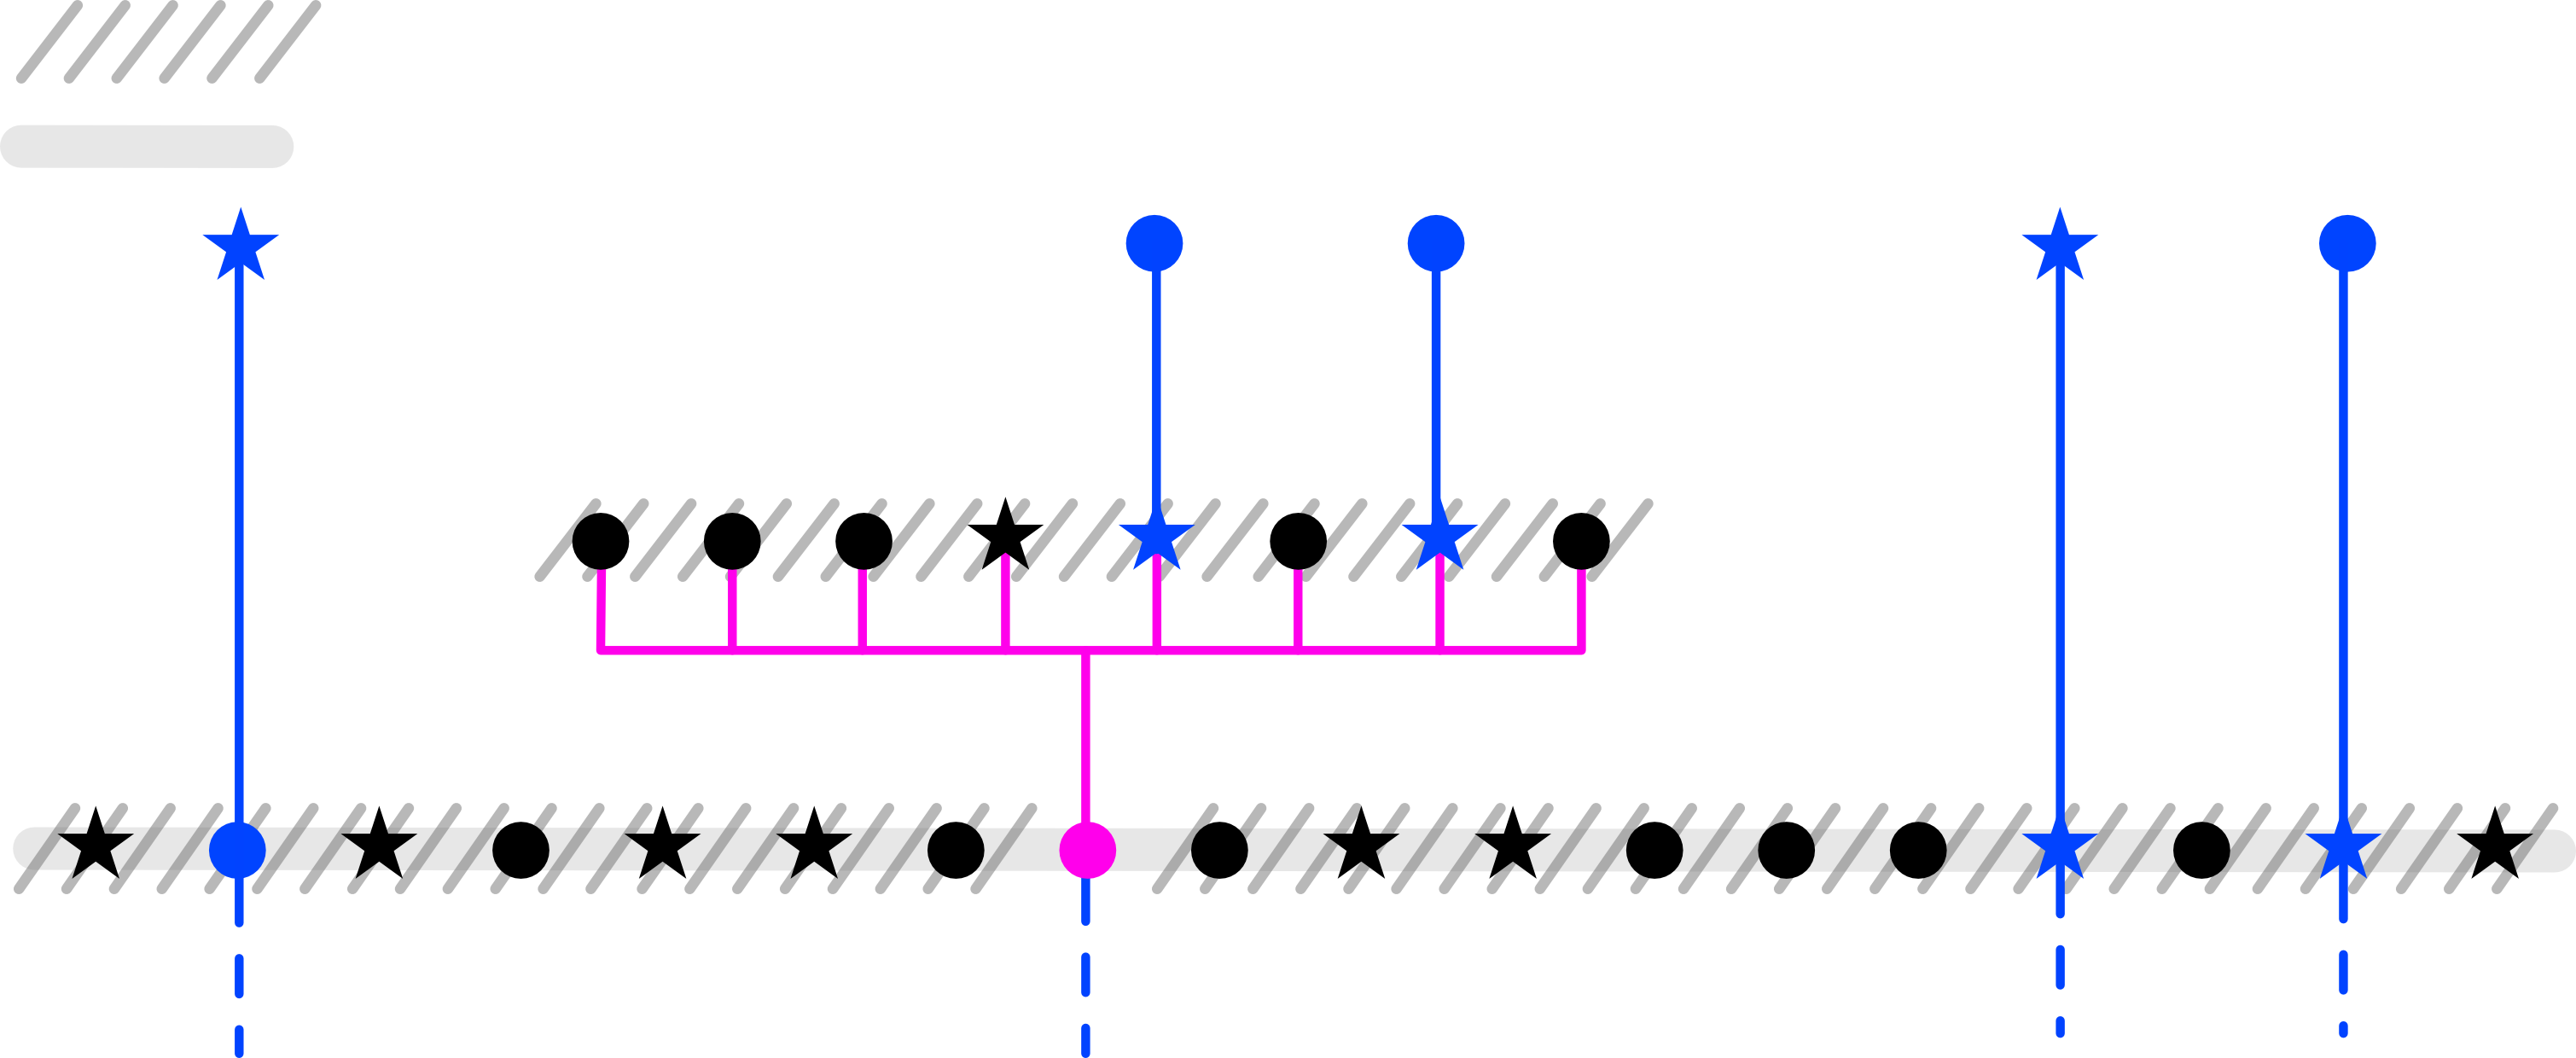
\includegraphics[width=666.75pt,height=258.75pt]{ch4/fig/immigration_genealogies.png}};
%Straight Lines [id:da21468375535797246] 
\draw [line width=3]    (905,339) -- (905,31.06) ;
\draw [shift={(905,23.06)}, rotate = 90] [fill={rgb, 255:red, 0; green, 0; blue, 0 }  ][line width=0.08]  [draw opacity=0] (22.8,-5.7) -- (0,0) -- (22.8,5.7) -- cycle    ;

% Text Node
\draw (116,40) node [anchor=north west][inner sep=0.75pt]    {\Large Population at $t=\theta _{u}^{-}$};
% Text Node
\draw (119,6.4) node [anchor=north west][inner sep=0.75pt]    {\Large Population at $t=\theta _{u}$};
% Text Node
\draw (100,75.4) node [anchor=north west][inner sep=0.75pt]    {\Large$v_{1}$};
% Text Node
\draw (415,72.4) node [anchor=north west][inner sep=0.75pt]    {\Large$v_{2}$};
% Text Node
\draw (513,72.4) node [anchor=north west][inner sep=0.75pt]    {\Large$v_{3}$};
% Text Node
\draw (729,73.4) node [anchor=north west][inner sep=0.75pt]    {\Large$v_{4}$};
% Text Node
\draw (825,73.4) node [anchor=north west][inner sep=0.75pt]    {\Large$v_{5}$};
% Text Node
\draw (88,244.4) node [anchor=north west][inner sep=0.75pt]  [color={rgb, 255:red, 0; green, 0; blue, 0 }  ,opacity=1 ]  {\Large$u_{1}$};
% Text Node
\draw (381,250.4) node [anchor=north west][inner sep=0.75pt]  [color={rgb, 255:red, 0; green, 0; blue, 0 }  ,opacity=1 ]  {\Large$u$};
% Text Node
\draw (717,245.4) node [anchor=north west][inner sep=0.75pt]  [color={rgb, 255:red, 0; green, 0; blue, 0 }  ,opacity=1 ]  {\Large$u_{3}$};
% Text Node
\draw (813,246.4) node [anchor=north west][inner sep=0.75pt]  [color={rgb, 255:red, 0; green, 0; blue, 0 }  ,opacity=1 ]  {\Large$u_{4}$};
% Text Node
\draw (406,144.4) node [anchor=north west][inner sep=0.75pt]    {\Large$w_{1}$};
% Text Node
\draw (502,144.4) node [anchor=north west][inner sep=0.75pt]    {\Large$w_{2}$};
% Text Node
\draw (912.94,72.34) node [anchor=north west][inner sep=0.75pt]  [rotate=-0.52]  {$t$};
% Text Node
\draw (911.97,269.34) node [anchor=north west][inner sep=0.75pt]  [rotate=-0.52]  {\Large$t=\theta _{u}^{-}$};
% Text Node
\draw (911.97,178.34) node [anchor=north west][inner sep=0.75pt]  [rotate=-0.52]  {\Large$t=\theta _{u}$};
% Text Node
\draw (567,194.4) node [anchor=north west][inner sep=0.75pt]    {\Large $\textcolor[rgb]{1,0,0.81}{\mathrm{Ch}(u)}$};



\end{tikzpicture}
   }
    \caption{Illustration of what happens at the first coalescing event for $k=5$ and a population with two types ($E=\{
\bullet,\star\}$). The sampled lineages are pictured in blue, the rest of the population in black. Here, the first coalescing event is characterized by $i=2$ and $d=2$. Forward in time, it corresponds to a branching event at the particle $u$ (in pink). In~\eqref{Ch4:eq:decomposition_first_coal}, we first sample $k-d+1$ particles $\bm u =(u_1,\ldots, u_{k-d+1})$ such that $u_i=u$, then sampling $d$ particles from $\mathrm{Ch}(u)$, then sampling $\bm{v}=(v_1,\ldots, v_k)$ descending from $(u_1,\ldots, u_{i-1}, w_1,\ldots,w_d, u_{i+1}, \ldots, u_k)$. Given the type of the branching particle and the state of the population $(z,\bm x)$ at $\theta_u^-$, the population at $\theta_u$ is given by $z+(L^{(d)}_{x^i}(z,\bm x)-e_{x^i})/K$. The immigration at branching point corresponds to the progeny of $u$ and removing $u$ from the population.}\label{fig:immigration_genealogies}
\end{figure}

\jj{La phrase suivante est bancale: il y a des typos (à relire) et c'est toujours l'histoire de "processus de point" d'un processus de Markov: à reformuler correctement avec la réf que Félix avait trouvée.}
By construction of the model, the jump time of any particle labeled $u$ is given by a the first point of a point process, which intensity measure on $\R_+$ is given by $q_{X^u}(Z_s)ds$.
Thereupon, we integrate the first coalescence time against the jump measure \cite[Theorem~14.2.IV] {daley_vere-jones}. Introducing the compensated integral, it follows that 
\begin{align*}
    & \begin{multlined}[t]  \E_{z}\Big[\Phi_{i,d}\big(\tilde{\Pi}^k_{\cdot,t},  Z^k_t, \bm X^k_t \big)\Big]\  \overset{(\mathrm{C})}{=}\  \frac{k!}{d!(k-d+1)!}\int_0^t \E_{z}\bigg[\frac{\kappa^{k-d+1}_{t-s}(z)}{\kappa^k_{t}(z)} \sum_{u \in\mathcal{N}_{s}} q_{X^u}(Z_s)   \varphi_1(t-s) \\
      \times \frac{(k-d+1)!}{\kappa^{k-d+1}_{t-s}(z)}\sum_{\substack{u_1<\cdots<u_{k-d+1}\in\mathcal{N}_{s}\\ u_i=u}} \varphi_2(\tilde\Pi^{\bm u}_{\cdot, s})m^{(d)}_{X^u}( Z_s, \bm X^{\bm u}_{s})\prod_{j=1}^{k-d+1} H_{X^{u_j}}(Z_{s})   \\
      \times  \E\Big[ \mathcal{M}^k_{t-s}\psi\Big(Z_s+ \frac{L^{(d)}_{X^{u}}(Z_s, \bm X^{\bm u})-e_{X^u}}{K}, \big(\bm X^{\bm u}_{1: i-1}, \bm Y^{(d)}(Z_s,\bm X^{\bm u}),\bm X^{\bm u}_{i+1:k-d+1}\big)\Big)\mid  Z_s,  \bm X^{\bm{u}}\Big]\bigg]ds \end{multlined}\\
       &\overset{(\mathrm{D})}{=}\ \frac{1}{k-d+1}\binom{k}{d} \int_0^t \frac{\kappa^{k-d+1}_{t-s}(z)}{\kappa^k_{t}(z)} \varphi_1(t-s) \
      \E_{z}\Big[ \Phi'_{t-s}\big(\tilde{\Pi}^{k-d+1}_{\cdot,s}, Z^{k-d+1}_{s}, \bm X^{k-d+1}_{s}\big)\Big]ds,
\end{align*}
where $(\mathrm{D})$ comes from recognizing in the second line of $(\mathrm{C})$ the distribution of the random marked planar coalescent $(\tilde{\Pi}^{k-d+1}_{\cdot,s}, Z^k_s,\bm X^{k-d+1}_s)$ introduced in Section~\ref{Ch4:sec:model_formal}, together with the expression of the functional $\Phi'_{t-s}$ from~\eqref{Ch4:eq:functional_pruning}. This finally recovers~\eqref{Ch4:eq:many_to_few_recursion} and completes the proof of Theorem~\ref{thm:many_to_few}
\end{proof}


\begin{rem}[Illustration on monotype, fixed-size models]
Let us illustrate the methodology by drawing a parallel with monotype, fixed-sized population models, whose genealogies have been extensively studied.
Consider the $\Lambda$-Moran model with population size $K$.  This model has been studied for instance in~\citet{etheridge_coalescent_2010,birkner_measure-valued_2009}.
% , in which each individual is further endowed with a genetic type in $E$ that may affect its fitness.
The evolution of the population is given by a resampling mechanism: each $d$-uplet of individuals dies after an exponential holding time with rate $\lambda_d$, one individual of the $d$-uplet is replaced by $d$ copies of themselves.

First, we planarize the problem and affect labels uniformly as described in Section~\ref{Ch4:sec:model_formal}. The $(H,k)$-semigroup does not depend on the population density (which is always equal to $1$), nor on $H$, nor on $\psi$ (since the model is monotype).  In particular, it is a constant of the population state and rewrites
\[
\E\Big[\sum_{\substack{\bm u\in \mathcal{N}_t\\ \forall i,\ u_i\succcurlyeq i}}1 \Big]\ =\ \E\Big[\prod_{i=1}^k Z^{(i)}_t \Big],
\]
where $Z^{(i)}_t$ denotes the proportion of individuals that descend from $i$ in the population at time $t$.

Let $\tilde\Lambda^{k}_{\cdot, t}$ be the $k$-coalescent process giving the genealogies of $k$ individuals sampled at time $t$, which is known to be the (planar) $\Lambda$-coalescent.
We have that
\begin{align*}
\Prob\big(\tau(\tilde\Lambda^{k}_{\cdot, t}) >t\big)\ &=\ \E\Big[\sum_{u_1\neq \ldots \neq u_k}\prod_{i=1}^k Z^{(u_i)}_t \Big]\\
& =\ \exp\Big(-t\sum_{p=2}^k \mbinom{k}{p} \lambda_{k,p}\Big),
\end{align*}
using the moment duality formula. Moreover, for 
\[
\Phi:\tilde\pi_\cdot\ \mapsto\ \1(\tau(\tilde\pi_\cdot ))\phi(\tau(\tilde\pi_\cdot ))\phi_2(\Theta(\tilde \pi_\cdot))\1(\tilde\pi_\tau = \{\{1\},\ldots, \{ i,\ldots, i+d-1\},\ldots,\{k\}\}),\]
replacing in~\eqref{Ch4:eq:many_to_few_recursion}, the semigroup term is deterministic. Getting it out of the expectation, we obtain
\begin{align*}
\E\Big[\Phi(\tilde\Lambda^{k}_{\cdot, t}) \Big]\ &=\ \E\Big[\sum_{u_1\neq \ldots \neq u_k}\prod_{i=1}^k Z^{(u_i)}_t \Big]\\
& =\ \frac{1}{k-d+1}\binom{k}{d}\int_0^t \phi_1(t-s)\E\Big[\phi_2(\tilde\Lambda^{k-d+1}_{\cdot, s})\Big]\exp\Big(-(t-s)\sum_{p=2}^k \mbinom{k}{p} \lambda_{k,p}\Big).
\end{align*}
We recover the recusrive formula obtained by applying the backward Kolmogorov equation in the planar $\Lambda$-coalescent~\citep{Foutel-Rodier:UMS}. Thus, we recover the dirstibution of the planar genealogies from the recursive formula and the dynamics of neutral fractions.
\end{rem}

% {\color{blue}
% \begin{rem}
% Let us illustrate the methodology on population models whose genealogies have been extensively studied. For example, take the $\Lambda$-Moran model. This model has been studied for instance in~\citet{etheridge_coalescent_2010,birkner_measure-valued_2009}, and can be seen as a continuous-time version of Cannings model or a Moran model with several offsprings. As derived in~\cite{etheridge_coalescent_2010}, its infinite population limit is given by a $\Lambda$-Fleming--Viot process, and its dual is the $\Lambda$-coalescent of~\citet{Pitman:1999aa, sagitov1999general}. The coalescence rate of $d$ blocks is given by $\lambda^k_d =\int_0^1 x^{d-2}(1-x)^{k-d}\Lambda(dx)$, $\Lambda$ being a finite measure on $[0,1]$. The total rate of coalescence events when there is $k$ lineages is thus given by $\lambda^k= \sum_{d=2}^k \binom{k}{d} \lambda^k_{d}$.
% The coalescent process from $k$ particles sampled with replacement at time $t$ satisfies
% \[ 
% \Prob\big(\tau(\tilde\Pi) >t\big)\ =\ \exp\Big(-t\sum_{p=2}^k \mbinom{k}{p} \lambda_{k,p}\Big).
% \]
% This formula has the same form as of~\eqref{Ch4:eq:many_to_few_basecase} for  $\Lambda$-Coalescents, with the exponential term corresponding to $\mathcal{M}^k_t\bm{1}(z, \bm x)$. \jj{je comprends pas le lien entre les formules.}
% With the moment duality formula (see~\citet[Lemma~5]{bertoin_stochastic_2003}), we also have that for all $t\geq 0$,
% \[
% \Prob_{N_0=(0,1,\ldots,1)}\big(\tau(\tilde\Pi) > t\big)\ =\  \E_{\bm N_0}\Big[\prod_{i=1}^k (Z^{i}_0)^{N_t^i}\Big] \ =\ \E_{\bm Z_0}\Big[\prod_{i=1}^k Z^{i}_t\Big],
% \]
% \jj{Pas clair le display pour moi...}
% where $N^i_t$ is the block-counting process of lineages in subfamily $i$ and $\bm Z_t: (Z^{0}_t, \ldots, Z^{k}_t)$ are the neutral fractions in the $\Lambda$-Moran model, taking values in the $k+1$-simplex and initialized at $\bm Z_0 : (1-k/K, K^{-1}, \ldots, K^{-1})$. 

% More generally, if we consider the $\Lambda$-coalescent process started from $k$ lineages $\Pi^{\Lambda,k}_t$ \jj{je chipote, mais attention, notation conflictuelle avec la nôtre, ça pourrait aussi perturber}, the backwards Kolmogorov equation~\citep{Ethier:1986uw} yields that 
% \[
% \E_{\pi_0}\big[\Phi(\Pi^{\Lambda,k}_t)\big]\ =\  \sum_{n= 0}^{k-1} \sum_{\bm \pi: \pi_0\to \cdots \to \pi_n} \int_{0< t_1<\cdots < t_n<t}\e^{-\lambda^k t_1} \prod_{j=1}^{n} \lambda_{k_{j-1}, d_j}  \e^{-(t_{j+1}-t_{j})\lambda^{k_j}}\Phi(\pi_n) dt_1\cdots dt_n.
% \]
% If we take the recursive formula of Theorem~\ref{thm:many_to_few} and, anticipating the last section of the article, assume that we can remove the dependence in the total population and iterate~\eqref{Ch4:eq:many_to_few_recursion} through the branching times, we obtain a similar formula.

% \ffr{Pas sûr que ce soit la meilleure place pour parler de ça, on en discute.}\ma{todo voir où inclure cette discussion}
% \end{rem}}

In the remainder of this article, we give an application of the methodology presented in Sections~\ref{Ch4:sec:many_to_few} and~\ref{Ch4:sec:semigroup} to obtain the scaling limit of genealogies in finite type spaces and under Assumption~\ref{hyp:kingman}.
When the space of types is finite and the mean dynamical system~\eqref{Ch4:eq:mean_dynamical_system}
drives the population frequencies to an invariant distribution $\tilde{h}$, we will see that the local stability of the dynamical system allows to choose a sampling function $H$ that simplify the stocastic calculus.
\section{Analysis of the dynamical system}\label{Ch4:sec:katz}
\subsection{Deterministic approximation of neutral fractions}

\ffr{Désolé de faire ce commentaire si tard mais : on a besoin des fractions neutres avec $k$ ? En fait on veut juste définir $H$, donc on peut prendre $k=2$ ce qui simplifie pas mal les notations.}\ma{oui, on a besoin des fractions neutres 'triviales' tq $z^i= e_{x^i}$}

We recall from Proposition~\ref{Ch4:prop:kurtz} that under Assumption~\ref{hyp:kingman}, the population density is well approximated by the deterministic dynamical system $\dot{z}_t = z_t M(z_t)$ in an $\eps$-neighborhood $\mathscr{B}_{\eps}$ of $\tilde h$, where we recall $\eps$ from Assumption~\ref{hyp:kingman}. $\mathscr{B}_{\eps}$ is included in the basin of attraction of $\tilde h$, so that if $z_0\in \mathscr{B}_{\eps}$ then $z_t\in \mathscr{B}_\eps$ for all $t>0$. This system is locally asymptotically stable and drives the deterministic part of the SDE to the stationary profile $\tilde h$.
Moreover, it can be decomposed into $k+1$ parts $z^0_t,\ldots, z^k_t$ such that $z_t=\sum z_t^i$ and
\[
\forall i\in \{0, \ldots, k\},\qquad \dot{z}^i_t \ =\ z^i_t M(z_t).
\]
Intuitively, this amounts to splitting the initial mass into $k+1$ parts and tracking the evolution of each group. Since the growth rate per capita only depends on the total density, the system of differential equations is coupled through $z_t$, solution to~\eqref{Ch4:eq:mean_dynamical_system}.

 If we consider the system of differential equations presented in the above display, we see that any convex combination of $\tilde{h}$ is a stable equilibrium. Thus, the set of convex combinations of $\tilde h$ is a stable manifold for the deterministic part of the system of neutral fractions. 
 Following the notation of~\cite{Julie_Zsofia}, for any initial conditions $z_0$ in $\mathscr{B}_{\eps}$, we write $\phi(t,z_0)$ for the solution at time $t$ to the dynamical sytem~\eqref{Ch4:eq:mean_dynamical_system} with initial condition $z_0$. Then, for $\hat z_0\in\mathscr{B}_\eps$, we introduce  the flow $\hat \phi(t, z_0, \hat z_0)$ to be the the solution at time $t$ to the system
 \[
 \dot{z}_t\ =\ z_t M(\phi(t,z_0)),
 \]
with initial condition $\hat z_0$. 

From there, we define a projection operator.
\begin{propdef}[Katzenberger's projection]
  For any initial subdivision of the population density into $k+1$ parts $\bm z_0=(z_0,z^1_0,\ldots, z^k_0)$ and $i\in\{1,\ldots,k\}$, the projection
  \begin{equation}\label{Ch4:eq:def_katz_proj} 
\theta_i(\bm z_0)\ \coloneqq\ \lim_{t\to\infty} \hat\phi(t, z_0, z^i_0)
\end{equation}
  is well-defined and colinear to $\tilde h$.
\end{propdef}
\begin{proof}
The flow $\phi(t, z_0, z^i_0)$ is solution to
 \[
 \begin{cases}
 \dot{w}_t\ =\ w_t M(\phi(t,z_0)),\\
 w_0\ =\ z^i_0.
 \end{cases}
 \]
 Since $v_0\in \mathscr{B}_{\eps}$ belongs to the basin of attraction of $\tilde h$, the (local) Hartman--Grobman theorem gives that $\phi(t,z_0)$ converges exponentially fast (in norm) to $\tilde h$. The differentiability of the function $z\mapsto M(z)$ gives that $M(\phi(t,z_0))$ converges exponentially fast to $ M(\tilde h)$.
From there, Duhamel's formula gives that

\[
w_t\ =\ \hat z^i_0 \e^{M(\tilde h)t} + \int_0^t w_s\big(M(\phi(s,z_0))-M(\tilde h)\big)\e^{M(\tilde h)(t-s)}ds.
\] 
An application of the Grönwall theorem and the exponential decay of 
$\lVert M(\phi(s,z_0))-M(\tilde h)\rVert$ shows that $(w_t)_t$ is uniformly bounded.
By Assumption~\ref{hyp:PF}, there exists $\lambda, C >0$ such that
\[
\e^{M(\tilde h)t}\ =\ h^\transpose\tilde h+ R_t\quad \textit{with} \quad \lVert R_t\rVert\ \leq \ C\e^{- \lambda t},
\]
so that the first term in the above display converges to $\langle \hat z^i_0, h \rangle \tilde h$. Besides, 
the integral rewrites as 
\[
\int_0^t \langle w_s \big(M(\phi(s,z_0))-M(\tilde h)\big), h \rangle\tilde h + \int_0^t w_s \big(M(\phi(s,z_0))-M(\tilde h)\big)R_{t-s},
 \]
the first part being absolutely convergent and colinear to $\tilde h$, and the second part vanishes using the exponential decay of $R_{t-s}$.

 Thus, the $(\theta_i(\bm z_0))_{i\leq k}$ exists and are colinear to $\tilde h$, so that the projections $\theta_1(\bm z_0),\ldots, \theta_k(\bm z_0)$ from~\eqref{Ch4:eq:def_katz_proj} belong to the stable manifold of the system~\eqref{Ch4:eq:mean_dynamical_system}.
\end{proof}
 The projections from~\eqref{Ch4:eq:def_katz_proj} are called \emph{Katzenberger projections} in~\cite{Julie_Zsofia}.
In a more general setting,~\cite{Katzenberger:1991aa} proved a dimension reduction result in this slow-fast parameter regime. They proved that once time-changed to observe the stochasticity, the system converges to a reduced SDE forced onto the stable manifold of the deterministic system. In the case of a $E\times (k+1)$-dimensional system whose stable manifold is the compact subset given by $\Delta^k \tilde h$, where $\Delta^k$ is the simplex 
\[ \Delta^k\ \coloneqq\ \Big\{(u^0,\ldots, u^{k+1})\in \R_+^{n+1},\  \sum_{i=0}^k u^{i}=1\Big\},\] 
the theory of~\cite{Katzenberger:1991aa} allows to approximate the dynamics with a SDE on scalar projection. 

In general, the expressions of this so-called Katzenberger projection and those of the coefficients of the reduced SDE are not explicit.
However, in the case of stable SDEs such that their structure is infinitely divisible (that is typically the case of infinite-population limit of individual-based models),~\citet{Julie_Zsofia} proved that the structure of neutral fractions allows for a linear form representation of the projection. They started from a limiting SDE model with the so-called \emph{infinitely decomposable} property, meaning that the population can be subdivided into as many  sub-populations as one wants.
However the deterministic dynamical system is the same,  so that the same proof holds for our individual-based model. 
 More formally, we have the following Lemma~\ref{lem:proj_katz_H}, which corresponds to~\citet[Proposition~7]{Julie_Zsofia}.
 \begin{lem}[Riesz representation of the projection]\label{lem:proj_katz_H}
There exists a positive function
\[
\begin{aligned}
H:\  E\times \mathscr{B}_{\eps}\ &\longrightarrow\ \R^*_+\\
 (x, z)\ &\longmapsto\ H_x(z),
\end{aligned}
\]
such that for all $i\leq k$ and $\bm z=(z^1,\ldots, z^k)$ satisfying $z=\sum_j z^j\in \mathscr{B}_{\eps}$, the $i^{th}$ Katzenberger
projection defined in~\eqref{Ch4:eq:def_katz_proj} is given by
\[\theta^i(\bm Z_t)\ \coloneqq\ \langle  Z_t^{i}, H( Z_t)\rangle \tilde h,\] 
rewriting as a linear projection of the neutral fraction $ Z_t^{i}$. 
 \end{lem}
 \begin{proof}
 We refer to \citet[Proposition~7]{Julie_Zsofia} for the proof.
 \end{proof}
We see from Lemma~\ref{lem:proj_katz_H} that the function $H$ plays the same role as the harmonic function $h$ in the branching setting. Thus, it can be interpreted as a \textit{dynamical reproductive value}.

\begin{rem}
Taking the unstructured (single type) model from~\cite{AFRS_2025}, the scalar dynamical system~\eqref{Ch4:eq:mean_dynamical_system} re-writes 
\[ \dot z_t\ =\ z_t q(z_t)\big(m(z_t)-1\big),\]
where $m(z)\coloneqq \E[L(z)]$. 
Computing~\eqref{Ch4:eq:def_katz_proj} for $z_0,\hat z_0$ in the basin of attraction of $1$, 
\[
\hat\phi(t,z_0,\hat z_0)= \hat z_0\exp\Big(\int_0^t q(z_s)(m(z_s)-1)ds\Big)\ =\ \hat z_0 \frac{\phi(t,z_0)}{z_0},
\]
which in the limit yields $\theta_{i}(z)=z^i/z$, so that in the single type setting, the Katzenberger projection is the inverse function
\[
H: z\ \longmapsto\ \frac{1}{z}.
\]
\end{rem}


\subsection{Properties of the dynamical reproductive value}\label{Ch4:sec:katz_properties}
In this paragraph, we recall from~\cite{Julie_Zsofia} the properties of the dynamical reproductive value, and some key identities which will be useful in the proof of our main result.
To begin with, adapting the result of~\citet[Lemma~10, Appendix~C]{Julie_Zsofia} to the case where the limiting dynamical system is only two times differentiable, we have the following regularity result on $(x,z)\mapsto H_x(z)$.
\begin{lem}
$H$ is twice continuously differentiable in a neighborhood of $\tilde{h}$.
\end{lem}
\begin{proof}
The result comes from the local $\mathcal{C}^2(\R^E, \R^{E\times E})$ regularity of the mean matrix $z\mapsto M(z)$ stated in Assumption~\ref{hyp:stability}. We refer to~\citet[Lemma~10, appendix~C]{Julie_Zsofia} for the proof of this result.
\end{proof}
Up to taking a smaller $\eps$, we assume that $H$ is three continuously differentiable on $\mathscr{B}_{\eps}$.

\begin{lem}[Extension of $H$ on $\R_+^E$]\label{lem:H_outside_domain_attraction}
Outside of $\mathscr{B}_{\eps}$ we can define $H$ in a way to ensure that 
\begin{itemize}
\item $H$ coincides with the dynamical reproductive value from Lemma~\ref{lem:proj_katz_H} on $\mathscr{B}_{\eps}$;
\item $H$ is $\mathcal{C}^2$ on $\R_+^E$;
\item $H$ is positive coordinate-wise;
\item $H$ and $\langle z, H(z)\rangle$ are bounded.
\end{itemize}
\end{lem}
\begin{proof}
  The function $H$ from Lemma~\ref{lem:proj_katz_H} is $\mathcal{C}^2$ on the compact $\mathscr{B}_{\eps}$. Thus, the  Whitney extension theorem provides an extension $\tilde H$ such that  $\tilde H$  is twice continuously differentiable on $\R_+^E$ and 
  \[
 \forall z\in\mathscr{B}_{\eps},\quad \tilde H(z)\ =\ H(z).
  \]
  From there, we construct a smooth cutoff of $\tilde H$ to satisfy the last two points.
  
  Since $H$ is coordinate-wise positive and continuous on the compact ball $\mathscr{B}_{\eps}$, it attains a positive minimum
\[ H_{\min} \coloneqq\ \min_{x\in E}\ \min_{ \mathscr{B}_{\eps}} H_x(\cdot )\ >0 .
\]
By continuity of the extension $\tilde H$, there exists $\eps'>0$ such that $\tilde H(z)> H_{\min}/2$ for all $z\in\mathscr{B}_{\eps +\eps'}$.



  Let $\alpha_: t\longmapsto \exp(-1/t)\1(t>0)$ be a decaying function, and consider the function
  \[
\beta: t\ \longmapsto\ 1- \frac{\alpha(t)}{\alpha(t)+\alpha(1-t)},
  \]
  such that $\beta \equiv 1$ on $(-\infty, 0]$ and $\beta \equiv 0$ on $[1,\infty)$,
and
\[
\phi: z\ \longmapsto\ \beta\Big(\frac{\lVert z- \tilde h\rVert - \eps}{\eps'}\Big)\ \in\ [0,1],
\]
  with $\varphi\equiv1$ on $\mathscr{B}_\eps$ and $\varphi\equiv0$ outside $\mathscr{B}_{\eps+\eps'}$.
  From there, we define the extension $\hat H$ for all $z\in\R_+^E$ as
  \[
  \hat H(z)\ \coloneqq\ \phi(z)\tilde H(z) + (1-\phi(z))\frac{1}{1+\lVert z\rVert^2}.
  \]
  We easily check that $\hat H$ is potitive coordinate-wise and that $\langle z, H(z)\rangle$ is bounded. Moreover, $\hat H$ is $\mathcal{C}^2$ by product and sum.
\end{proof}


Moreover by construction in~\eqref{Ch4:eq:def_katz_proj} and Lemma~\ref{lem:proj_katz_H}, the Katzenberger projections onto $H$ remains constant under the action of the flow field of the deterministic dynamical system. That is, for all initial population $z\in \mathscr{B}_\eps$, we have that 
\begin{equation}\label{Ch4:eq:katz_proj_is_one}
\langle z, H(z)\rangle\ =\ 1.
\end{equation}
Moreover, for all decomposition in fractions $(z^i)_{0\leq i\leq k}\in \R_+^E$ such that $z=\sum_i z^i\in\mathscr{B}_\eps$, if $z_t=\sum_{i}z^i_t$ is solution of the mean dynamical system~\eqref{Ch4:eq:mean_dynamical_system} and $z_t^i$ has initial condition $z^i$, we have that for all $t\geq 0$,
\begin{equation}\label{Ch4:eq:katz_identity_flow}
\langle z^i_t, H(z_t)\rangle\ =\ \langle z^i, H(z)\rangle.
\end{equation}
Recall the Perron-Frobenius eigenvectors $h$ and $\tilde h$.
In particular for $z_0= \tilde h$, we have by definition that
\[
 \phi(t, \tilde h )\ =\ \tilde h \exp\big(M(\tilde h)t\big),
\]
so that letting $t\to\infty$, we have for any initial neutral fraction $\hat{z}_0$ that
\begin{align*}
\langle \hat z_0, H(\tilde h)\rangle\tilde h\ &=\ \lim_{t\to \infty} \exp\big(M(\tilde h)t\big)\hat z_0\\
& =\ \langle \hat z_0, h\rangle \tilde h ,
\end{align*}
which yields $H(\tilde h) = h$.
This implies that there exists a neighborhood of $\tilde h$ in which $H(z)$ is positive coordinate-wise. Once again up to taking a smaller $\epsilon$, we assume that $H$ is positive on $\mathscr{B}_{\eps}$.

The key identities that will be used in the computational section are that stated in the following Lemma~\ref{lem:properties_katz}, which we recall from~\cite{Julie_Zsofia}.
\begin{lem}{\cite[Lemma~12]{Julie_Zsofia}}\label{lem:properties_katz}
For all $y\in E$ and $z\in \mathscr{B}_\eps$, it holds coordinate-wise that
\begin{equation}\label{Ch4:eq:katz_identity}
\sum_y z_y \nabla H_y(z)  + H(z)\ =\ 0, \qquad
\sum_y z_y  \nabla^2 H_y(z)\rangle + \nabla H(z)+ \nabla H(z)^{\transpose}\ =\ 0,
\end{equation}
where $\nabla H(z)$ is the matrix with coordinates $\big(\partial_x H_y(z)\big)_{x,y\in E}$.
Moreover, for all $x\in E$,
\begin{equation}\label{Ch4:eq:regle_calcul_katz}
  \big\langle e_{x} M(z), H(z)\big\rangle +  \big\langle\nabla H_{x}(z), zM(z)\big\rangle = 0.
\end{equation}

% \begin{multline}
%    \sum_{x\in E,j\leq k} \big(\nabla \langle z^i, H(z) \rangle \big)_{x,j}\big( M (z )z^j\big)_x\ = \sum_{x \in  E} \Big[H_x(z)\big( M (z )z^i\big)_x + \sum_{j= 0}^k \langle z^i, \partial_x H(z) \rangle \big( M (z )z^j\big)_x  \Big]\\
%    =\  \sum_{x \in  E} \Big[H_x(z)\big( M (z )z^i\big)_x +  \langle z^i, \partial_x H(z) \rangle \big( M (z )z\big)_x  \Big] =\ 0,
% \end{multline}
\end{lem}
\begin{proof}
The identity~\eqref{Ch4:eq:katz_identity} simply comes from differentiating the identity~\eqref{Ch4:eq:katz_proj_is_one} 
in the directions $(e_x)_x$. 

Let $z^0,\ldots, z^k$ such that $z=\sum_{j=0}^k z^j$. Differentiating~\eqref{Ch4:eq:katz_identity_flow} with respect to time yields that
for all $i\in\{1,\ldots, k\}$,
\[
\langle \dot{z}^i_t, H(z_t)\rangle + \langle z^i_t, \nabla H(z_t)\dot{z}_t\rangle \ =\ \langle z^i_t M(z_t), H(z_t)\rangle + \langle z^i_t, \nabla H(z_t)\cdot z_tM(z_t)\rangle\ =\ 0.
\]
Evaluating at $t=0$, we obtain
\[
\sum_{x,y\in E}z^i_x \partial_y H_x(z) (zM(z))_y + \langle z^i M(z), H(z)\rangle\ =\ 0.
\]
From there~\eqref{Ch4:eq:regle_calcul_katz}comes from taking the subfamily $z^i=e_x$.
\end{proof}


In the following sections, we choose $H$ to be the sampling function in the construction of the marked planar coalescent of Section~\ref{Ch4:sec:model_formal}.
For $(z,\bm x)\in\R_+^E\times E^k$. We recall the notation $\mathcal{H}(z,\bm x)=\prod_{i=1}^k H_{x^i}(z)$.
By~\eqref{Ch4:eq:katz_proj_is_one} and Lemma~\ref{lem:H_outside_domain_attraction}, we have that for all $\bm x\in E^k$,
$\mathcal{H}(\,\cdot\, ,\bm x)$ is bounded on $\R_+^E$. Moreover, the regularity of the Katzenberger projection and its extension to $\R_+^E$ constructed in Lemma~\ref{lem:H_outside_domain_attraction} give that $\mathcal{H}(\,\cdot\, , \bm x)$ is $\mathcal{C}^2$ on $\R_+^E$. 

\section{Heuristics for the proof of Theorem~\ref{thm:main_multitype}}\label{Ch4:sec:heuristics}
The remainder of this article is dedicated to the proof of Theorem~\ref{thm:main_multitype}.
In order to guide the reader through the proof, we will begin with some heuristic arguments to shed some light on the roadmap we will follow in Section~\ref{Ch4:sec:calcul_sto} and Section~\ref{Ch4:sec:convergence} to prove Theorem~\ref{thm:main_multitype}.
\subsection{Concentration of the $(H,k)$-spine process}\label{Ch4:sec:heuristics_concentration}

For all $k\geq 0$, we recall the spinal process $(\mathcal Z^k_s,\bm S^k_s)_{s\geq 0}$ from Definition~\ref{def:spine_one_particle_per_family}, with the convention that $k=0$ corresponds to the initial density process $(Z_s)_{s\geq 0}$ and no spines.
Recall the parameter $\eps$ from Assumption~\ref{Ch4:eq:UI_moment}. For all $\gamma\in (0,\eps)$, denote by $\mathscr{B}_{\gamma}$ the ball with radius $\gamma$ and centered in $\tilde h$. Denote by $T_{\gamma}$ the stopping time
\begin{equation*}
      T_{\gamma} \ \coloneqq\ \inf\big\{t\geq 0,\ \lVert \mathcal{Z}^k_t-\tilde h\rVert > \gamma \big\}.
\end{equation*}

In the proof of Theorem~\ref{thm:main_multitype}, we will rely on the concentration results from Proposition%~\ref{Ch4:prop:coupling},
~\ref{Ch4:prop:total_popsize} and Proposition~\ref{Ch4:prop:cv_spinaltypes}, that formalize the averaging of the ecology of the spinal particle process to a stationary distribution on the evolutionary timescale $O(K)$ on which coalescing events occur in the $(H,k)$-coalescent.

\begin{prop}[Convergence of the population density]\label{Ch4:prop:total_popsize}
 For all $k\geq 0$,  $T>0$, $\gamma>0$, $\bm x\in E^k$ and sequence of initial conditions $(z_K)_K$ satisfying that $\lVert  z_K-\tilde h\rVert\to 0 $ as $K\to\infty$, we have
\begin{equation*}
    \mathbb{P}_{z_K,\bm x}\big(T_{\gamma}<KT\big)\ \underset{K\to\infty}{\longrightarrow}\ 0. 
\end{equation*} 
\end{prop}
Proposition~\ref{Ch4:prop:total_popsize} states that the for every $k\geq 0$, the density of the $(H,k)$-spine process converges to its equilibrium. In particular for $k=0$, it is an extension of the concentration result derived by~\cite{Kurtz:1978aa} for density-dependent particle systems on compact time intervals (see Proposition~\ref{Ch4:prop:kurtz}) to the timescale $O(K)$.
 
\begin{prop}[Convergence of types along the spines]\label{Ch4:prop:cv_spinaltypes}
Let $k\geq 1$, $t > 0$, $\bm x\in  E^k$. For any sequence of initial population density  $(z_K)_K$ satisfying that $z_K \to \tilde h$ as $K\to\infty$, the distribution of $\bm{S}^k_{Kt}$ converges to $(h\tilde h)^{\otimes k}$ as $K\to\infty$.

That is, for every $\bm y = (y^1,\ldots, y^k)\in E^k$, we have the convergence
\begin{equation}\label{Ch4:eq:cv_types}
 \lim_{K\to\infty }\Prob_{z_K,\bm x}\big(\bm S^k_{Kt} =\bm y\big)\ =\ \prod_{i=1}^k h_{y^i}\tilde h_{y^i},
\end{equation}
where we recall that for all $t\geq 0$, $S^i_{t}$ denotes the type of the $i^{th}$ spine at time $t$.
\end{prop}


The proof of Proposition \ref{Ch4:prop:cv_spinaltypes} goes along the following lines. From the transitions of $(\bm S^k_t)_{t}$ described in Definition~\ref{def:spine_one_particle_per_family}, the evolution of types on the $k$ spinal lineages is not a Markov chain. In particular it depends on the density process $(\mathcal Z^k_t)_t$. However, motivated by the concentration result in Proposition \ref{Ch4:prop:total_popsize}, if we fix $(\mathcal Z^k_t)_t$ to $\tilde h$, it becomes a continuous-time homogeneous Markov Chain with transitions rates  
\begin{equation*}
 \frac{M(\tilde h)_{x,y}h_y}{h_x},\quad \forall  x, y\in E.
\end{equation*}
  Using the Perron--Frobenius Assumption~\ref{hyp:PF}, we easily check that $(h_x\tilde h_x)_x$ is the stationary probability distribution of this Markov chain.

  \medskip

  

% By Lemma~\ref{lem:coupling_capped}, without loss of generality, we can work with a population process such that $\forall x\in E$, $z\notin \mathscr{B}_{\gamma}\Rightarrow q_x(z)=0$ and $\lVert L_x(z)\rVert \leq \Gamma_K$.
The formal proofs of these two results are computational and not very enlightening to understand the conceptual ideas behind Theorem~\ref{thm:main_multitype}. For this reason, we chose to postpone the formal proofs of Proposition~\ref{Ch4:prop:total_popsize} and Proposition~\ref{Ch4:prop:cv_spinaltypes} to Section~\ref{Ch4:sec:calcul_sto} (see Section~\ref{Ch4:sec:cv_pop} for the proof of Proposition~\ref{Ch4:prop:total_popsize} and Section~\ref{Ch4:sec:cv_spine} for that of Proposition~\ref{Ch4:prop:cv_spinaltypes}). We assume these results hold in the remainder of this heuristics section.  
\subsection{Convergence of the $(H,k)$-semigroup}\label{Ch4:sec:heuristics_section_6}


% In particular, since we are working on the timescale $KT$, Proposition~\ref{Ch4:prop:total_popsize} allows to work with offspring distributions $(L_x(z),\ x\in E,\ z\in \R_+^E)$ such that  \jj{Il n'y a pas de $\Gamma_K$ dans la Proposition~\ref{Ch4:prop:total_popsize}, mais je suis d'accord avec Félix de mettre le lemme dans la section technique plus tard, donc d'enlever carrément toute mention de $\Gamma_K$.}
% \begin{equation}\label{Ch4:eq:bound_as_coupling}
% \sup_{z\in \mathscr{B}_\eps, x\in E}\lVert L_x(z) \rVert \leq 2\Gamma_K\quad \textit{a.s.},
% \end{equation}
% without loss of generality. We will formalize this using a coupling in Section~\ref{Ch4:sec:calcul_sto}.

% The idea is to show that, because of the fast ecological dynamics and the projection on the dynamical reproductive value $H$, the interactions and the movement in the type space average out on the . \ffr{pas très précis "l'écologie de la population se moyenne" : qu'est-ce que tu veux dire ? "la projection sur la valeur repro", c'est la valeur repro qui est une projection non ?.}

The next step will be to show the following Proposition~\ref{Ch4:prop:estimation_feynman-kac}.


\begin{prop}[Convergence of the $(H,k)$-semigroup]\label{Ch4:prop:estimation_feynman-kac}
Let $k,t\geq 0$, $\psi:\R_+^{E}\times E^k$ bounded and such that for all $\bm x\in E^k,$ $z\mapsto \psi(z,\bm x)$ is continuous at $\tilde h$. Then for all $\bm x\in E^k$ and sequence $(z_K)_K\in(\R_+^E)^{\N}$ such that $z_K\to \tilde h$ with $K\to\infty$, 
\begin{equation*}
\lim_{K\to\infty}\mathcal{M}^k_{Kt}\psi( z_K,  \bm x)\ =\ \exp\Big(- \mbinom{k}{2} \bar m_2 t\Big) \sum_{\bm y\in E^k}\psi\big(\tilde h, \bm y \big)\prod_{i=1}^k h_{y^i}\tilde h_{y^{i}}.
\end{equation*}
\end{prop}


The proof of Proposition~\ref{Ch4:prop:estimation_feynman-kac} will be made rigorous in Section~\ref{Ch4:sec:convergence_semigroup}, but we give some heuristic arguments below.

 Let $\bm x\in E^k$ and $(z_K)_K\in (\R_+^E)^{\N}$ be a sequence of initial conditions such that $z_K\to \tilde h$ as $K\to\infty$. By Proposition~\ref{Ch4:prop:P_semigroup_feyman_kac}, we have the following Feynman--Kac representation of the semigroup $\mathcal{M}^k_t$, for all $k,t\geq 0$:
\begin{equation}
\mathcal{M}^k_{Kt}\psi( z_K,  \bm x)\ =\ \E_{z, \bm x}\bigg[\psi(\mathcal{Z}^k_{Kt}, \bm S^k_{Kt})\exp\Big(\int_0^{Kt}\mathcal{G}^k\bm{1}(\mathcal{Z}^k_{s}, \bm S^k_s)ds\Big)\bigg], \label{Ch4:eq:semi-group2}
\end{equation}
where we recall that $\mathcal{G}^k$ is the generator of the $(H,k)$-semigroup from Definition~\ref{def:def_P_semigroup}.
From the definition of $({\cal M}^{k}_t)_{t\geq0}$ and the 
transitions rates of the underlying interacting particle system, one can easily show the following lemma, that we state without a proof.

\begin{lem}\label{lem:generator_applied_to_1}
Let ${\cal G}^k$ be the generator of $({\cal M}^{k}_t)_{t\geq0}$. Then 
\begin{align*} 
K\mathcal{G}^k\bm{1}(z,\bm x)\ &=\  K^2\sum_{y\in E}q_{y}(z) z_y  \E\bigg[\frac{ \mathcal{H}\big(z+ \frac{L_y(z) -e_{y}}{K},\bm x\big)}{\mathcal{H}(z, \bm x ) } - 1\bigg] \\\ 
+\   K &\sum_{i=1}^k  q_{x^i}(z)\E\bigg[\frac{\big\langle L_{x^i}(z) -e_{x^i}, H\big(z+ \frac{L_{x^i}(z) -e_{x^i}}{K} \big)\big\rangle}{H_{x^i}\big(z+ \frac{L_{x^i}(z) -e_{x^i}}{K}\big)}\frac{ \mathcal{H}\big(z+ \frac{L_{x^i}(z) -e_{y}}{K},\bm x\big)}{\mathcal{H}(z, \bm x ) } \bigg].
\end{align*}
\end{lem}
For all $z\in \R_+^E$ and $y\in E$, we denote by $C_y(z)$ the matrix defined for all $x,x'\in E$ by
\begin{equation}\label{Ch4:eq:def_Sigma_covariance}
 C_y(z)\big|_{x,x'}\ \coloneqq\ q_y(z)\E\Big[\big(L_{yx}(z)-\1_{y=x}\big)\big(L_{yx'}(z)-\1_{y=x'}\big)\Big],
\end{equation}
so that the matrix $C_y(z)$ is the symmetric matrix giving the rates at which a single particle with type $y$ contributes to the compensator of the quadratic covariation of the population vector generated by type $y$ individuals in a population with density $z$. Then, we denote by $\bar{C}(z)$ the matrix
\begin{eqnarray*}
\bar{C}(z)\ \coloneqq\ \sum_{y \in E} z_y C_y(z).
\end{eqnarray*}
As $K\to\infty$, we can Taylor expand the expression $K\mathcal{G}^k\bm{1}(z,\bm x)$
around any fixed point $z$. A close inspection of the latter expression suggests that 
\begin{align*}
&K\mathcal{G}^k\bm{1}(z,\bm x)\ =\  K\sum_{i=1}^k\frac{1}{H_{x^i}(z)}\Big(\langle e_{x^i},\nabla H(z)\cdot zM(z)\rangle + \langle e_{x^i}M(z), H(z)\rangle\Big)  \\\label{Ch4:eq:term_antidiag}\tag{$\mathrm{ADg}$}
 & +\ 
\sum_{\substack{i,j=1 \\ i\neq j}}^k\frac{1}{H_{x^i}(z)H_{x^j}(z)} \bigg[ \frac{1}{2}  \big\langle \nabla H_{x^i}(z) ,\bar C(z) \nabla H_{x^j}(z)\big\rangle 
+ \big\langle H(z), C_{x^i}(z) \nabla H_{x^j}(z)\big\rangle \bigg]
\\\label{Ch4:eq:term_diag}\tag{$\mathrm{Dg}$} &
+\ \sum_{i=1}^k\frac{1}{H_{x^i}(z)}\mathrm{Tr}\Big(
  \frac{1}{2} \nabla^2 H_{x^i}(z) \bar C(z)
  +  \nabla H(z)  C_{x^i}(z)\Big)\\
  &+\  o(1),
\end{align*}
where $\mathrm{Tr}(A)$ denotes the trace of a matrix $A$ and $\nabla H(z)$ is the matrix with entries $(\partial_x H_y(z))_{x,y\in E}$.

Thanks to our choice of sampling function $H$ (dynamical reproductive value -- see Section \ref{Ch4:sec:katz}),  the identity (\ref{Ch4:eq:regle_calcul_katz}) implies that that first term of order $K$ vanishes, 
which only leaves us with a term of order~$1$.


For all $z\in \R_+^E$, we introduce the vector $\overline{\nabla H}(z)$ and the matix $\overline{\nabla^2 H}_x(z)$, defined by
\begin{equation}\label{Ch4:eq:bar_nabla_H}
\overline{\nabla H}(z)\ \coloneqq\ \sum_{y \in E} z_y \nabla H_{y}(z)\quad\textit{and}\quad \overline{\nabla^2 H}(z)\ \coloneqq\ \sum_{y \in E} z_y \nabla^2 H_y(z).
\end{equation}

Using the the concentration results and an ergodic theorem, we will show in the next subsection (see Section~\ref{Ch4:sec:convergence_semigroup}) that  
\[ \int_0^{Kt}\mathcal{G}^k\bm{1}(\mathcal Z_s,\bm S^k_{s})ds \ \approx\ t\cdot \sum_{\bm x\in E^k}K\mathcal{G}^k\bm{1}(\tilde h, \bm x)\prod_{i=1}^k h_{x^i}\tilde h_{x^i}\]
Integrating the diagonal term (\ref{Ch4:eq:term_diag}) over the stationary distribution together with~\eqref{Ch4:eq:bar_nabla_H}, we obtain that
\[
 \sum_{i=1}^k\frac{1}{H_{x^i}(\tilde h)}\mathrm{Tr}\Big(
  \frac{1}{2} \nabla^2 H_{x^i}(\tilde h) \bar C(\tilde h)
  +  \nabla H(\tilde h)  C_{x^i}(\tilde h)\Big)\ \approx\ k \mathrm{Tr}\Big(\frac{1}{2} \overline{\nabla^2 H}(\tilde h) \bar C(\tilde h)
  +  \nabla H(\tilde h)\bar C(\tilde h)\Big),
\]
recalling the notation from~\eqref{Ch4:eq:bar_nabla_H}.
From~\eqref{Ch4:eq:katz_identity}, we have that 
\[
\overline{\nabla^2 H}(\tilde h) \ =\ -\big(\nabla H(\tilde h)+ \nabla H(\tilde h)^{\transpose}\big),
\]
so that, using the symmetry of the matrix $\bar C(\tilde h)$ and the invariance of the trace by commutation and transposition, the diagonal term~\eqref{Ch4:eq:term_diag} vanishes in the large $K$ limit.

Finally,
integrating over the anti-diagonal term~\eqref{Ch4:eq:term_antidiag} and
the identity $H(\tilde h)=h$,  
we have
\begin{align*}
 \sum_{\bm x\in E^k}G(\tilde h, \bm x)\prod_{i=1}^k h_{x^i}\tilde h_{x^i}\
 &=\  k(k-1)\Big( \frac{1}{2} \big\langle \overline{\nabla H}(\tilde h), \bar C(z) \overline{\nabla H}(\tilde h)\big\rangle + \big\langle h, \bar C(z) \overline{\nabla H}(\tilde h)\big\rangle\Big)\\
&=\ -\frac{k(k-1)}{2}\big\langle  h,  \bar C(\tilde h) h\big\rangle \\
& =\ -\binom{k}{2}\bar m_2,
\end{align*}
where we used that, from~\eqref{Ch4:eq:katz_identity}, we have that $\overline{\nabla H}(\tilde h) = - h$.


\subsection{Convergence of the $(H,k)$-coalescent}
\label{Ch4:sec:heuristics_many_to_few}

Finally, we explain with heuristic arguments how we wrap up the proof of Theorem~\ref{thm:main_multitype} from the results in Section~\ref{Ch4:sec:heuristics_concentration} and Section~\ref{Ch4:sec:heuristics_section_6} and the recursive formula given in Theorem~\ref{thm:many_to_few}. The formal proofs are developed in Section~\ref{Ch4:sec:fin_preuve}. The main result of this section is given in Proposition~\ref{Ch4:prop:cv_moments_planaires}.



We define the planar $k$-Kingman coalescent with rate $\bar{m}_2>0$ as the planar $k$-coalescent $(\tilde{\mathcal{K}}^k_{s})_{ s\geq 0}$ with binary mergers and the following transition dynamics.
It starts from the singleton partition $\{\{1\},\ldots,\{k\}\}$ and, when there are $p$ blocks, any pair of \textit{adjacent blocks} merges at rate $p \bar{m}_2 / 2$.
We endow the blocks with marks distributed independently and according to the stationary measure of the spine $h\tilde h$.


\begin{prop}[Scaling limit of the $(H,k)$-planar coalescent]\label{Ch4:prop:cv_moments_planaires} 
  
  Let $k\geq 1$, $t>0$
and let $(z_K)_K$ be a deterministic sequence of initial conditions in $\R_+^E$ satisfying that $z_K\to \tilde h$
    as $K\to\infty$. Then, the following limit holds in distribution: 
    \begin{equation}\label{Ch4:eq:def_limit_measure}
        \lim_{K\to\infty}\  
         \big((\tilde{\Pi}^k_{Ks,Kt})_{s\in[0,t]},\, Z^k_{Kt},\, \bm X^k_{Kt}\big)
        \ = \   
       \big((\tilde{\mathcal{K}}^{k}_{s})_{s\in[0,t]},\, \tilde h,\, \bm X \big),
    \end{equation}
    where $\bm X\sim (h\tilde h)^{\otimes k}$, and $\tilde{\mathcal{K}}^k_\cdot$ is a planar $k$-Kingman coalescent with rate $\bar{m}_2$ independent of $\bm{X}$.
\end{prop}

The proof of this result is the main matter of Section~\ref{Ch4:sec:fin_preuve}.    Once again, we give some heuristics towards the proof of Proposition~\ref{Ch4:prop:cv_moments_planaires}.


First, for $k\geq 2$ we observe that Proposition~\ref{Ch4:prop:cv_moments_planaires} is equivalent to proving that the $(H,k)$-spine process converges to $(\tilde h,\bm X)$ with $\bm X\sim (h\tilde h)^{\otimes k}$ on the timescale $O(K)$ (which is already given by the concentration results stated in Section~\ref{Ch4:sec:heuristics_concentration}) and that there exists a limiting planar $k$-coalescent with binary mergers which satisfies the recursive formula~\eqref{Ch4:eq:limit_recurrence}, characterizing the distribution of the planar $k$-Kingman coalescent with rate $\bar m_2$.
    \begin{equation}\label{Ch4:eq:limit_recurrence}
    \begin{dcases}
        \Prob\Big(\tau\big(\tilde{\mathcal{K}}^k_\cdot\big)>t\Big) \ =\ 
       \exp\Big(-\bar m_2\mbinom{k}{2}t\Big) \\
       \E\Big[\Phi\big(\tilde{\mathcal{K}}^k_\cdot\big)\Big]\ =\  \int_{0}^{t}\varphi_1(t-s)
        \E\Big[\varphi_2\big(\tilde{\mathcal{K}}^{k-1}_\cdot\big)\Big] \frac{\bar m_2}{k-1}\binom{k}{2}
        \exp\Big(-\bar m_2\mbinom{k}{2}(t-s)\Big) d s,
    \end{dcases}
    \end{equation}
    for every $\Phi$ of the following product form: 
    \begin{multline*}
 \Phi(\tilde \pi_{\cdot} )\ \coloneqq\ \1\big(0<\tau(\tilde \pi_{\cdot} )<t\big) \cdot \varphi_1\big(\tau(\tilde \pi_{\cdot} )\big)\cdot  \varphi_2\big(\Theta(\tilde \pi_{\cdot} )\big)\\
 \times \1\Big(\tilde \pi_\tau\ =\ \big\{\{1\},\ldots,\{i-1\},\{i,i+1\},\{i+2\},\ldots,\{k\}\big\}\Big).
    \end{multline*}

We recall that the $(H,k)$-coalescent is related to the $(H,k)$-semigroup via the recursive formula given in Theorem~\ref{thm:many_to_few}.

In particular, taking $\psi\equiv \bm{1}$ in~\eqref{Ch4:eq:many_to_few_basecase}  gives that
\[
\Prob\Big(\tau\big(\tilde\Pi^k_{K\cdot, Kt}\big)>t\Big)\ =\ \frac{k!}{\kappa^k_{Kt}(z)} \sum_{\substack{\bm u\in\mathcal{N}_0\\ \bm u:u_1<\cdots<u_k}}\mathcal{M}^k_{Kt}{\bm 1}(z,\bm X^{\bm u}) \mathcal{H}(z,\bm X^{\bm u}).
\]
Using Proposition~\ref{Ch4:prop:total_popsize} and~\eqref{Ch4:eq:katz_proj_is_one}, we show that for all $t,k\geq 0$, for any  initial condition $(z_K)_K$ such that $z_K\to\tilde h$ we have that the normalizing constant from~\eqref{Ch4:eq:normalizing_constant_manytofew} satisfies
\begin{equation}\label{Ch4:eq:limit_normalizing_constant}
\kappa^k_{Kt}(z_K)\ =\ K^k\E_{z_K}\big[\big\langle Z_{Kt}, H(Z_{Kt})\big\rangle^2 \big]\ \approx\ K^k.
\end{equation}

With the estimate from Proposition~\ref{Ch4:prop:estimation_feynman-kac}, it is immediate to obtain that
\[
\lim_{K\to\infty} \Prob\Big(\tau\big(\tilde\Pi^k_{K\cdot, Kt}\big)>t\Big)\ =\ \lim_{K\to\infty}\sum_{\bm u \in \mathcal  N_0}\mathcal M^k_{Kt}\bm 1(z_K, \bm X^{\bm u})\frac{\mathcal{H}(z_K,\bm X^{\bm u})}{\kappa^k_{Kt}(z_K)} =\ \exp\Big(-\bar m_2\mbinom{k}{2}t\Big).
\]

Then, we seek to close the recursive formula.
Taking $d=2$ and speeding up time by $K$,~\eqref{Ch4:eq:many_to_few_recursion} rewrites as 
\begin{multline*}
\E_{z_K}\Big[\Phi\big(\tilde\Pi^k_{K\cdot, Kt}, Z^k_{Kt}, \bm X^k_{Kt}\big)\Big]\\ =\ \binom{k}{2} \int_0^t \frac{K\kappa^{k-1}_{K(t-s)}(z_K)}{\kappa^k_{Kt}(z_K)}\frac{\varphi_1(t-s)}{k-1} \E_{z_K}\Big[\1\big(\tau(\tilde{\Pi}^{k-1}_{K\cdot,Ks} >0)\big)\varphi_2\big(\tilde{\Pi}^{k-1}_{K\cdot,Ks}\big)\Phi'_{K(t-s)}\big( Z^{k-1}_{Ks}, \bm X^{k-1}_{Ks}\big)\Big] ds,
\end{multline*}
where we recall that $\Phi'_{K(t-s)}( z_K,\bm x)$ is given for all $i\leq k-1$ and for all $\bm x\in E^{k-1}$ by
\begin{multline}\label{Ch4:eq:limit_functional_pruning}
  \Phi'_{K(t-s)}( z_K,\bm x)\ = q_{x^i}(z_K)m^{(2)}_{x^i}(z_K,\bm x)\\
  \times \E\bigg[\mathcal{M}^k_{K(t-s)}\psi\Big(z_K + \frac{L^{(2)}_{x^i}(z_K, \bm x)-e_{x^i}}{K},\big(\bm x_{1:i-1},\bm Y^{(d)}_{x^i}(z_K,\bm x), \bm x_{i+1:k-1}\big)\Big)\bigg],
\end{multline}
where we recall the pair of random variables $(L^{(2)}_{x^i}(z, \bm x),\bm Y^{(2)}_{x^i}(z,\bm x))$ from~\eqref{Ch4:eq:biased_d} and~\eqref{Ch4:eq:biased_d_newtypes}, setting $d=2$. 
By~\eqref{Ch4:eq:limit_normalizing_constant}, for all $t,s>0$  the factor appearing in the recursion of Theorem~\ref{thm:many_to_few} satisfies  asymptotically that
\[
\frac{K\kappa^{k-1}_{K(t-s)}(z_K)}{\kappa^k_{Kt}(z_K)}\ \approx\ 1.
\] 

The $(H,k)$-semigroup plays a role in the functional $\Phi'_{K(t-s)}$ from~\eqref{Ch4:eq:functional_pruning}.
The idea is to derive the limit of
~\eqref{Ch4:eq:limit_functional_pruning} when $d=2$, and argue from there that we recover all the mass of the limiting coalescent through binary coalescences.
We will prove in Section~\ref{Ch4:sec:fin_preuve} that under Assumption~\ref{Ch4:eq:UI_moment}, the concentration of the population is strong enough to assume that
\[
z_K + \frac{L^{(2)}_{x^i}(z_K, \bm x)-e_{x^i}}{K}\ \approx\  
\tilde h.
\]
From Proposition~\ref{Ch4:prop:estimation_feynman-kac}, we have 
\[
\E\bigg[\mathcal{M}^k_{K(t-s)}\psi\Big(z_K + \frac{L^{(2)}_{x^i}(z_K, \bm x)-e_{x^i}}{K},\big(\bm x_{1:i-1},\bm Y^{(d)}_{x^i}(z_K,\bm x), \bm x_{i+1:k-1}\big)\Big)\bigg] \ \approx\ \e^{- \bar{m}_2 \binom{k}{2}(t-s)},
\]
reducing to a function of the time variable $s$ only.

For $y\in E$ and $\bm x\in E^{k-1}$, we recall the definition of $m^{(2)}_y(\tilde h,\bm x)$ from~\eqref{Ch4:eq:biased_d}.
From there, we have that if $\bm X\sim (h\tilde h)^{\otimes k-1}$ and $i\leq k$,
\begin{align*}
\E\Big[q_{X^i}(\tilde h)m^{(2)}_{X^i}(\tilde h, \bm X)\Big]\ &\approx\ \sum_{x}\tilde h_x q_{x}(\tilde h)\E\Big[\big\langle (L_x(\tilde h))_2, \mathcal{H}(\tilde h,\ \cdot\ )\big\rangle\Big]\\
& =\  \sum_{x}\tilde h_x q_{x}(\tilde h)\E\Big[\big\langle L_x(\tilde h)- e_x, h\big\rangle^2\Big] \\
& =\ \bar{m}_2,
\end{align*}
using that $H(\tilde h)= h$.
By Proposition~\ref{Ch4:prop:cv_spinaltypes}, we have that for all fixed $s>0$, the random variable $\bm X^{k-1}_{Ks}$ in $\psi'_{t-s}$ converges in distribution to $ \bm X\sim (h\tilde h)^{k-1}$. 
It follows that
\begin{align*}
\E_{z_K}\Big[\Phi'_{t-s}\big( Z^{k-1}_{Ks}, \bm X^{k-1}_{Ks}\big)\Big] 
\ & \approx\ 
\e^{- \bar{m}_2 \binom{k}{2}(t-s)}
\E\Big[ q_{X^i}(\tilde h) m^{(2)}_{X^i}(\tilde h,{\bf X})\Big] \\ 
 & \approx\  \e^{- \bar{m}_2 \binom{k}{2}(t-s)}
\bar m_2.  
\end{align*}
Combining the previous steps, we have that
\begin{multline}\label{Ch4:eq:many_to_few_closed}
\E_{\tilde h}\Big[\Phi\big(\tilde\Pi^k_{K\cdot, Kt}, Z^k_{Kt}, \bm X^k_{Kt}\big)\Big]\\ \approx \ \E\big[\psi(\tilde h, \bm X)\big]\int_{0}^{t}\frac{\varphi_1(t-s)}{k-1}\E_{\tilde h}\big[\varphi_2\big(\tilde\Pi^{k-1}_{K\cdot, Ks}\big)\Big] \bar{m}_2 \binom{k}{2}\e^{- \bar{m}_2 \binom{k}{2}(t-s)} ds,
\end{multline}
where $\bm X\sim (h\tilde h)^{\otimes k}$.
The formula from~\eqref{Ch4:eq:many_to_few_closed} tells us two things at once:
\begin{itemize}
  \item The limiting coalescent is independent of the marking of the leaves.
  \item Taking $\psi\equiv 1$,~\eqref{Ch4:eq:many_to_few_closed} mirrors the formula for the planar $k$-Kingman coalescent with rate $\bar m_2$ given in (\ref{Ch4:eq:limit_recurrence}).
\end{itemize} 
The convergence of the $(H,k)$-coalescent to the planar Kingman coalescent with pairwise merging rate $\bar m_2$ and independent marks distributed according to $h \tilde h$ at each leaf stems from these two facts.



\subsection{Conclusion: proof of Theorem~\ref{thm:main_multitype}}\label{Ch4:sec:debiaising}
Finally, we finish the proof of the main result, relying on the intermediate results presented in the three heuristic sections preceding this one.

\medskip

By Proposition~\ref{Ch4:prop:cv_moments_planaires}, for all $k\geq 1$ the planar $(H,k)$-coalescent converges to the planar $k$-Kingman coalescent with rate $\bar{m}_2$ and marks at the leaves distributed independently of the genealogy and according to the spine stationary measure $(h\tilde h)^{\otimes k}$. 


We recall the construction of the $(H,k)$-coalescent.
The limitting genealogies of the interacting particle system from Section~\ref{Ch4:sec:model} are recovered after de-biaising and de-planarizing the planar $(H,k)$-coalescent. 

In particular, the distribution of the planar genealogies from $k$ points sampled uniformly at random in the population at time $Kt$ and time-scaled by $K$ is given by
\begin{align*}
&\E_{\tilde h}\bigg[\frac{k!}{\langle K Z_{Kt}, \bm 1\rangle^k}\sum_{u_1 < \cdots < u_k\in\mathcal{N}_{Kt}}\Phi\big(\tilde \Pi^{\bm u},Z_{Kt}, \bm X^{\bm u}\big)\bigg]\\
 &=\ \E_{\tilde h}\bigg[\frac{k!}{\langle KZ^k_{Kt}, \bm 1\rangle^k}\sum_{u_1 < \cdots < u_k\in\mathcal{N}_{Kt}}\Phi\big(\tilde \Pi^{\bm u},Z^k_{Kt}, \bm X^{\bm u}\big)\frac{1}{\mathcal{H}(Z^k_{Kt}, \bm X^{\bm u})}\bigg]\\
&=\ \E_{\tilde h}\bigg[\frac{\kappa^k_{Kt}(\tilde h)}{\langle K Z^k_{Kt}, \bm 1\rangle^k}\Phi\big(\tilde \Pi^k_{K\cdot, Kt},Z^k_{Kt}, \bm X^k_{Kt}\big)\frac{1}{\mathcal{H}(Z^k_{Kt}, \bm X^{\bm k}_{Kt})}\bigg].
\end{align*}
Using the convergence of the $(H,k)$-coalescent, Proposition~\ref{Ch4:prop:total_popsize}, the fact that $\langle \tilde h, 1\rangle =1$ and the decorrelation of the marking and the genealogies, we obtain that for all $\Phi,\psi$ measurable bounded,
\begin{align*}
\lim_{K\to\infty }\E_{\tilde h}\bigg[\frac{k!}{\langle K Z_{Kt}, \bm 1\rangle^k}\sum_{u_1 < \cdots < u_k\in\mathcal{N}_{Kt}}\Phi\big(\tilde \Pi^{\bm u}\big)\psi\big(Z_{Kt}, \bm X^{\bm u}\big)\bigg]\ &=\ \E\bigg[\Phi\big(\tilde{\mathcal{K}}^k_{\cdot}\big)\psi\big(\tilde h , \bm X\big)\frac{1}{\mathcal{H}(\tilde h, \bm X)}\bigg]\\
&=\ \E\Big[\Phi\big(\tilde{\mathcal{K}}^k_{\cdot}\big)\Big]\sum_{\bm x\in E^k}\tilde h_x \psi\big(\tilde h , \bm x \big).
\end{align*}
%  we recover the planar $k$-coalescent  by evaluating the random variable $(\tilde \Pi^k_{K\cdot,Kt}, Z^k_{Kt}, \bm X^k_{Kt} )$ over functionals of the form 
% \begin{equation*}
%  (\tilde \pi_{\cdot},z, \bm x )\ \longmapsto\ \Phi\big(\tilde \pi_{\cdot},z, \bm x \big) \frac{1}{\mathcal{H}(z,\bm x)},
% \end{equation*}
and conclude that the planarized genealogies of the interacting particle system described in Section~\ref{Ch4:sec:model} converge in distribution to the planar $k$-Kingman coalescent with pairwise merging rate given by $\bar m_2$ and marks distributed independently according to $\tilde h$ on each leaf.


Note that in the limitting planar coalescent process, the marks are only ``cosmetic'', since they do not impact the structure of the coalescent. Thus, we can still use the following result from~\citet[Lemma~3.1]{Foutel-Rodier:UMS}.

\begin{lem}{\cite{Foutel-Rodier:UMS}.}
    Let $(\tilde{\mathcal{K}}^{k}_s, s\geq 0)$ be the planar $k$-Kingman
    coalescent with rate $\bar m_2$. Let $\sigma$ be an independent random
    uniform permutation of $\{1,\ldots, k\}$. Then $(\sigma(\tilde{\mathcal{K}}^{k}_s))_{s \geq 0}$
    is identical in law to the (plain) $k$-Kingman coalescent with
    rate $\bar m_2$. Here, $\sigma(\tilde{\mathcal{K}}^{k}_{\cdot})$ is the partition
    obtained by permuting the indices of $\tilde{\mathcal{K}}^{k}_{\cdot}$ by $\sigma$.
\end{lem}
This finally allows us to conclude the proof of the main result of this article.
\hfill$\blacksquare$

\medskip

The three remaining sections (Section~\ref{Ch4:sec:calcul_sto}, Section~\ref{Ch4:sec:convergence} and Section~\ref{Ch4:sec:fin_preuve}) can be treated as appendices filling in the proofs of the results presented respectively in Sections~\ref{Ch4:sec:heuristics_concentration}, Section~\ref{Ch4:sec:heuristics_section_6} and Section~\ref{Ch4:sec:heuristics_many_to_few}.
% Finally, we conclude the proof of Theorem~\ref{thm:main_multitype} as we did in~\cite{AFRS_2025}, using a de-planarization argument borrowed from~\cite{Foutel-Rodier:UMS}.


\section{Analysis of the stochastic system: proofs from Section~\ref{Ch4:sec:heuristics_concentration}}\label{Ch4:sec:calcul_sto}
This section carries on the proof of the concentration results stated in Section~\ref{Ch4:sec:heuristics_concentration} and used throughout Section~\ref{Ch4:sec:convergence} and Section~\ref{Ch4:sec:fin_preuve}. The proofs rely on multidimensional stochastic calculus.
We recall the reader that we still work under Assumption~\ref{hyp:kingman}. The main tool to achieve this is to represent the spinal process form Definition~\ref{def:spine_one_particle_per_family} as the solution to a stochastic differential equation driven by a collection of marked Poisson processes. Using it, we show that it can be coupled with a process in which large birth events are removed and whose density remains in neighborhood of the equilibrium. 

 \subsection{Stochastic differential equation for the spinal process}
Let $k\geq 0$. For $ z\in \R_+^E$, $x,y\in E$ and $ \bm x : (x^1,\ldots, x^k)\in E^k$,
we recall the notation $q_y(z,\bm x)$, $L_y(z,\bm x)$, $q^\star_y(z,\bm x)$ and $L^\star_y(z,\bm x)$ for the modified jump rates and offspring distributions of the spinal process from Definition~\ref{def:spine_one_particle_per_family}. 

Let $M(z, \bm x)$ and $M^\star( z, \bm x)$ be the mean matrices defined by

\begin{equation}\label{Ch4:eq:M_spines}
\begin{aligned}
  M(z, \bm x)|_{xy}\ &\coloneqq\ q_x(z,\bm x)\E\Big[L_{xy}(z,\bm x)-\1_{x=y}\Big] \\
 M^\star(z, \bm x)|_{xy}\ &\coloneqq\ q^\star_x(z,\bm x)\E\Big[L^\star_{xy}(z,\bm x)-\1_{x=y}\Big].
\end{aligned}
\end{equation}
We recall that $\bm S^k_t \coloneqq (S^1_t,\ldots, S^k_t )$ denotes random variable with values in $E^k$  carrying the types of the spinal particle at time $t$. To allow for lighter notation, in this section we use the convention that $\bm S^k_t(x)=\sum_{i=1}^k \1(S^i_t=x)$ and identify
$\bm S^k_t$ and $\sum_{i=1}^k e_{S^i_t}$.

For $\xi \in (0,1)$, $y\in E$, $z\in\R_+^E$ and $\bm x\in E^k$, we introduce three maps $L_y(z, \bm{x}; \xi)$,
$L^\star_y(z, \bm{x}; \xi)$, and $Y^\star_y(z,\bm x;\xi)$ such that, if $U \sim
\mathrm{Unif}(0,1)$, then
\[
    L_y(z, \bm{x}; U)\ \sim\ L_y(z, \bm{x}),\qquad
    \big( L^\star_y(z, \bm{x}; U),\ Y^\star_y(z,\bm x;U) \big)\ \sim\ 
    \big( L^\star_y(z, \bm{x}),\ Y^\star_y(z,\bm x) \big),
\]
where we recall the random variables $L_y(z, \bm{x})$, $ L^\star_y(z, \bm{x})$ and $Y^\star_y(z,\bm x)$ respectively introduced in~\eqref{Ch4:eq:normal_reproduction_Pk}, \eqref{Ch4:eq:spinal_reproduction} and~\eqref{Ch4:eq:new_spine_type}.
% let $Y_n(z)$ a random variable with values in $E$ and such that 
% \begin{equation}\label{Ch4:eq:newtype_spine_sde}
% \forall y\in E,\quad \Prob\big(Y_n(z)= x\big)\ =\ \frac{n_y H_y(z)}{\langle n, H(z)\rangle}.
% \end{equation}
Introduce $\mathcal{Q}_{x}$ and $\mathcal{Q}^{\star i}$, for every $x\in E$ and $i\leq k$ to be a collection of independent Poisson point processes on $\R_+\times \R_+\times (0,1)$, with intensity measure $ds\otimes d\rho\otimes d\xi$.

From the transitions described in Definition~\ref{def:spine_one_particle_per_family}, the spinal process $(\mathcal{Z}^k_t, \bm S^k_t)$ is distributed like the solution to the following SDE:
\begin{align}\label{Ch4:eq:SDE_under_Pk}
 \mathcal{Z}^k_t\  =\   &\begin{multlined}[t] z + \sum_{i=1}^k \int_0^t \int_{\R_+} \int_{0}^1   \frac{L^\star_{S^i_{s^-}}(\mathcal{Z}^k_{s^-}, \bm S^k_{s^-};\xi )-e_{S^i_{s^-}}}{K} \1\big(\rho\leq q^{\star}_{S^i_{s^-}}(\mathcal{Z}^k_{s^-}, \bm S^k_{s^-})\big)\mathcal{Q}^{\star i}(dsd\rho d\xi)
 \\
+  \sum_{x\in E}\int_0^t \int_{\R_+} \int_0^1 \frac{L_{x}(\mathcal{Z}^k_{s^-}, \bm S^k_{s^-};\xi ) -e_x}{K} \\
\times \1\big(\rho\leq q_{x}(\mathcal{Z}^k_{s^-},\bm S^k_{s^-})\big(K \mathcal{Z}^k_{s^-}(x)-  \bm S^k_{s^-}(x)\big)\big)\mathcal{Q}_{x}(dsd\rho d\xi) \bigg],
\end{multlined}\\
\bm S^k_t\  =\ & \begin{multlined}[t]\bm x + \sum_{i=1}^k \int_0^t \int_{\R_+}\int_0^1 \big[e_{Y^\star_y(\mathcal{Z}^k_{s^-}, \bm S^k_{s^-};\xi)} -e_{S^i_{s^-}}\big] \1\big(\rho\leq q^{\star}_{S^i_{s^-}}(\mathcal{Z}^k_{s^-}, \bm S^k_{s^-})\big)\mathcal{Q}^{\star i}(dsd\rho d\xi).
\end{multlined}
\end{align}


Throughout the rest of this section, the proofs will rely on Taylor's estimate for multivariate functions, which we briefly remind below. 
\begin{lem}\label{lem:taylor}
  For $F:\R^E\to \R$ a continuously differentiable function on a closed ball $\mathscr{B}_\gamma$ around $\tilde h$, we have for all $z\in \mathscr{B}_\gamma$ that
\[
 F(z)\ =\ F(\tilde h) + R_F(z)(z-\tilde h),
\]
with $\lVert R_F(z)\rVert\leq \sup_{z\in \mathscr{B}_\gamma} \lVert J_F(z)\rVert$ and $J_F(z)\in \R^E$ the Jacobian of $F$ at $z$.
\end{lem}


\subsection{Proof of Proposition~\ref{Ch4:prop:total_popsize}}\label{Ch4:sec:cv_pop}

This subsection carries out the proof of the concentration of the population density stated in Proposition~\ref{Ch4:prop:total_popsize}
We recall the parameter $\eps$ from Assumption~\ref{Ch4:eq:UI_moment},  $\mathscr{B}_{\gamma}$ the ball with radius $\gamma\in (0,\eps)$,  centered in $\tilde h$ and $T_{\gamma}$ the stopping time
\begin{equation*}
      T_{\gamma} \ \coloneqq\ \inf\big\{t\geq 0,\ \lVert \mathcal{Z}^k_t-\tilde h\rVert > \gamma \big\}.
\end{equation*}

In a manner similar to~\citet[Proposition~3.1]{AFRS_2025}, the proof of Proposition~\ref{Ch4:prop:total_popsize} relies on the subsequent lemma.
\begin{lem}\label{lem:total_popsize}
   There exists $\delta > 0$ such that for all $k\geq 0$, $T>0$ and all sequences of initial conditions $(z, \bm x)_K$ such that $\lVert z - \tilde h\rVert^2 \leq (1-\delta)\gamma$, we have the convergence
\[
\lim_{K\to\infty} K\Big(1- \mathbb{P}_{z,\bm x}\big(  T_\gamma > T,\ \lVert \mathcal{Z}^k_T - \tilde h\rVert^2 \leq (1-\delta)\gamma\big)\Big)\ =\ 0.
\]
\end{lem} 
The proof of Lemma~\ref{lem:total_popsize}  relies on a modification of the process $(\mathcal{Z}^k_t, \bm S^k_t)_{t \geq 0}$ in which
    the large birth events are removed and which is ``frozen'' upon
    exiting a neighborhood of the equilibrium. 


\begin{lem}\label{lem:coupling_capped}
    Under Assumption~\ref{hyp:kingman}, there exists a sequence
    $(\Gamma_K)_K$ such that for all $x\in E$, 
    \[
        \lim_{K \to \infty} \frac{\Gamma_K}{K}\ =\ 0,
        \qquad
        \adjustlimits{\lim}_{K \to \infty}{\sup}_{z\in \mathscr{B}_{\eps}} 
        K^2 \mathbb{P}\big( \lVert L_x(z)\rVert > \Gamma_K\big)\ =\ 0,
    \]
and in addition
\[
\adjustlimits{\lim}_{K \to \infty}{\sup}_{z\in \mathscr{B}_{\eps}} 
        K  \mathbb{E}\big[\lVert L_x(z)\rVert \1_{\lVert L_x(z)\rVert > \Gamma_K}\big]\ =\ 0.
\]
\end{lem}
\begin{proof}
The proof of Lemma~\ref{lem:coupling_capped} goes exactly as the one established for the scalar setting, applied to the norm of the offspring distribution of type-$x$ particles. We refer to~\citet[Lemma~3.3]{AFRS_2025} for details. 
\end{proof}

\paragraph{Coupling.}
\begin{lem}[Truncation of the offspring distribution]\label{lem:truncation_reproduction}
For every $x\in E$ and $z\in\mathscr{B}_{\eps}$, let
\begin{align*}
 & p_K(x,z)\ \coloneqq\ \frac{1}{\Gamma_K} \E\Big[\lVert L_x(z)\rVert \1\big(\lVert L_x(z)\rVert > \Gamma_K \big)\Big], \\
&\alpha(x,z)\ \coloneqq\ \frac{\E\big[ L_x(z) \1(\lVert L_x(z)\rVert > \Gamma_K )\big] }{\E\big[\lVert L_x(z)\rVert \1(\lVert L_x(z)\rVert > \Gamma_K )\big] }.
\end{align*}
Denote by $L^K_x(z)$ the random variable with values in $\N^E$ defined by

\begin{equation}\label{Ch4:eq:offspring_distr_coupling}
\widetilde L_x(z)\ \coloneqq\ L_x(z)\1\big(\lVert L_x(z)\rVert\leq \Gamma_K \big)+ L'_x(z),
\end{equation}
where 
\begin{equation*}
L'_x(z)\ \coloneqq\ \left\{\begin{aligned}
  &0 &\textit{with probability }\ 1- p_K(z),\\
  &\Gamma_K e_{y} &\textit{w.p. }\ p_K(x,z)\alpha_y(x,z),\ \ \forall y\in E. 
\end{aligned}\right.
\end{equation*}
By definition, we have $\lVert \widetilde L_x(z)\rVert \leq 2\Gamma_K$ almost-surely. Moreover, it holds that
\begin{align}\label{Ch4:eq:coupling_egalité_esp}
&\E\big[\widetilde L_x(z)\big]\ =\ \E\big[L_x(z)\big]\\ \label{Ch4:eq:controle_moment_sup}
\forall p\in \N,\ &\E\big[(\widetilde L_x(z))^p\big]\ \leq\ C\Gamma_K^{p-2}\E\big[L^2_x(z)\big],
\end{align}
where $C>0$ is a positive constant which does not depend on $x$ nor $z$.
\end{lem}
\begin{proof}
Let $z\in \mathscr{B}_{\eps}$, $x\in E$. To begin with, we have that for all $a>0$, $a\1(a\geq \Gamma_K)\leq a^2/\Gamma_K$. By the second moment assumption (Assumption~\ref{Ch4:eq:UI_moment}) and the fact that $\Gamma_K\to \infty$ with $K$, for $K$ large enough we have
\[
p_K(x,z)\in [0,1],
\]
so that $L^K_x(z)$ is well-defined.

Besides,
\begin{align*}
\E\big[\widetilde L_x(z)\big]\ &\leq\ \E\Big[ L_x(z)\1\big(\lVert L_x(z)\rVert\leq \Gamma_K \big)\Big] + \Gamma_K p_K(x,z)\sum_{y\in E}\alpha_y(x,z)\\
&=\ \E\Big[ L_x(z)\1\big(\lVert L_x(z)\rVert\leq \Gamma_K \big)\Big] + \E\Big[ L_x(z) \1\big( \lVert L_x(z)\rVert > \Gamma_K \big)\Big],
\end{align*}
which gives~\eqref{Ch4:eq:coupling_egalité_esp}.
The second moment satisfies
\begin{align*}
\E\big[\lVert \widetilde L_x(z)\rVert ^2\big]\ &\leq\ \begin{multlined}[t] \E\Big[ \big\lVert L_x(z)\big\rVert^2  \1\big(\lVert L_x(z)\rVert\leq \Gamma_K \big)\Big] + \Gamma_K\E\Big[ L_x(z) \1\big( \lVert L_x(z)\rVert > \Gamma_K \big)\Big]\\
  + 2 \E\Big[ \big\lVert L_x(z)\big\rVert  \1\big(\lVert L_x(z)\rVert\leq \Gamma_K \big)\Big]\E\Big[ L_x(z) \1\big( \lVert L_x(z)\rVert > \Gamma_K \big)\Big]
\end{multlined}\\
&\leq\ 2 \E\Big[\big\lVert L_x(z)\big\rVert^2\Big]+\frac{2}{\Gamma_K}\E\big[\lVert L_x(z)\rVert\big]\E\big[\lVert L_x(z)\rVert^2\big].
\end{align*}
Thus, there exists $C_1>0$ such that for all $K$ large enough and all $x\in E$, $z\in\mathscr{B}_\eps$,
\begin{equation}\label{Ch4:eq:bound_coupling_variance}
\E\big[\lVert \widetilde L_x(z)\rVert ^2\big]\ \leq\  C_1 \E\big[\lVert L_x(z)\rVert^2\big],
\end{equation}
Finally, let $p\geq 2$. Combining the almost-sure bound $\lVert \widetilde L_x(z)\rVert \leq 2\Gamma_K$ and~\eqref{Ch4:eq:bound_coupling_variance}, we obtain
\begin{align*}
\E\big[\lVert \widetilde L_x(z)\rVert ^p\big]\ &\leq\ C_1(2\Gamma_K)^{p-2} \E\big[\lVert L_x(z)\rVert^2\big],
\end{align*}
which concludes the proof.
\end{proof}

 Let  $(\widetilde{\mathcal Z}^k_t,\widetilde{\bm S}^k_t)_{t \geq 0}$ be the solution to~\eqref{Ch4:eq:SDE_under_Pk},
    but with modified birth rates and offspring distributions defined as below. Let $z\in \R_+^E$ and $x\in E$. Denote the modified birth rates by
    \[
   \widetilde q_x(z): \begin{cases} 
       \widetilde q_x(z)\ =\ q_x(z),\ z\in \mathscr{B}_{\gamma}\\ 
       \widetilde q_x(z)\ =\ 0, \ z\notin \mathscr{B}_{\gamma},
    \end{cases}
    \]
    and let the modified offspring distribution be given by the random variable $\widetilde{L}_x(z)$ from~\eqref{Ch4:eq:offspring_distr_coupling}.
  % \begin{equation}\label{Ch4:eq:offspring_distr_coupling}
  %      \Prob(\widetilde{L}_x(z)= n)\ =\   \Prob(L_x(z)= n)\1_{\{\lVert n \rVert \leq \Gamma_K \}}\big(1+ \nu_K(n)\big),
  % \end{equation}
%   \begin{equation*}
%         \widetilde{L}_x(z)\ =\  L_x(z) \1_{\big\{\lVert L_x(z) \rVert \leq \Gamma_K \big\}}\\
%         +\1_{\big\{\lVert L_x(z) \rVert > \Gamma_K \big\}} L'_x(z),
%   \end{equation*}
%   where $L'_x(z)$ is a random variable with values in $\N^E$, independent of $L_x(z)$, such that
%   \[
%   \E[L'_x(z)]\ =\ \E\big[  L_x(z)\,\big\vert\, \lVert L_x(z) \rVert > \Gamma_K \big].
%   \]
% Let $\mathbb S_x(z)$ be a finite subset of $\Z^E$ such that $\E\big[  L_x(z)\,\big\vert\, \lVert L_x(z) \rVert > \Gamma_K \big]\subset \mathbb S_x(z)$.
% \jj{Attention en la dépendance en $z$: prenons $\mathbb S_x$ qui ne dépend pas de $z$ dans un voisinage de $\tilde{h}$ (ah mais actuellement, pas sûr que nos hypothèses suffisent à ça je crois), puis ensuite je connais pas la preuve du Carathéodory theorem mais j'imagine que ça donne que $z\mapsto (\lambda_s(z))_{s\in \mathbb{S}_x}$ est mesurable (où les lambdas donnent la combinaison convexe). Bwah en fait non c'est une preuve de géométrie non constructive sur wikipédia, mais pour moi c'est clair que c'est bon -- on peut laisser ça pour lea lecteur·ice... Et sinon on peut simplifier: on prend directement $\vabs{E}+1$ points dont l'enveloppe convexe $C$ contient ce qu'on veut, et alors $c\in C \mapsto (\lambda_i(c))$ doit bien être un homéomorphisme (donc mesurable), peut-être si on impose que la somme vaut 1.}
% By the Carathéodory Theorem, every point in the convex hull of $\mathbb S_x(z)$ can be expressed as a convex combination of at most $|E|+1$ points from $\mathbb S_x(z)$. Thus, there exists points $n_1, \ldots, n_p \in \mathbb S_x(z)$ where $p \leq |E|+1$ and coefficients $\lambda_1, \ldots, \lambda_p \geq 0$ such that
% \[ L'_x(z)\ \coloneqq\  \sum_{i=1}^p \lambda_i \delta_{n_i},
% \]
% and $\sum_{i=1}^p \lambda_i n_i = \E\big[  L_x(z)\,\big\vert\, \lVert L_x(z) \rVert > \Gamma_K \big]$.
% This construction ensures that for all $x\in E$ and $z\in \R_+^E$, $L'_x(z)$ has finite moments of every order.
  
% %     \begin{align*}
% %         \widetilde{L}^H_y(z, \bm x, \xi)\ &=\ \begin{multlined}[t]  L^H_y(z, \bm x, \xi) \1_{\big\{\lVert L_y(z, \bm x,\xi) \rVert \leq \Gamma_K \big\}}\\
% %         +\1_{\big\{\lVert L^H_y(z,\bm x, \xi) \rVert > \Gamma_K \big\}} \E\Big[  L^H_y(z, \bm x)\,\big\vert\, \lVert L^H_y(z, \bm  x) \rVert > \Gamma_K \Big] ,
%         \end{multlined}
%         \\
%         \widetilde{L}^H_{1,y}(z, \bm x, \xi)\ &=\    \begin{multlined}[t]   
%             L^H_{1,y}(z, \bm x, \xi) \1_{\big\{\lVert L^H_{1,y}(z, \bm x, \xi) \rVert \leq \Gamma_K\big\}} \\
%  +\1_{\big\{\lVert L^H_{1,y}(z, \bm x,\xi ) \rVert > \Gamma_K\big\}}\E\Big[L^H_{1,y}(z, \bm x)\,\big\vert\, \lVert L^H_{1,y}(z, \bm x) \rVert > \Gamma_K \Big].
%         \end{multlined}
%     \end{align*}
% For $x\in  E, z\in \R_+^E$ and $\bm x\in E^k$, we denote by $\widetilde{L}_x(z)$ the distribution of $\widetilde{L}_x(z, U)$ for $U\sim \mathrm{Unif}(0,1)$.  
From there, we denote by $\widetilde{M}(z)$ the mean matrix defined as $M(z)$ but using $(\widetilde{L}_x(z),\ x\in E)$ and $(\widetilde{q}_x(z)\ x\in E)$.  Let  $z\in \mathscr{B}_\gamma$.
Since $\gamma\leq\eps$, Lemma~\ref{lem:truncation_reproduction} gives that all the moments of $\widetilde{L}_y(z)$ are finite (by~\eqref{Ch4:eq:controle_moment_sup}) and that the first moments are preserved (by~\eqref{Ch4:eq:coupling_egalité_esp}). That is, for every $k\geq 0$, $z\in \mathscr{B}_\gamma$, 
\begin{equation}\label{Ch4:eq:semigroup_preserved_coupling}
\widetilde{M}(z)\ =\ M(z),
\end{equation}
coordinate-wise. It also entails that the limitting dynamical system~\eqref{Ch4:eq:mean_dynamical_system} , and thus the Katzenberger projections, are preserved replacing $L$ by $\widetilde L$ everywhere. 
Remembering the rates $q_y(z,\bm x)$ and $q^{\star}_y(z,\bm x)$ introduced in~\eqref{Ch4:eq:modified_rates_spines}, 
we define the stopping time
\[
        T'_\Gamma\ \coloneqq\ \inf \big\{t > 0,\  K\norm{Z_t-Z_{t-}} > \Gamma_K\big\}
    \]
    % \begin{multline*}
    %     T'_\Gamma \ =\ \inf\bigg\{ t > 0 :   \sum_{\substack{n\in\N ^E\\ \lVert n\rVert >\Gamma_K}} \sum_{x\in E}   
    %    \int_0^t \int_{\R_+}     \1\big(\varrho \leq q^k_x(\mathcal{Z}^k_{s^-},\bm S^k_{s^-}
    %         , n )\big(K \mathcal{Z}^k_{s^-}(x)- \bm S^k_{s^-}(x)\big)\big)
    %         \mathcal{Q}^{k}_{x,n}(dsd\varrho) \\
    %         + \sum_{\substack{n\in\N ^E\\ \lVert n\rVert >\Gamma_K}} \sum_{i=1}^k   
    %    \int_0^t \int_{\R_+} \1\Big( \varrho \leq  
    %         q^{\star k}_{S^i_{s^-}}(\mathcal{Z}^k_{s^-}, \bm S^k_{s^-}, n) \Big)
    %         \mathcal{Q}_{n}^{\star i}(dsd\varrho) > 0
    %     \bigg\}
    % \end{multline*}
    to be the first time when a birth/immigration event of more than $\Gamma_K$
    offspring occurs.
    % \jj{Alternativement, on pourrait le définir comme
    
    % Je sais que c'est un peu différent mais à peine (ça devrait pas coûter grand-chose d'adapter), et ça me semble plus lisible.}\ma{ok je suis d'accord, je regarde ce que ça implique pour la suite}\ffr{D'accord avec JJ}
    We also let $\widetilde{T}_{\gamma}$ and $\widetilde{T}'_\Gamma$ be
    defined as $T_\gamma$ and $T'_\Gamma$ but using the process $(\widetilde{\mathcal Z}^k_t, \widetilde{\bm S}^k_t)_t$. 
\begin{lem}\label{lem:taylor_produit_H}
 Recall the parameter $\eps$ from Assumption~\ref{Ch4:eq:UI_moment}. Then, for all $x, y\in E$ and $z\in \mathscr{ B}_{\eps}$, the bound
\begin{equation*}
\Big| H_x\big(z+ \frac{L_y(z)-e_y}{K}\big)-H_x(z)\Big| \ \leq\   C_1\frac{\lVert L_y(z)\rVert}{K}
\end{equation*}
holds almost-surely, for some positive constant $C_1$ which does not depend on $z$.
 Moreover, we have almost-surely that  
\begin{equation*}
\1_{\lVert L_y(z)\rVert <\Gamma_K}\Big|1- \frac{\mathcal{H}\big(z+ K^{-1}(L_y(z)-e_y),\bm x\big)}{\mathcal{H}(z,\bm x)}\Big|\ \leq\  C_2\frac{\Gamma_K}{K},
\end{equation*}
where $C_2>0$ does not depend on $z$.
\end{lem} 
\begin{proof}
Let $x,y\in E$, $\bm x\in E^ k$. From Section~\ref{Ch4:sec:katz_properties}, $z\mapsto H_x(z)$ and $z\mapsto \mathcal H(z,\bm x)$ are continuously differentiable in $\R_+^E$.


Therefore, by Lemma~\ref{lem:taylor} we have alsmost-surely that
\begin{equation*}
\Big| H_x\big(z+ \frac{L_y(z)-e_y}{K}\big)-H_x(z)\Big|\ \leq\   \frac{1}{K}\lVert L_y(z)\rVert\sup_{z\in \mathscr{B}_{\eps}}\lVert \nabla H_x(z)\rVert \ \leq\   C_1\frac{\lVert L_y(z)\rVert}{K}.
\end{equation*}
Using that $\mathcal{H}(z,\bm x)=\prod_{i=1}^k H_{x^i}(z)$ and that $\Gamma_K/K\to 0$, the second bound comes directly.
\end{proof}
\begin{lem}\label{lem:T_gamma_for_coupling}
Let $(\Gamma_K)_K$ be as in Lemma~\ref{lem:coupling_capped}. Then, for all $k\geq 0$, $T>0$, $\gamma>0$ and $z\in\mathscr{B}_\gamma$,
    \begin{equation*}
        \lim_{K\to\infty} K(1- \mathbb{P}_{z}( \widetilde{T}_\gamma > T))\ =\ 0\ \ \Longrightarrow\ \ \lim_{K\to\infty} K(1- \mathbb{P}_{z}( T_\gamma \wedge T'_\Gamma > T))\ =\ 0. 
    \end{equation*}
\end{lem}
    \begin{proof}
       Let us fix $T>0$ for which we assume that $ \mathbb{P}_{z}( \widetilde{T}_\gamma \leq T) = o(1/K)$, and need to show that $\mathbb{P}_{z}( T_\gamma \wedge T'_\Gamma \leq T) = o(1/K)$ as well.
    From the construction of the process $(\widetilde{\mathcal Z}^k_t, \widetilde{\bm S}^k_t)_t$, it
    is clear that the two processes coincide until time $T_\gamma
    \wedge T'_\Gamma =\widetilde{T}_\gamma\wedge \widetilde{T}'_\Gamma$. %, so that $T_\gamma > \widetilde T_{\gamma} \wedge \widetilde{T}'_\Gamma$.
    It follows that
    \[
        \mathbb{P}_{z}(T_\gamma \wedge T'_\Gamma \leq T) \ \leq \ \mathbb{P}_{z}(\widetilde{T}_\gamma \leq T) + \mathbb{P}_{z}(\widetilde{T}_\gamma > T, \widetilde{T}'_\Gamma \leq T).
    \]
    The first term on the right-hand side is $o(1/K)$ by assumption, so we only need to study the second term.
    We claim that
    \begin{equation} \label{Ch4:eq:claim-dynkin}
        \mathbb{P}_{z}(\widetilde{T}_\gamma > T, \widetilde{T}'_\Gamma \leq T)\ =\ \int_0^T \mathbb{E}_{z} \Big[\1 \big( \widetilde{T}_\gamma \wedge \widetilde{T}'_\Gamma > t \big) \Lambda(\widetilde{\mathcal Z}^k_t, \widetilde{\bm S}^k_t)\Big] \,dt,
    \end{equation}
    where $\Lambda(z, \bm s)$ is the rate at which there is a jump larger than $\Gamma_K$, from the state $(z, \bm x)$, for the process $(\widetilde{\mathcal{Z}}_t,\widetilde{\bm S}^k_t)_{t\geq 0}$, i.e.\ it is given by 
    \begin{multline}\label{Ch4:eq:intensity_jump_PP}
\Lambda(z, \bm x)\ =\ \sum_{y\in E} q_y(z) \bigg(\big(K z_y-\sum_{i=1}^k \1(x^i= y))\big)
                \mathbb{E}\Big[\1\big(\lVert L_y(z)-e_y\rVert > \Gamma_K \big) \frac{\mathcal{H}(z+\frac{L_y(z)-e_y}{K}, \bm{x} )}{\mathcal{H}(z, \bm{x})}\Big]  \\
                + \sum_{i=1}^k q_{x^i}(z)  \mathbb{E}\Big[\1\big(\lVert L_{x^i}(z)-e_{x^i} \rVert > \Gamma_K\big)\frac{\langle L_{x^i}(z), H\big(z + \frac{L_{x^i}(z)-e_{x^i}}{K}\big)\rangle }{H_{x^i}\big(z + \frac{L_{x^i}(z)-e_{x^i}}{K}\big)} 
              \\
                \times \frac{\mathcal{H}(z+\frac{L_{x^i}(z)-e_{x^i}}{K}, \bm{x})}{\mathcal{H}(z, \bm{x})} \Big] \bigg).
    \end{multline}
    Equation~\eqref{Ch4:eq:claim-dynkin} is essentially Dynkin's formula, but since it is not applied in a standard case, let us provide a quick proof of this equality.
    Denoting by $\Delta_{I}$ the value of the first jump of $(\widetilde{\mathcal{Z}}_t)_{t\geq 0}$ on the time interval $I\subset \mathbb{R}_+$, it is easy to check that the following convergence holds:
    \[
        \1\big( \widetilde{T}_\gamma > T,\, \widetilde{T}'_\Gamma \leq T \big)\ =\ \lim_{\delta \to 0} \sum_{i=0}^{\floor{T/\delta}} \1\big( \widetilde{T}_\gamma\wedge \widetilde{T}'_\Gamma > i\delta,\, \norm{\Delta_{(i\delta, (i+1)\delta]}} \geq \Gamma_K \big), \qquad \mathbb{P}_{z}\textit{-a.s.,}
    \]
    where both sides are upper-bounded by 1. Taking expectations and using the Markov property, we get
    \[
        \mathbb{P}_{z}\big( \widetilde{T}_\gamma > T, \widetilde{T}'_\Gamma \leq T \big)\ =\ \lim_{\delta \to 0} \sum_{i=0}^{\floor{T/\delta}} \mathbb{E}_{z}\Big[1\big( \widetilde{T}_\gamma \wedge \widetilde{T}'_\Gamma > i\delta \big), \delta \Lambda_\delta(\widetilde{\mathcal{Z}}_{i\delta}, \widetilde{\bm{S}}^k_{i\delta}) \Big],
    \]
    where $\delta \Lambda_\delta(z, \bm{x}) = \mathbb{P}_{(z, \bm{x})}(\norm{\Delta_{(0, \delta]}} \geq \Gamma_K )$.
    Since $\Lambda(z, \bm{x})$ is bounded on $\{z\in \mathscr{B}_\gamma\}$, we readily get that for all $\bm x\in E^k$,
    \[
        \lim_{\delta\to 0} \Lambda_\delta(z, \bm{x})\ =\ \Lambda(z, \bm{x}),
    \]
    and this limit is uniform on $\{z\in \mathscr{B}_\gamma\}$. Putting the last two displays together yields~\eqref{Ch4:eq:claim-dynkin}.
    
%     Conditional on the trajectory of $(\widetilde{\mathcal Z}_t, \widetilde{\bm S}^k_t)$, the process giving the time of occurrence of the jumps larger than $\Gamma_K$ is a Cox point process with intensity $\Lambda( \widetilde{\mathcal Z}_s, \widetilde{\bm S}^k_s) ds$, where \jj{Je suis pas d'accord puisque les sauts sont forcément aux moments de saut de $(\widetilde{\mathcal Z}_t, \widetilde{\bm S}^k_t)$. C'est plutôt comme l'histoire du compensateur plus haut non ?
%     Du coup à la place il me semble qu'on se retrouve avec
%     \[
%         \mathbb{P}^k_{Z_0}(T_\gamma \leq T) \leq \mathbb{P}^k_{Z_0}(\widetilde{T}_\gamma \leq T) + \mathbb{P}^k_{Z_0}(\widetilde{T}_\gamma > T, \widetilde{T}'_\Gamma \leq T).
%     \]
%     Le premier terme il est bon, et pour le deuxième, on le majore par:
%     \[
%         \int_0^T \mathbb{E}^k_{Z_0}\Big[\1_{\widetilde{T}_\gamma > t} \Lambda(\widetilde{\mathcal Z}_t, \widetilde{\bm S}^k_t)\Big]\,dt.
%     \]
%     Et puis ça déroule comme dans la suite. Je pense que l'implication du statement devrait aussi être
%     \[
%         \implies \ \lim_{K\to\infty} K(1- \mathbb{P}^k_{Z_0}( T_\gamma \wedge T'_\Gamma > T))\ =\ 0.
%     \]
%     Parce que dans l'utilisation de ce lemme au début de la preuve du lemme 5.3, on utilise le fait que le couplage tient.}
%     \begin{multline}\label{Ch4:eq:intensity_jump_PP}
% \Lambda( \widetilde{\mathcal Z}_s, \widetilde{\bm S}^k_s)\ =\ \sum_{x} q_x(\widetilde{\mathcal Z}_s) \bigg(\big(K\widetilde{\mathcal Z}_s(x)-\widetilde{\bm S}^k_s(x)\big)\\
%                 \times \mathbb{E}\Big[\1\big(\lVert L_x(\widetilde{\mathcal Z}_s)\rVert > \Gamma_K \big) \frac{\mathcal{H}(\widetilde{\mathcal Z}_s+\frac{L_x(\widetilde{\mathcal Z}_s)-e_x}{K}, \widetilde{\bm S}^k_s )}{\mathcal{H}(\widetilde{\mathcal Z}_s , \widetilde{\bm S}^k_s)}\mid \widetilde{\mathcal Z}_s, \widetilde{\bm S}^k_s \Big]  \\
%                 +  \widetilde{\bm S}^k_s(x)  \mathbb{E}\Big[\1\big(\lVert L_{x}(\widetilde{\mathcal Z}_s) \rVert > \Gamma_K\big)\frac{\langle L_x(\widetilde{\mathcal Z}_s), H\big(\widetilde{\mathcal{Z}}_s + \frac{L_x(\widetilde{\mathcal Z}_s)-e_x}{K}\big)}{H_x\big(\widetilde{\mathcal{Z}}_s + \frac{L_x(\widetilde{\mathcal Z}_s)-e_x}{K}\big)} \\
%                 \times \frac{\mathcal{H}(\widetilde{\mathcal Z}_s+\frac{L_x(\widetilde{\mathcal Z}_s)-e_x}{K}, \widetilde{\bm S}^k_s )}{\mathcal{H}(\widetilde{\mathcal Z}_s , \widetilde{\bm S}^k_s)} \mid \widetilde{\mathcal Z}_s, \widetilde{\bm S}^k_s\Big] \bigg),
%     \end{multline}
% %     \begin{multline*}
% % \sum_{x} q^H_x(\widetilde{\mathcal Z}_s,\widetilde{\bm S}^k_s) 
% %                 \mathbb{P}\Big(\big\lVert L_x^H(\widetilde{\mathcal Z}_s,\widetilde{\bm S}^k_s)\big\rVert > \Gamma_K \mid \widetilde{\mathcal Z}_s, \widetilde{\bm S}^k_s\Big) \times \big(K\widetilde{\mathcal Z}_s(x)-\widetilde{\bm S}^k_s(x)\big)\times  ds\\
% %                 +  \sum_x q^H_{1,x}(\widetilde{\mathcal Z}_s,\widetilde{\bm S}^k_s) 
% %                 \mathbb{P}\Big(\big\lVert L^H_{1,x}(\widetilde{\mathcal Z}_s,\widetilde{\bm S}^k_s) \big\rVert > \Gamma_K \mid \widetilde{\mathcal Z}_s, \widetilde{\bm S}^k_s\Big)\times \widetilde{\bm S}^k_s(x) \times ds,
% %     \end{multline*}
%    and using the convention that $\widetilde{\bm S}^k_s(x)$ stands for $\sum_{j=1}^k \1(\widetilde S^j_s=x)$, like for $\bm  S^k(x)$. From the construction of the process $(\widetilde{\mathcal Z}_t, \widetilde{\bm S}^k_t)_t$, it
%     is clear that the two processes coincide until time $T_\gamma
%     \wedge T'_\Gamma =\widetilde{T}_\gamma\wedge \widetilde{T}'_\Gamma$, so that $T_\gamma > \widetilde T_{\gamma} \wedge \widetilde{T}'_\Gamma$.  It follows that for $T>0$,
%     \begin{align*}
%       \mathbb{P}_{z}( T_\gamma > T) 
%        \ &\geq\  
%        \mathbb{P}_{z}( \widetilde{T}_\gamma > T,\ \widetilde{T}'_\Gamma > T) \\
%        &=\ \E_{z}\Big[\1_{\{\widetilde{T}_\gamma > T\}}\mathbb{P}\big(\widetilde{T}'_\Gamma > T \, \vert\, (\widetilde{\mathcal Z}_s, \widetilde{\bm S}^k_s)_{s\leq T} \big)\Big]  \\
%         & 
%         =\ \E_{z}\bigg[ \1_{\{\widetilde{T}_\gamma > T\}} 
%             \exp\Big( - \int_0^T \Lambda( \widetilde{\mathcal Z}_s, \widetilde{\bm S}^k_s) ds \Big) \bigg].
%     \end{align*}
%     \ffr{Il n'y a pas un problème là ? Ne pas voir de grand saut ça
%       conditionne le processus, je ne vois pas comment ce
%       conditionnement disparaît.}


As we picked $\gamma\in(0, \varepsilon)$ (where $\eps$ comes from Assumption~\ref{Ch4:eq:UI_moment}), $\lVert \widetilde{\mathcal Z}_s-\tilde h\rVert < \varepsilon$ holds on the event $\{\widetilde{T}_\gamma > T\}$. 
Moreover, form the construction of the function $H$ on $\mathscr{B}_\eps$ and its extension to $\R_+^E$ (see Section~\ref{Ch4:sec:katz_properties} -- Lemma~\ref{lem:H_outside_domain_attraction}), $H$ is bounded by a positive constant above on $\R^E_+$ and below on $\mathscr{B}_{\eps}$. It entails that there exists a constant $C_1>0$ such that
\begin{equation}\label{Ch4:eq:bound_H_cal}
\sup_{z\in \mathscr{B}_{\eps}, z'\in \R_+^E,\bm x\in E^k}\frac{\mathcal{H}(z+z',\bm x)}{\mathcal{H}(z,\bm x)}\ \leq\ C_1.
\end{equation}
Moreover, by Lemma~\ref{lem:taylor_produit_H}, for all $y\in E, z\ in \mathscr{B}_{\eps}$ there exists a constant $C_2>0$ such that
\[
H_y\Big(z+ \frac{L_y(z)-e_y}{K}\Big)\ \geq\  H_y\big(z) - \frac{C_2}{K} \lVert L_y(z)\lVert.
\]
From there, using the expression of $\Lambda(z,\bm{x})$ from~\eqref{Ch4:eq:intensity_jump_PP}, we derive the following lower bound:
\begin{align*}
  &\mathbb{P}_{z}\big(\widetilde{T}_\gamma > T, \widetilde{T}'_\Gamma \leq T\big)\ \leq\ T \sup_{z\in \mathscr{B}_{\gamma},\bm{x}\in E}\Lambda(z,\bm{x})\\
  &\leq\ \begin{multlined}[t]
        T\cdot  C_1 |E|  \Big( 
         K   \sup_{z\in \mathscr{B}_{\eps}, y\in E}q_y(z)z_y  \Prob\big(\lVert L_y(z)\rVert >\Gamma_K\big)
       \\
         +  k\sup_{z\in \mathscr{B}_{\eps}, y\in E}q_y(z) \mathbb{E}\Big[\1\big(\lVert L_{y}(z) \rVert > \Gamma_K\big)\lVert L_x(z)\rVert  \frac{\sup_{z\in \R_+^E}\lVert H(z) \rVert }{H_y(z)-\frac{C_2}{K}\lVert L_y(z)\rVert} \Big] \Big)
        \end{multlined}\\
  &\leq\ \begin{multlined}[t]
        T\cdot  C_3 |E|  \Big( 
         K   \sup_{z\in \mathscr{B}_{\eps}, y\in E}  \Prob\big(\lVert L_y(z)\rVert >\Gamma_K\big)
       \\
         +\  C_4 k\sup_{z\in \mathscr{B}_{\eps}, y\in E}\mathbb{E}\Big[\1\big(\lVert L_{y}(z) \rVert > \Gamma_K\big)\lVert L_x(z)\rVert \Big].
        \end{multlined}
\end{align*}
where $C_3,C_4$ are positive constants.

    Multliplying by $K$ and choosing $(\Gamma_K)_K$ as in Lemma~\ref{lem:coupling_capped}, we
 conclude the proof. 
 \end{proof}

 \paragraph{Concentration of the density.}

\begin{lem}\label{lem:algebra}
  Let $J_z$ be the Jacobian matrix at $z$ of the map $z' \mapsto z'M(z')$. Under Assumption~\ref{hyp:stability}, there exists a definite positive matrix $\Sigma$ solution to the Lyapunov equation
\begin{equation}\label{Ch4:eq:lyapunov}
J_{\tilde h} \Sigma\ +\ \Sigma J^*_{\tilde h}\ =\ -I.
\end{equation}
Moreover, there exists $\lambda<0$ such that 
\begin{equation}\label{Ch4:eq:quadratic_functional_inequality}
2\frac{\langle (z-\tilde h)\Sigma, z M(z) \rangle}{\langle (z-\tilde h)\Sigma, z -\tilde h \rangle}\ \leq\  \lambda,
\end{equation}
for $\gamma>0$ small enough and all $z\in \mathscr{B}_\gamma$.
\end{lem}
\begin{proof}
Under Assumption~\ref{hyp:stability}, the system is locally asymptotically stable at $\tilde h$. This readily gives the existence of  a definite positive solution $\Sigma$ to the Lyapunov equation \eqref{Ch4:eq:lyapunov}, see for instance~\citet[Theorem 4.6]{khalil_nonlinear_2002}. 

Furthermore, the system is continuously differentiable. By the Weyl inequality, there exists a neighborhood $\mathscr{B}$ of $\tilde h$ such that for all $w\in \mathscr B$, the Jacobian matrix at $w$ is close enough to $J_{\tilde h}$ so that
\[
 J_{w}\Sigma\ +\ \Sigma J_{w}^*
\]
still has strictly negative eigenvalues.
Up to taking a smaller value of $\gamma$, we assume that this holds for all $w\in\mathscr{B}_{\gamma}$.
Let us take $z\in \mathscr{B}_\gamma$. 
We apply the mean value theorem to the function of the scalar variable 
\[
s\in [0,1]\ \longmapsto\ \langle  (z-\tilde{h})\Sigma, z_s M(z_s)\rangle,\qquad z_s \coloneqq\tilde{h}+s(z-\tilde{h}),
\] 
 and use that $\tilde h M(\tilde h)=0$ to derive the existence of $w\in \mathscr{B}_\gamma$ such that
\[
\langle ( z-\tilde h )\Sigma, z M(z)\rangle \ =\ \langle  (z-\tilde h)\Sigma, (z-\tilde h)J_w \rangle\ =\  \langle (z-\tilde h)\Sigma J_w^*, z-\tilde h \rangle.
\]
Moreover, write $z-\tilde h =\sum_{i=1}^{|E|} a_i u_i$ in the orthonormal basis that diagonalizes $J_w \Sigma+ \Sigma J_w^*$, and $(\lambda_{i})_i$ the associated (negative) eigenvalues. We have  that
\[
\langle  (z-\tilde h) (J_w \Sigma+ \Sigma J_w^*), z-\tilde h \rangle \ =\ \sum_i \lambda_i a_i^2  \ \leq\ \widetilde \lambda \lVert z-\tilde h \rVert^2,
\]
where from Assumption~\ref{hyp:stability},
\[
\widetilde\lambda\ \coloneqq\ \sup_{w\in \mathscr{B}_\gamma}\big\{\lambda,\ \lambda \in \mathrm{Sp}(J_w\Sigma+\Sigma J_w^*)\big\}\ <\ 0.
\]
Since $\Sigma$ is definite positive, let $ \lambda_{\min}>0$ denote its smallest eigenvalue.
Thus, for all $z\in\mathscr{B}_\gamma$ we have
\[
2\frac{\langle (z-\tilde h)\Sigma, z M(z) \rangle}{\langle (z-\tilde h)\Sigma, z -\tilde h \rangle}\ \leq\ \frac{   \widetilde \lambda   \lVert z-\tilde h \rVert^2}{\langle (z-\tilde h)\Sigma, z -\tilde h \rangle}\ \leq\ \frac{ \widetilde \lambda }{\lambda_{\max}}\ <\  0.
\]
This gives~\eqref{Ch4:eq:quadratic_functional_inequality} and concludes the proof of Lemma~\ref{lem:algebra}.
\end{proof}
Using Lemma~\ref{lem:coupling_capped}, Lemma~\ref{lem:T_gamma_for_coupling} and Lemma~\ref{lem:algebra}, we can finally prove Lemma~\ref{lem:total_popsize}.


\begin{proof}[Proof of Lemma~\ref{lem:total_popsize}]
Let $k\geq 0$. By Lemma~\ref{lem:T_gamma_for_coupling}, it is enough to prove that 
 \[
\lim_{K\to\infty} K\Big(1- \mathbb{P}_{z}\big( \widetilde T_\gamma > T,\ \lVert \widetilde{\mathcal Z}_T - \tilde h\rVert^2 \leq (1-\delta)\gamma\big)\Big)\ =\ 0,
 \]
for some $\delta>0$.
For the sake of readability, within this proof \textit{only} we assume that, we denote by 
\[
(\mathcal{Z}_t, \bm S^k_t)_t,\ q,\ L\quad \text{in place of}\quad (\widetilde{Z}_t, \widetilde{ \bm S}^k_t),\ \widetilde{q},\ \widetilde{L}
\]
for the coupled process described in the previous paragraph. 

Let $\Sigma$ be the definite positive matrix from Lemma~\ref{lem:algebra}. We recall that $\lambda_{\min}>0$ denote the smallest eigenvalue of $\Sigma$, and we let $\lambda_{\max}$ denote its largest eigenvalue. We choose $\delta\in (0,1)$ in order to satisfy
\begin{equation}\label{Ch4:eq:choice_delta}
\frac{\lambda_{\max}}{\lambda_{\min}}\ \leq\ \frac{1}{2}\frac{1}{1-\delta}.
\end{equation}

By construction, the process $(\mathcal Z
_t, \bm S^k_t)_t$ solves an SDE in~\eqref{Ch4:eq:SDE_under_Pk} (with birth rates and offspring distributions given by the coupling).
We recall that in this section, we identify
$\bm S^k_t$ and $\sum_{i=1}^k e_{S^i_t}$, treating $\bm S^k_t$ as a vector that counts the number of spines in each type at time $t$.
Rescaling by the carrying capacity $K$, then introducing the compensator and recalling~\eqref{Ch4:eq:semigroup_preserved_coupling}, we have
\[
 d\mathcal Z_t\ =\ \big( \mathcal Z_t-\frac{1}{K}{\bm S}^k_t\big)\widetilde M(\mathcal Z_t, {\bm S}^k_t)dt +  \frac{1}{K}{\bm S}^k_t \widetilde M^\star(\mathcal Z_t,{\bm S}^k_t)dt + d {W}^{\star k}_t.
  \]
In the display above, $W^\star_t$ is defined as
\begin{multline*}
W^\star_t \ =\  
    \sum_{i=1}^k \int_0^t \int_{\R_+}\int_0^1  
    \frac{1}{K}\big({L}_{{S}^i_{s^-}}({\mathcal{Z}}_{s^-}, {\bm{S}}^k_{s^-}) - e_{e{S}^i_{s^-}}\big) \1\big(\rho\leq {q}^\star_{{S}^i_{s^-}}({\mathcal{Z}}_{s^-}, {\bm{S}}^k_{s^-})\big)
    \bar{\mathcal{Q}}^{\star i}(ds d\rho d\xi)
 \\
+ \sum_{x \in E} \int_0^t \int_{\R_+}\int_0^1 
\frac{{L}_x({\mathcal{Z}}_{s^-}, {\bm{S}}^k_{s^-}; \xi) - e_x}{K}
 \1\big(\rho \leq {q}_{x}({\mathcal{Z}}_{s^-},{\bm{S}}^k_{s^-})\big(K {\mathcal{Z}}_{s^-}(x) - {\bm{S}}^k_{s^-}(x) \big)\big)
 \bar{\mathcal{Q}}_x(ds d\rho d\xi),
\end{multline*}
\ffr{Bon c'est franchement illisible avec les tildes partout, on va les retirer je pense...}\ma{oui ce serait bien mieux, je m'en occupe début de semaine pro. }\ffr{C'est pas la priorité à mon avis pour l'instant, ne t'en fais pas !}
where for $x\in E$, $i\leq k$ and $n\in\N^E$, $\bar{\mathcal{Q}}_{x}$ and $\bar{\mathcal{Q}}^{\star i}$ refer to the compensated measures of $\mathcal{Q}_x$ and $\mathcal{Q}^{\star i}$.
We denote by
\begin{equation}\label{Ch4:eq:W^star_crochet}
\ppac{W^\star, W^\star}_t\ \coloneqq\ \sum_{s\leq t }\big\langle\Delta( W^\star_s\Sigma), \Delta W^\star_s\big\rangle
\end{equation}
\ffr{une notation vectorielle serait plus claire ?}\ma{mieux?}
the trace of the quadratic covariation process of $W^\star$, in the notation of~\cite{metivier_semimartingales_1982}, and by
\begin{equation}\label{Ch4:eq:widetilde_W^star}
W^{\star\Sigma}_t\ \coloneqq\ 2 \int_0^t \langle (  Z_s-\tilde h)\Sigma,  dW^\star_s \rangle.
\end{equation}
Therefore, applying Itô's formula to the quadratic Lyapunov function $z\mapsto \langle z- \tilde{h},  ( z - \tilde{h})\Sigma\rangle$ gives
\begin{align} \nonumber
  d\big\langle \mathcal Z_t & - \tilde{h}, (\mathcal Z_t - \tilde{h})\Sigma \big\rangle \ =\ 2\begin{multlined}[t] \big\langle \mathcal Z_t M(\mathcal Z_t),( \mathcal Z_t-\tilde h )\Sigma\big\rangle dt\\
    + \frac{2}{K} \big\langle {\bm S}^k_t(\widetilde M^\star(\mathcal Z_t,{\bm S}^k_t)- \widetilde M({\mathcal Z}_t,{S}^k_t)), ({\mathcal Z}_t-\tilde h)\Sigma\big\rangle dt\\
     +  d\ppac{W^\star,W^\star}_t + dW^{\star\Sigma}_t \end{multlined}\\ \label{Ch4:eq:norm_total_pop}
     &=\  \begin{multlined}[t]2\frac{\langle {\mathcal Z}_t  M({\mathcal Z}_t), ({\mathcal Z}_t-\tilde h)\Sigma \rangle}{\langle {\mathcal Z}_t - \tilde{h},  ({\mathcal Z}_t - \tilde{h})\Sigma\rangle}\big\langle {\mathcal Z}_t - \tilde{h}, ({\mathcal Z}_t - \tilde{h})\Sigma \big\rangle dt\\
      + 2 \big\langle {\mathcal Z}_t(\widetilde M({\mathcal Z}_t, {\bm S}^k_t)- M({\mathcal Z}_t)), ({\mathcal Z}_t-\tilde h)\Sigma \big\rangle dt  \\
    + \frac{2}{K} \big\langle {\bm S}^k_t(\widetilde M^\star({\mathcal Z}_t, {\bm S}^k_t)-\widetilde M({\mathcal Z}_t, {\bm S}^k_t)), ({\mathcal Z}_t-\tilde h)\Sigma\big\rangle dt
     + d\ppac{W^\star,W^\star}_t + dW^{\star\Sigma}_t. \end{multlined}
\end{align}
By Lemma~\ref{lem:algebra} there exists $\lambda < 0$ such that for all $z\in\mathscr{B}_\gamma$,
\[
2\frac{\langle (z-\tilde h)\Sigma, z M(z) \rangle}{\langle (z-\tilde h)\Sigma, z -\tilde h \rangle}\ \leq\  \lambda\ <\  0.
\]
From there, the goal is to bound each of the remaining terms in~\eqref{Ch4:eq:norm_total_pop}.

\medskip\noindent
\emph{Step 1.}
Let $z \in \mathscr{B}_{\gamma}$ and $\bm x
\in E^k$.
From Lemma~\ref{lem:taylor_produit_H}, we have on the event $\{\lVert {L}_y(z)\rVert <\Gamma_K\}$ that  
\begin{equation*}
\Big|1- \frac{\mathcal{H}\big(z+ K^{-1}(L_y(z)-e_y),\bm x\big)}{\mathcal{H}(z,\bm x)}\Big|\ \leq\  C_1\frac{\lVert {L}_y(z)\rVert}{K},
\end{equation*}
for some positive constant $C_1$ which does not depend on $z$.
Using the second moment assumption and the expressions from~\eqref{Ch4:eq:M_spines}, $\sum_{i=1}^k\big\lVert e_{x^i}\big(\widetilde M^\star(\,\cdot\, , \bm x)-\widetilde M(\,\cdot\, , \bm x)\big)\big\rVert$ is bounded on $\mathscr{B}_{\gamma}$ for all $\bm x \in E^k$. Moreover, there exists $C_2$ such that for all $z\in\mathscr{B}_{\gamma}$,  
\begin{equation}\label{Ch4:eq:control_Lh-L_totalpop}
\big\lVert z \big(\widetilde M(z,\bm x)- M(z)\big)\big\rVert \ \leq\ \frac{C_1}{K} \sum_{x\in E} z_x  q_x(z) \E\big[\lVert L_x(z)\lVert^2 \big]\ \leq\ \frac{C_2}{K}.
\end{equation}
\ffr{ça aiderait de mettre une conclusion partielle de la borne que tu viens d'obtenir}

\medskip\noindent
\emph{Step 2.}
Furthermore, for $z\in\mathscr{B}_\gamma$, $y\in E$ and $\bm x\in E^k$ we recall the random variables $L_y(z,\bm x)$ and $L^\star_y(z,\bm x)$ from~\eqref{Ch4:eq:normal_reproduction_Pk} and~\eqref{Ch4:eq:spinal_reproduction}, as well as the birth rates $q(z,\bm x)$, $q^\star(z,\bm x)$ from~\eqref{Ch4:eq:modified_rates_spines}. The compensator of the (increasing \ffr{c'est évident ?}) process $\ppac{W^\star, W^\star}$ from~\eqref{Ch4:eq:W^star_crochet} is
given by \ffr{c'est pas bon, à gauche c'est déterministe et à droite c'est aléatoire; il manque des espérance conditionnelles et un $\Sigma$ qqpart aussi}
\ffr{Je pense que ce serait plus clair avec les v.a.\ $L(z,\bm{x})$ et $L^*(z, \bm{x})$. Dans ce cas on pourrait avoir un lemme à part qui donne les bornes sur ce v.a. auquel on se réfèrerait ici.}
\begin{align*}
 &\begin{multlined}[t]\E_{z,\bm x}\big[\ppac{W^\star, W^\star}_t\big]\ =\  \frac{1}{K}\int_0^t\E_{z,\bm x}\bigg[ \sum_{x\in E} q_x({\mathcal Z}_s, {\bm S}^k_s)\Big({\mathcal Z}_s(x)-\frac{1}{K}{\bm S}^k_s(x)\Big)\\
\times \E\Big[ \big\langle ( L_x({\mathcal Z}_s,\bm S^k_s)-e_x )\Sigma, L_x({\mathcal Z}_s, \bm S^k_s)-e_x  \big\rangle \mid \mathcal{F}_s \Big]\bigg]ds\\
+ \frac{1}{K^2}\int_0^t \E_{z,\bm x}\bigg[ \sum_{i=1}^k\sum_{x\in E}\1( S^i_s= x)q^\star_{x}({\mathcal Z}_s,{\bm S}^k_s) \E\Big[ \big\langle( L^\star_{x}({\mathcal Z}_s,\bm S^k_s)-e_x)\Sigma, L^\star_{x}({\mathcal Z}_s, \bm S^k_s)-e_{x}\big\rangle\mid \mathcal F_s\Big]\bigg] ds
 \end{multlined}\\
 & \begin{multlined}[t]\leq\ C_1\frac{\lambda_{\max}}{K^2}\int_0^t\E_{z,\bm x}\bigg[ \sum_{x\in E}  q_x({\mathcal Z}_s, {\bm S}^k_s)\big(K{\mathcal Z}_s(x)- {\bm S}^k_s(x)\big)
 \E\big[ \lVert  L_x({\mathcal Z}_s) \rVert^2 \mid \mathcal F_s\big]\bigg] ds\\
+ C_1\frac{ \lambda_{\max}}{K^2}\int_0^t \E_{z,\bm x}\bigg[ \sum_{i=1}^k q^\star_{ S^i_s}({\mathcal Z}_s, {\bm S}^k_s) \E\big[\lVert  L_{ S^{i}_s}({\mathcal Z}_s) \rVert^3 \mid \mathcal F_s \big]\bigg]ds,
\end{multlined}
\end{align*}
where $C_1$ is a positive constant, and we used~\eqref{Ch4:eq:bound_H_cal} to derive the upper bound. Similarly, the predictable quadratic variation process of the process $W^{\star \Sigma}$ introduced in~\eqref{Ch4:eq:widetilde_W^star} satisfies
\begin{align*}
   \big\langle W^{\star\Sigma},   W^{\star\Sigma} \big\rangle_t \ & \begin{multlined}[t]  =\ \frac{1}{K}\int_0^t\bigg( \sum_{x\in E}  q_x({\mathcal Z}_s,{\bm S}^k_s)\big({\mathcal Z}_s(x)- \frac{1}{K}{\bm S}^k_s(x)\big)\\
\times \E\Big[ \big\langle ({\mathcal Z}_s-\tilde h)\Sigma, L_x({\mathcal Z}_s, {\bm S}^k_s)-e_x \big\rangle^2 \Big]\bigg)ds\\
+ \frac{1}{K^2}\int_0^t \bigg( \sum_{i=1}^k\sum_{x\in E}\1(\widetilde{S}^i_s=x) q^\star_{x}(\widetilde{\mathcal Z}_s, {\bm S}^k_s) \E\Big[\big\langle (\widetilde{\mathcal Z}_s-\tilde h)\Sigma, L^\star_{x}(\widetilde{\mathcal Z}_s,{\bm S}^k_s)-e_{x}\big\rangle^2 \Big]\bigg) ds
\end{multlined}\\
\leq\ & \begin{multlined}[t]C_1\frac{\lambda_{\max}^2}{K}\int_0^t\bigg( \sum_{x\in E}  q_x({\mathcal Z}_s,{\bm S}^k_s)\big({\mathcal Z}_s(x)- \frac{1}{K}{\bm S}^k_s
  (x)\big)\lVert {\mathcal Z}_s -\tilde h \rVert^2 \E\Big[ \lVert  L_x({\mathcal Z}_s)  \rVert^2\mid \mathcal F_s \Big]\bigg)ds\\
+ C_1\frac{\lambda_{\max}^2}{K^2}\int_0^t \bigg( \sum_{i=1}^k q^\star_{ S^i_s}({\mathcal Z}_s, {\bm S}^k_s)\lVert {\mathcal Z}_s -\tilde h \rVert^2 \E\Big[\lVert L_{ S^{i}_s}({\mathcal Z}_s)  \rVert^3\mid \mathcal F_s \Big]\bigg) ds.
\end{multlined}
\end{align*}
By construction of the coupling, we have in addition that for all $p\geq 2, x\in E$,
\[
\E\big[\lVert  L_x(z)\rVert^p\big]\ \leq\  \Gamma_K^{p-2}\E\big[\lVert L_x(z)\rVert^2\big],
\]
\ffr{Là il y a un trou il me semble : dans le simple type comme on tronquait les lois de reproductions c'était vrai, mais maintenant quand tu calcules les moments de $\widetilde{L}$ tu vas avoir des termes qui proviennent de la variable $L'$ par laquelle tu remplaces les valeurs $\ge \Gamma$. Il faut que tu t'assures que tu puisses choisir $L'$ telle que le moment d'ordre $1$ soit preservé, mais que les moments d'ordre supérieurs ne grandissent pas trop vite.}\ma{je crois que j'ai un fix, je l'écris dans la partie coupling.}
 and by Assumption~\ref{Ch4:eq:UI_moment}, $\E[\lVert L_x(z)\rVert^2]$ is uniformly bounded on the compact $\mathscr{B}_{\gamma}$. Hence, since $\Gamma_K=o(K)$, one can find $C_3$  such that for all $f$ with unit norm,
\[
\E\big[ \ppac{W^\star,     W^\star}_T \big]  \ \leq\  \frac{C_3}{K}, \qquad \big\langle W^{\star\Sigma},   W^{\star\Sigma} \big\rangle_T  \ \leq\  \frac{C_3}{K}.
\] 
Hence, by the Markov inequality,
\begin{equation}\label{Ch4:eq:control_ppac_totalpop}
  \Prob\Big(\ppac{W^\star, W^\star}_T > c \Big)\ \leq\ \frac{(C_3/c)^2}{K^2}.
\end{equation}
\ffr{T'es sûre de la borne sur $\ppac{W}$? Tu fais Chebyshev il me semble, mais la variation prédictible ne contrôle que le moment d'ordre $1$ de $\ppac{W}$ non ? Je pense que tu ne peux pas t'en sortir avec un argument de moment à l'ordre 1, j'y réfléchis.}
\ffr{OK, je crois qu'il suffit de ré-appliquer la version de l'inégalité BDG que tu avais trouvée, pour relier les moments de $\ppac{W,W}$ aux moments du compensateur des sauts à une certaine puissance. Ca te donne la marge qu'il faut pour contrôler \eqref{Ch4:eq:control_ppac_totalpop} je crois avec une propriété de Markov (mais il reste à régler le problème des moments de $L'$).}

\medskip\noindent
\emph{Step 3.}
As highlighted in~\cite{AFRS_2025}, controlling the bracket process is not enough to derive maximal inequalities of the  Burkhölder--Davis--Gundy type for non-continuous martingales. Following~\cite{ma_elena_hernandez-hernandez_generalisation_2022}, we also control the process $A_t$ defined as the compensator of $\sum_{s\leq t}\big| W^{\star\Sigma}\big|^{2p}$, for $p=2$:
\begin{align*}
  A_t  \ &=\ \begin{multlined}[t]  \frac{1}{K^3}\int_0^t\ \sum_{x\in E}  q_x({\mathcal Z}_s,{\bm S}^k_s)\big({\mathcal Z}_s(x)- \frac{1}{K}{\bm S}^k_s(x)\big) \E\Big[ \big \langle ({\mathcal Z}_s-\tilde h)\Sigma, L_x({\mathcal Z}_s, {\bm S}^k_s)-e_x\big\rangle^4\mid \mathcal F_s\Big]ds\\
+\ \frac{1}{K^4}\int_0^T  \sum_{i=1}^k \sum_{x\in E}\1( S^i_s = x)q^\star_{x}({\mathcal Z}_s,{\bm S}^k_s) \E\Big[  \big\langle  ({\mathcal Z}_s-\tilde h )\Sigma, L^\star_x({\mathcal Z}_s, {\bm S}^k_s)-e_x \big\rangle^4\mid \mathcal F_s\Big] ds
\end{multlined}\\
& \leq\ \begin{multlined}[t] C_1\frac{\lambda_{\max}^4}{K^3}\int_0^t  \sum_{x\in E}  q_x({\mathcal Z}_s, {\bm S}^k_s)\big({\mathcal Z}_s(x)- \frac{1}{K}{\bm S}^k_s(x)\big)\lVert {\mathcal Z}_s
   -\tilde h \rVert^4\big[ \lVert  L_x({\mathcal Z}_s) \rVert^4 \mid \mathcal F_s \big]ds\\
+\ C_1\frac{\lambda_{\max}^4}{K^4}\int_0^t  \sum_{i=1}^k q^\star_{ X^i_s}({\mathcal Z}_s,{\bm S}^k_s)\lVert {\mathcal Z}_s -\tilde h \rVert^4  \E\big[
   \lVert  L_x({\mathcal Z}_s) \rVert^5\mid \mathcal{F}_s \big] ds
\end{multlined}\\
&\leq\ \frac{C_2}{K}\Big(\frac{\Gamma_K}{K}\Big)^2,
\end{align*}
for some positive constant $C_2>0$, using the same arguments as before.

Then, for any $c>0$ the inequality gives positive constants $C_3, C_4$ such that:
\begin{align*}
  \Prob_{z,\bm x}\Big(\sup_{s\leq T}\ \big|  W^{\star\Sigma}_s \big| \geq c  \Big)\ 
  &\leq\ C_3 \E_{z,\bm x}\Big[ \big\langle  W^{\star\Sigma},  W^{\star\Sigma}\big\rangle^2_T + A_T\Big]\\
&\leq\ \frac{C_4}{K}\Big(\frac{\Gamma_K}{K}\Big)^2.
\end{align*}

\medskip\noindent
\emph{Completing the proof.}
Finally, going back to~\eqref{Ch4:eq:norm_total_pop}, using~\eqref{Ch4:eq:control_Lh-L_totalpop},~\eqref{Ch4:eq:control_ppac_totalpop} and working on the event that $\sup_{s\leq T}\ \big|  W^{\star\Sigma}_s \big|  \leq c$,  we can write for all $t\leq T$ that
\[
  d\big\langle ({\mathcal Z}_t-\tilde h)\Sigma, {\mathcal Z}_t-\tilde h \big\rangle\ \leq \ - \alpha \big\langle ({\mathcal Z}_t-\tilde h)\Sigma ,{\mathcal Z}_t-\tilde h \big\rangle dt+  3cdt.
\]
 We conclude by an application of Grönwall's lemma and our choice of $T$ and $\delta$ as in~\eqref{Ch4:eq:choice_delta} that for all $t\leq T$ and $c$ small enough,
\begin{align*}
\big\lVert {\mathcal Z}_T-\tilde h \big\rVert^2 \ &\leq\  \e^{- \alpha T} \frac{\lambda_{\max}}{\lambda_{\min}}\big\lVert z-\tilde h \big\rVert^2 + \frac{3c \lambda_{\max}}{ \alpha\lambda_{\min}}(1-\e^{-\alpha T})\ <\ (1-\delta)\gamma,\\
\textit{and}\quad\big\lVert {\mathcal Z}_t-\tilde h \big\rVert^2 \ &\leq \ \frac{ \lambda_{\max}}{\lambda_{\min}} \big\lVert z-\tilde h \big\rVert^2  + 
  \frac{3c \lambda_{\max}}{ \alpha\lambda_{\min}} \ <\ \gamma.
\end{align*}
This concludes the proof of Lemma~\ref{lem:total_popsize}.
\end{proof}


 The proof of Proposition~\ref{Ch4:prop:total_popsize} now consists in iterating Lemma~\ref{lem:total_popsize} over a number of $K$ intervals of time, each having fixed length $T$, with the help of the Markov property. We point out that we already used this argument in our previous single type work~\citep{AFRS_2025},
\begin{proof}[Proof of Proposition~\ref{Ch4:prop:total_popsize}]
For $i\leq K$ we denote by $T_i\coloneqq iT$ and consider the sequence of events
\begin{equation*}
    \mathcal{A}_i\ \coloneqq\ \big\{ T_{\gamma} > T_i,\ \mathcal{Z}^k_{T_i} \in \mathscr{B}_{(1-\delta)\gamma}\big\}.
\end{equation*}
In addition, for all $i\in \{2,\ldots,K \}$ we use the Markov property at time $T_i$ to derive that
\begin{equation}\label{Ch4:eq:itarating_lemma_totalpop}
\begin{aligned}
    \mathbb{P}_{z}\big(\mathcal{A}_{i+1}^c\big)\ &=\ \mathbb{P}_{z}\big(\mathcal{A}_{i+1}^c\cap \mathcal{A}_{i}\big)+\mathbb{P}_{z}\big(\mathcal{A}_{i}^c\big)\\
    &\leq\ \mathbb{P}_{z}\big(\mathcal{A}_{i} \cap \{T_{\gamma}<T_{i+1} \cup \mathcal{Z}^k_{T_{i+1}}\not\in \mathscr{B}_{(1-\delta)\gamma} \}\big)  +  \mathbb{P}_{z}\big(\mathcal{A}_{i}^c\big) \\
    &\leq\ \mathbb{P}_{z}\big(\mathcal{A}_{i} \cap \{T_{\gamma}\in (T_i, T_{i+1}) \cup \mathcal{Z}^k_{T_{i+1}}\not\in \mathscr{B}_{(1-\delta)\gamma} \}\big)  +  \mathbb{P}_{z}\big(\mathcal{A}_{i}^c\big) \\
    &\leq\ \sup_{z \in \mathscr{B}_{(1-\delta)\gamma}} \mathbb{P}_{z}\big(\mathcal{A}_{1}^c\big) +  \mathbb{P}_{z}\big(\mathcal{A}_{i}^c\big) .
\end{aligned}
\end{equation}
Hence by a short induction, for all $j$,
$\mathbb{P}^k_{z}\big(\mathcal{A}^c_j\big)\leq  j\sup_{z \in \mathscr{B}_{(1-\delta)\gamma}}\mathbb{P}_{z}\big(\mathcal{A}^c_1\big)$ and 
\begin{align*}
    \mathbb{P}_{z}\big( T_{\gamma} < KT \big)
    \ &\leq\
    \mathbb{P}_{z}\big( \mathcal{A}^c_K \big) 
    \\
    &\leq\ K\sup_{z \in \mathscr{B}_{(1-\delta)\gamma}}\big(1- \mathbb{P}_{z}\big(\mathcal{A}_1\big)\big),
\end{align*}
which by Lemma~\ref{lem:total_popsize} vanishes as $K\to\infty$, for all initial conditions $(z, \bm x)$ satisfying $z \in \mathscr{B}_{(1-\delta)\gamma}$, hence taking $K$ large enough, for all initial condition satisfying $\lVert z - \tilde h\rVert\to 0$.
\end{proof}

\subsection{Proof of Proposition~\ref{Ch4:prop:cv_spinaltypes}}\label{Ch4:sec:cv_spine}
We conclude this concentration section by proving that the types along the spinal lineages converge in distribution to a stationary distribution $(h\tilde h)^{\otimes k}$. 
As we stated in Proposition~\ref{Ch4:prop:cv_spinaltypes}, for any $k\geq 1$, $t>0$ and $\bm x,\bm y\in E^k$,
 \[
\lim_{K\to\infty}\Prob_{\bm x}\big( \bm S^k_{Kt}= \bm y\big)\ =\ \prod_{i=1}^k h_{y^i}\tilde h_{y^i}.
 \]

\begin{proof}[Proof of Proposition~\ref{Ch4:prop:cv_spinaltypes}]
We introduce $Y_t$ to be the continuous-time homogeneous Markov Chain with infinitesimal generator denoted by $\mathcal{A}$ and such that for $x, y\in E$,
\begin{equation*}
  \mathcal{A}_{x,y} \ \coloneqq\ q_x(\tilde h) \E\big[L_{xy}(\tilde h)-\1_{x=y}\big]\frac{h_y}{h_x}.
\end{equation*}
Using Assumption~\ref{hyp:kingman} and the Perron--Frobenius theorem, we  easily check that the probability measure $\nu:(h_x\tilde h_x)_x$ is a stationary distribution for $Y$. Denoting by $\lambda>0$ the positive spectral gap of $\mathcal{A}$, the Perron--Frobenius theorem ensures that the associated semigroup has exponential ergodicity.
For every $i\in\{1,\ldots, k\}$, the process $(S^{i}_{t})_t$ is a non-local, non-homogeneous Markov chain on $E$, with respect to the sigma-algebra $\mathcal{F}_t=\sigma( (\mathcal{Z}^k_s, \bm S^k_s),\  s\leq t)$.
Its infinitesimal generator is given for $\bm x: (x^1,\ldots, x^k),\ x, y\in E$ and $z\in \R_+^E$ by
\[
\mathcal{A}(z, \bm x)|_{xy}\ \coloneqq\ q_x(z)\E\bigg[ \frac{\mathcal{H}\big(z+ \frac{L_x(z)-e_{x}}{K}, \bm x\big)}{\mathcal{H}(z,\bm x)} \big(L_{xy}(z)-\1_{x=y}\big) \frac{  H_{y}\big(z+ \frac{L_x(z)-e_{x}}{K}\big)}{H_{x}\big(z+ \frac{L_x(z)-e_{x}}{K}\big)}\bigg]
\]
Let $(z,\bm x)\in\mathscr{D}_k$ such that $z\in\mathscr{B}_\gamma$. 
Denote by $\mu^k_t=\Prob_{z,\bm x}(\bm S^k_t\in \cdot)$ the spinal type distribution of $\bm S^k_t=(S^{1}_t,\ldots, S^k_t)$.
By the backward Kolmogorov equation, $\mu^k_t$ satisfies
\[
d(\mu^k_t - \nu^{\otimes k})\ =\  (\mu^k_t- \nu^{\otimes k} )\mathcal{A} + \mu^k_t(\mathcal{A}(\mathcal{Z}^k_t, \bm S^k_t)- \mathcal{A})\ \coloneqq\ (\mu^k_t- \nu^{\otimes k} )\mathcal{A} + \mu^k_t R( \mathcal{Z}^k_t, \bm S^k_t),
\]
where $R(z,\bm x)$ is the matrix defined by the difference of the two generators.

Applying Duhamel's formula, using the spectral gap and speeding up time by the carrying capacity, the previous display re-writes as
\[
\big\lVert \mu^k_{Kt} - \nu^{\otimes k} \big\rVert_{\mathrm{TV}} \ \leq\ \e^{-\lambda K t}\big\lVert \mu^k_0 - \nu^{\otimes k}\big\rVert_{\mathrm{TV}} + \int_0^t K\e^{-\lambda K(t-s)}\big\lVert \mu^k_{Ks} R(\mathcal{Z}^k_{Ks}, \bm S^k_{Ks}) \big\rVert_{\mathrm{TV}} ds.
\]
The set of types being finite, it suffices to show that
$\sup_{s\leq t}  \lVert R(\mathcal{Z}^k_{Ks}, \bm S^k_{Ks})\rVert_\infty$ vanishes under $\Prob^k_{Z_0}$.
We compute for $\bm x\in E^k, z\in \R_+^E$ and $x,y\in E$,
\begin{multline*}
  \big| R(z,\bm x)|_{x, y}\big| \  \leq\ 
\Big| q_x(z)    \E\bigg[\frac{H_y\big(z+\frac{L_x(z)-e_{x}}{K}\big)}{H_x\big(z+\frac{L_x(z)-e_{x}}{K}\big)} \big(L_{xy}(z)-\1_{x=y}\big)\Big(1-\frac{\mathcal{H}\big(z+ \frac{L_x(z)-e_{x}}{K}, \bm x\big)}{\mathcal{H}(z,\bm x)}\Big)\bigg] \Big| \\
   + \Big| q_x(\tilde h)\frac{h_y}{h_x} \E\big[L_{xy}(\tilde h)-\1_{x=y}\big]- q_x(z)\frac{H_y(z)}{H_x(z)} \E\big[L_{xy}(z)-\1_{x=y}\big]\Big| \\
   + \Big| q_x(z) \E\bigg[\big(L_{xy}(z)-\1_{x=y}\big)\Big(\frac{H_y\big(z+\frac{L_x(z)-e_x}{K}\big)}{H_x\big(z+ \frac{L_x(z)-e_x}{K}\big)}-\frac{H_y(z)}{H_x(z)}\Big)\bigg]\Big|
%  \Big|q_x(\tilde{h}) \E\big[L_{xy}(\tilde{h})-\1_{x=y}\big] - q_x(z) \E\Big[\big(L_{xy}(z)-\1_{x=y}\big)\prod_{j=1}^k\frac{H_{x^j}(z+K^{-1}(L_x(z)- \delta_{x}))}{H_{x^j}(z)}\Big] \Big|\frac{h_y}{h_x}\\
%    +  q_x(z) \E\bigg[\big(L_{xy}(z)-\1_{x=y}\big)\prod_{j=1}^k\frac{H_{x^j}(z+K^{-1}(L_x(z)- \delta_{x}))}{H_{x^j}(z)}\Big(\frac{h_y}{h_x}- \frac{H_y(z+ K^{-1}(L_x(z)-\delta_x))}{H_x(z+ K^{-1}(L_x(z)-\delta_x))}\Big)\bigg]
\end{multline*}
By Lemma~\ref{lem:taylor_produit_H} and the moment assumption, we have that for some $C_1,C_2>0$,
\begin{align*}
\big| R(z,\bm x)|_{x, y}\big| \ &\leq\  \frac{C_1}{K} +
% \begin{multlined}[t] 
  % \frac{\max_{x\in E, z\in\mathscr{B}_\gamma}  H_x(z)}{\min_{x\in E, z\in\mathscr{B}_\gamma} H_x(z)} \frac{C_1}{K}\\ + \sup_{z\in \mathscr{B}_\gamma, x,y\in E}\Big|\frac{H'_y(z)H_x(z)-H'_x(z)H_y(z)}{H_x(z)^2}\Big|\frac{\E\big[\lVert L_x(z)\rVert^2\big]}{K}+
  \sup_{z\in \mathscr{B}_\gamma}\lVert \nabla F(z)\rVert\lVert z -\tilde h\rVert \\
&\leq\ + \frac{C_1}{K} + C_2 \lVert z -\tilde h\rVert,
\end{align*}
where we denoted by $F:z\mapsto q_x(z)\frac{H_y(z)}{H_x(z)} \E[L_{xy}(z)-\1_{x=y}].$
From there, the following holds in the limit $K\to\infty$:
\[ 
\lim_{K\to\infty}\sup_{s\leq t} \big\lVert R(\mathcal{Z}^k_{Ks},\bm S^k_{Ks})\big\rVert_\infty \ \leq\  C_2 \lim_{K\to\infty} \sup_{s\leq t}\big\lVert \mathcal{Z}^k_{Ks} -\tilde h\big\rVert.
\]
By an application of Proposition~\ref{Ch4:prop:total_popsize}, the upper bound vanishes in probability. It concludes the proof of the lemma.
\end{proof}


\section{Convergence of the semigroup: proofs from Section~\ref{Ch4:sec:heuristics_section_6}}\label{Ch4:sec:convergence}

\paragraph{Outline.}
This section aims at formalizing the heuristics in Section~\ref{Ch4:sec:heuristics_section_6}. We justify using the concentration results, Taylor expansions, ergodicity and uniform integrability that we can indeed recover Proposition~\ref{Ch4:prop:estimation_feynman-kac}. In particular,  Section~\ref{Ch4:sec:proof_Adg_Dg} is dedicated to the Taylor expansions leading to the expression for the term in the exponential part of the semigroup. Then, Section~\ref{Ch4:sec:convergence_semigroup} contains the proof of  Proposition~\ref{Ch4:prop:estimation_feynman-kac}. We use the concentration estimates from Section~\ref{Ch4:sec:heuristics_section_6} and to obtain the scaling limit of the of the $(H,k)$-semigroup from Lemma~\ref{lem:calc_GH/H}.
 

\subsection{Taylor estimate of the $(H,k)$-generator}\label{Ch4:sec:proof_Adg_Dg}


We recall from Lemma~\ref{lem:generator_applied_to_1} that for every $k\geq 1$, the generator $\mathcal{G}^k$ of the  $(H,k)$-semigroup satisfies for all $(z,\bm x)\in \mathscr{D}_{k}$ that
\stepcounter{equation} % Pour créer les deux tags pour la prochaine équation.
\begin{align} \label{Ch4:eq:taylor_dvp_A}\tag{\theequation-A}
K\mathcal{G}^k\bm{1}(z,\bm x)\ &=\  K^2\sum_{y\in E}q_{y}(z) z_y  \E\bigg[\frac{ \mathcal{H}\big(z+ \frac{L_y(z) -e_{y}}{K},\bm x\big)}{\mathcal{H}(z, \bm x ) } - 1\bigg] \\\label{Ch4:eq:taylor_dvp_B}\tag{\theequation-B}
+\   K &\sum_{i=1}^k  q_{x^i}(z)\E\bigg[\frac{\big\langle L_{x^i}(z) -e_{x^i}, H\big(z+ \frac{L_{x^i}(z) -e_{x^i}}{K} \big)\big\rangle}{H_{x^i}\big(z+ \frac{L_{x^i}(z) -e_{x^i}}{K}\big)}\frac{ \mathcal{H}\big(z+ \frac{L_{x^i}(z) -e_{y}}{K},\bm x\big)}{\mathcal{H}(z, \bm x ) } \bigg].
\end{align}

In Section~\ref{Ch4:sec:katz_properties}, we constructed the function $H$ to be $\mathcal C^2$ on $\R_+^E$.
For all $z\in \R_+^E$ and $y\in E$, we recall  $C_y(z)$ and $\bar C(z)$ the matrices defined in~\eqref{Ch4:eq:def_Sigma_covariance}.
We also recall the ``diagonal''~\eqref{Ch4:eq:term_diag} and ``antidiagonal''~\eqref{Ch4:eq:term_antidiag} terms from Section~\ref{Ch4:sec:heuristics_section_6}.
\begin{lem}\label{lem:calc_GH/H}
Define $G(z,\bm x)$ as the sum of these terms, that is
\begin{align*}
G(z,\bm x)\ \coloneqq\ &
\sum_{\substack{i,j=1 \\ i\neq j}}^k\frac{1}{H_{x^i}(z)H_{x^j}(z)} \bigg[ \frac{1}{2}  \big\langle \nabla H_{x^i}(z) ,\bar C(z) \nabla H_{x^j}(z)\big\rangle 
+ \big\langle H(z), C_{x^i}(z) \nabla H_{x^j}(z)\big\rangle \bigg]
\\
&+\ \sum_{i=1}^k\frac{1}{H_{x^i}(z)}\mathrm{Tr}\Big(
  \frac{1}{2} \nabla^2 H_{x^i}(z) \bar C(z)
  +  \nabla H(z)  C_{x^i}(z)\Big),
\end{align*}
where $\mathrm{Tr}(A)$ denotes the trace of a matrix $A$ and $\nabla H(z)$ is the matrix with entries $(\partial_x H_y(z))_{x,y\in E}$.


For all $k\geq 1$, $z\in \mathscr{B}_{\eps}$ and $\bm x\in E^k$ and $K>0$, we have
\begin{align*}
&K\mathcal{G}^k\bm{1}(z,\bm x)\ =\
G(z,{\bm x})  +  \mathrm{R}_K(z,\bm x),
\end{align*}
where $\mathrm{R}_K(\cdot,\bm x)$ is uniformly bounded on $\mathscr{B}_\eps$ and is such that for all $\bm x\in E^k$, if \es{it is needed ?}\ma{yes} $z_K\to\tilde h$ as $K\to\infty$, then
\[
 \lim_{K\to \infty}\big|\mathrm{R}_K(z_K,\bm x)\big|\ =\ 0.
\]
\end{lem}

\begin{rem}
We point out the important fact that in Lemma~\ref{lem:calc_GH/H}, the left-hand side is \textit{a priori} of order $K$, while both the diagonal term~\eqref{Ch4:eq:term_diag} and the anti-diagonal one~\eqref{Ch4:eq:term_antidiag} on the right-hand side is of order $1$. Using the dynamical reproductive value $H$ from Section~\ref{Ch4:sec:katz} as a sampling function, the first order term vanishes, so that that this term has order $1$. 
\end{rem}

The proof of Lemma~\ref{lem:calc_GH/H} is essentially Taylor expansions of the terms in the expression of $K\mathcal{G}^k\bm 1(z,\bm x)$ given above, to the second order in line~\eqref{Ch4:eq:taylor_dvp_A} and to the first order in line~\eqref{Ch4:eq:taylor_dvp_B}. The approach is similar for both terms, but we treat them in two distinct lemmas for better readability. We start by doing a deterministic Taylor expansion, then we will replace the increment by a random variable and integrate.
Recall the notation  $\nabla$ and $\nabla^2$ for the gradient and Hessian matrix.


\begin{lem}[Expansion of~\eqref{Ch4:eq:taylor_dvp_A} to the second order]\label{lem:taylor_dvp_A}
For all $z\in \mathscr{B}_{\eps}$ and $z'\in \R^E$ and $\bm x\in E^k$, we have that
\begin{multline*}
 \frac{\mathcal{H}\big(z+z',\bm x\big)}{\mathcal{H}(z,\bm x)}- 1 \ =\ \sum_{i=1}^k \frac{\langle \nabla H_{x^i}(z), z'\rangle}{H_{x^i}(z)} + \frac{1}{2}\sum_{i=1}^k \frac{\langle z'\nabla^2 H_{x^i}(z), z'\rangle}{H_{x^i}(z)}
   \\ + \frac{1}{2}\sum_{i \ne j} \frac{\langle z' ,\nabla H_{x^i}(z)\rangle}{H_{x^i}(z)}\frac{\langle z', \nabla H_{x^j}(z) \rangle}{H_{x^j}(z)}
 + \mathrm{R}_A(z,\bm x,  z'),
\end{multline*}
where the remainder term is defined through the above equation.
For $\lVert z'\rVert\leq 1$, there exists a constant $C>0$ such that 
\begin{equation*}
\big|R_A\big(z,\bm x, z'\big)\big|\  \leq\ C\lVert z'\rVert^2 \sup_{t\in [0,1]}\big\lVert\nabla^2\mathcal H\big(z + t z', \bm x\big)-\nabla^2\mathcal H\big(z, \bm x\big)\big\rVert.
\end{equation*}
\end{lem}
\begin{proof}
Let $z\in \mathscr{B}_\eps$, $\bm x\in E^k$ and $z'\in \R_+^E$. 
 For all $t\in [0,1]$, we can make a Taylor expansion to the second order on the function $t\mapsto  \mathcal H\big(z+tz',\bm x\big)$. This gives
\[
 \frac{\mathcal{H}\big( z +z',\bm x\big)}{\mathcal{H}(z,\bm x)}- 1\ =\ \frac{\big\langle \nabla \mathcal{H}( z,\bm x) , z' \big\rangle}{\mathcal{H}(z,\bm x)} + \frac{1}{2}\frac{\big\langle z' \nabla^2\mathcal{H}(z,\bm x), z' \big\rangle}{\mathcal{H}(z,\bm x)}
 +\ \mathrm{R}_A( z, \bm x, z').
\]
A simple computation shows that
\begin{equation*}
  \nabla \mathcal H(z,\bm x)\ =\ \mathcal H(z,\bm x)\sum_{i=1}^k \frac{\nabla H_{x^i}(z)}{H_{x^i}(z)}.
\end{equation*}

Moreover, let $\nabla^2\mathcal{H}(z,\bm x)\in\R^{E\times E}$ denote the Hessian matrix, such that for $(z,\bm x)\in\mathscr{B}_\eps\times E^k$ and $y,y'\in E$, 
\begin{equation*}
\nabla^2\mathcal{H}(z,\bm x)\big|_{y, y'}\ =\ 
  \mathcal H(z,\bm x)\sum_{i=1}^k \Big(\frac{\nabla^2 H_{x^i}(z)\big|_{yy'}}{H_{x^i}(z)}  + \sum_{j\neq i} \frac{\nabla H_{x^i}(z)\big|_y}{H_{x^i}(z)} \frac{\nabla H_{x^j}(z)\big|_{y'}}{H_{x^j}(z)}\Big).
\end{equation*}

Using the integral remainder formula yields that the remainder term writes as
\begin{equation*}
R_A(z, \bm x, z')\ \coloneqq\ \frac{1}{\mathcal{H}( z,\bm x)}\int_0^1 (1-t)\big\langle z' \big(\nabla^2\mathcal H\big(z+tz', \bm x)-\nabla^2\mathcal H(z, \bm x)\big), z'\big\rangle dt,
\end{equation*}
so we obtain for all $z\in\mathscr{B}_{\eps}$, $\bm x\in E^k$ and $z'\in \R_+^E$ such that $\lVert z'\rVert \leq 1$ that 
\[
\big|R_A(z,\bm x, z')\big|\  \leq\ \frac{\lVert z' \rVert^2}{\inf_{\mathscr{B}_\eps}\mathcal{H}(\,\cdot\,,\bm x)} \sup_{t\in [0,1]}\Big\lVert\nabla^2\mathcal H\big(z+tz', \bm x\big)-\nabla^2\mathcal H\big(z, \bm x\big)\Big\rVert.
\]

\end{proof}

\begin{lem}[Expansion of~\eqref{Ch4:eq:taylor_dvp_B} to the first order]\label{lem:taylor_dvp_B}
For all $i\leq k$, $z\in \mathscr{B}_\eps$, $\bm x\in E^k$ and $z'\in\R_+^E$, we define $R_B(z, \bm x, z')$ such that
\begin{multline*}
\frac{\mathcal{H}(z+ z', \bm x)}{\mathcal{H}(z, \bm x)}\frac{\big\langle z' , H(z+ z')\big\rangle}{H_{x^i}(z+ z')}
\  =\  
\frac{\langle z' , H(z)\rangle}{H_{x^i}(z)} + \sum_{j\neq i}^k \frac{\langle  z', \nabla H_{x^j}(z)\rangle}{ H_{x^j}(z)}\frac{\langle z',H(z)\rangle}{H_{x^i}(z)}\\
 + \frac{\langle z'\nabla H(z), z'\rangle}{H_{x^i}(z)} +R_B(z, \bm x, z'),
\end{multline*}
% where we denoted by $\nabla H(z)$ the Jacobian matrix such that $\nabla H(z)|_{x,y} = \nabla H_x(z)|_y = \partial_y H_x(z)$,
where we recall that $\nabla H(z)$ denotes the matrix with entries $(\partial_x H_y(z))_{x,y\in E}$.

 Besides, for $\lVert z'\rVert\leq 1$ there exists a positive constant $C$ such that the remainder satisfies 
\begin{equation*}
\big| R_B(z,\bm x, z')\big|\ \leq\ C\lVert z' \rVert^2 \sup_{t\in [0,1]}\Big(\big\lVert \nabla \mathcal{H}(z+tz',\bm x) - \nabla \mathcal{H}(z,\bm x)\big\rVert + \big\lVert \nabla H(z+tz') - \nabla H(z)\big\rVert + 1
 \Big).
\end{equation*}
\end{lem}
\begin{proof}
  Let $z\in \mathscr{B}_\eps$, $\bm x\in E^k$ and $z'\in \R_+^E$.
  From Lemma~\ref{lem:taylor_dvp_A}, we have that as 
  \[
  \frac{\mathcal{H}(z+ z', \bm x)}{\mathcal{H}(z, \bm x)}\ =\ 1+ \sum_{j=1}^k \frac{\langle  z', \nabla H_{x^j}(z)\rangle}{ H_{x^j}(z)}  + R_{B,1}(z,\bm x, z'),
  \]
where 
\begin{equation}\label{Ch4:eq:RB1}
R_{B,1}(z,\bm x, z') = \int_0^1 \frac{1}{\mathcal{H}(z, \bm x)}\big\langle  z', \nabla\mathcal H(z+tz',\bm x) - \nabla\mathcal H(z+tz',\bm x)\big\rangle dt.
\end{equation}
For all $i\leq k$, we denote by
\[ 
F_{i}(z,\bm x, z')\ =\ \frac{\big\langle z', H(z+ z')\big\rangle}{H_{x^i}(z+ z')},
\]
and observe that $F_{i}(z, \bm x , 0)=0$.
A fisrt order Taylor expansion to the function $t\in  [0,1]\mapsto F_{i}(z, \bm x , tz')$ gives that for all $(z,\bm x)\in \mathscr{B}_{\eps}\times E^k$ and $z' \in \N^E$, we have
\[
 F_{i}(z, \bm x , z')\ =\ 0 + \big\langle\nabla F_{i}(z, \bm x, 0), z'\big\rangle + R_{B,2}\big(z, \bm x, z'),
\]
where\ffr{peut-être insister sur le fait que les gradients ne concernent que la coordonnée $z'$ dans toute la preuve.}\ma{ok}
\begin{equation}\label{Ch4:eq:RB2}
R_{B,2}(z, \bm x,  z')\ \coloneqq\ \int_0^1 \big\langle z', \nabla F_i(z,\bm x, tz') - \nabla F_i(z,\bm x, 0) \big\rangle dt,
\end{equation}
 differentiating with respect to the $z'$ coordinate.
Recalling that $\nabla H(z)=(\partial_x H_y(z))_{x,y\in E}$, we compute:
\[
\big\langle \nabla F_i(z,\bm x, 0\big), z'\big\rangle\ =\ \frac{\langle z' ,H(z)\rangle}{H_{x^i}(z)} +  \frac{\langle z'\nabla H(z), z'\rangle}{H_{x^i}(z)} - \frac{\langle z',\nabla H_{x^i}(z)\rangle}{H_{x^i}(z)}\frac{\langle z' ,H(z)\rangle}{H_{x^i}(z)},
\]
so that bringing both estimates together, we obtain
\begin{align*}
\frac{\mathcal{H}(z+ z', \bm x)}{\mathcal{H}(z, \bm x)}&\frac{\big\langle z' , H(z+ z')\big\rangle}{H_{x^i}(z+ z')}
\ \begin{multlined}[t]=\  
  \frac{\langle z' ,H(z)\rangle}{H_{x^i}(z)} +  \frac{\langle z'\nabla H(z), z'\rangle}{H_{x^i}(z)} - \frac{\langle z',\nabla H_{x^i}(z)\rangle}{H_{x^i}(z)}\frac{\langle z' ,H(z)\rangle}{H_{x^i}(z)}\\
  + \sum_{j=1}^k \frac{\langle  z', \nabla H_{x^j}(z)\rangle}{ H_{x^j}(z)}\frac{\langle z' ,H(z)\rangle}{H_{x^i}(z)} + R_B(z, \bm x, z')
\end{multlined}
  \\
 &  =\  
\frac{\langle z' , H(z)\rangle}{H_{x^i}(z)} + \sum_{j\neq i}^k \frac{\langle  z', \nabla H_{x^j}(z)\rangle}{ H_{x^j}(z)}\frac{\langle z',H(z)\rangle}{H_{x^i}(z)}
 + \frac{\langle z'\nabla H(z), z'\rangle}{H_{x^i}(z)} +R_B(z, \bm x, z').
\end{align*}
In the above display, we denoted the remaining term by
\begin{multline*}
R_B(z, \bm x, z') \ \coloneqq\ R_{B,1}\frac{\big\langle z' , H(z+ z')\big\rangle}{H_{x^i}(z+ z')} + R_{B,2}(z, \bm x, z')\frac{\mathcal{H}(z+ z', \bm x)}{\mathcal{H}(z, \bm x)}\\
 + \Big(\frac{\langle z'\nabla H(z), z'\rangle}{H_{x^i}(z)} - \frac{\langle z',\nabla H_{x^i}(z)\rangle}{H_{x^i}(z)}\frac{\langle z' ,H(z)\rangle}{H_{x^i}(z)}\Big)\sum_{j=1}^k \frac{\langle  z', \nabla H_{x^j}(z)\rangle}{ H_{x^j}(z)}.
\end{multline*}
\ffr{Il manque pas des facteurs $2$?}\ma{ah si! mais il ne devrait pas y en avoir justement... je refais le calcul}\ma{bon en fait j'ai tout refait}

Now, assume that $\lVert z'\rVert\leq 1$. 
From the integral remainder formula~\eqref{Ch4:eq:RB1} and~\eqref{Ch4:eq:RB2}, the boundedness of $H$ (above on $\R_+^E$ and below  on $\mathscr{B}_{\eps}$) and its $\mathcal{C}^2$ regularity, we have the upper bound
\[
\big| R_B(z,\bm x, z')\big|\ \leq\ C\lVert z' \rVert^2 \sup_{t\in [0,1]}\Big(\big\lVert \nabla \mathcal{H}(z+tz',\bm x) - \nabla \mathcal{H}(z,\bm x)\big\rVert + \big\lVert \nabla H(z+tz') - \nabla H(z)\big\rVert + 1 
 \Big),
\]
 where $C$ is a positive constant.
\end{proof}
\begin{proof}[Proof of Lemma~\ref{lem:calc_GH/H}]
Let $z\in \mathscr{B}_{\eps}$ and $\bm x\in E^k$.
\ffr{Il n'y a pas d'histoire de condition initiale là, c'est un résultat déterministe.}\ma{oui}
We re-write the expression of $K\mathcal{G}^k\bm{1}(z,\bm x)$ from Lemma~\ref{lem:generator_applied_to_1}, then use the estimates from Lemma~\ref{lem:taylor_dvp_A} and Lemma~\ref{lem:taylor_dvp_B} to derive that
\begin{align}\label{Ch4:eq:term_order_1}
  K\mathcal{G}^k\bm{1}(z,\bm x)\ &=\ \begin{multlined}[t] K\sum_{i=1}^k \bigg[ q_{x^i}(z) \E\Big[\frac{\langle L_{x^i}(z) -e_{x^i}, H(z)\rangle}{H_{x^i}(z)}\Big] 
   \\ 
 \qquad\qquad\qquad  +\ \sum_{y\in E} z_y q_y(z) \E\Big[\frac{\langle \nabla H_{x^i}(z), L_y(z)-e_y\rangle}{H_{x^i}(z)}\Big]\bigg]
  \end{multlined}
    \\\label{Ch4:eq:term_order_2A}
& +\ \begin{multlined}[t ]\frac{1}{2} \sum_{y\in E} z_y q_y(z)\E\bigg[\sum_{i=1}^k \frac{\langle (L_y(z)-e_y )\nabla^2 H_{x^i}(z), L_y(z)-e_y \rangle}{H_{x^i}(z)}\\
   \qquad\qquad\qquad +\ \sum_{\substack{i, j=1\\ i\neq j}}^k \frac{ % \langle (L_y(z)-e_y ) \nabla H_{x^i}(z), (L_y(z)-e_y)  \nabla H_{x^j}(z) \rangle
    \langle L_y(z)-e_y, \nabla H_{x^i}(z) \rangle}{H_{x^i}(z)}\frac{ \langle L_y(z)-e_y, \nabla H_{x^j}(z) \rangle} {H_{x^j}(z)}\bigg]
\end{multlined}
\\ \label{Ch4:eq:term_order_2B}
& +\ \begin{multlined}[t] \sum_{i=1}^k q_{x^i}(z)\E\bigg[ \frac{\langle (L_{x^i}(z)-e_{x^i}) \nabla H(z), L_{x^i}(z)-e_{x^i}\rangle}{H_{x^i}(z)}\\
\qquad\qquad\qquad +\
 \sum_{j\neq i} \frac{\langle L_{x^i}(z)-e_{x^i}, H(z)\rangle}{H_{x^i}(z)}  \frac{\langle  L_{x^i}(z)-e_{x^i}, \nabla H_{x^j}(z)\rangle}{H_{x^j}(z)}\bigg]
\end{multlined}
\\ \nonumber
 & +\ K^2\E\bigg[\sum_{y\in E} z_y q_y(z)\mathrm{R}_A\Big(z, \bm x, \tfrac{L_y(z)-e_y}{K}\Big) \bigg]+  K^2\E\bigg[\sum_{i=1}^k q_{x^i}(z) \mathrm{R}_B\Big(z, \bm x, \tfrac{L_{x^i}(z)-e_{x^i}}{K}\Big)\bigg].
\end{align}

First, we focus on the first order term in the above display, that is~\eqref{Ch4:eq:term_order_1}.
We directly obtain that for all $(z,\bm x)\in\mathscr{B}_\gamma\times E^k$,
\begin{align*}
& \sum_{i=1}^k \bigg[ q_{x^i}(z) \E\Big[\frac{\langle L_{x^i}(z) -e_{x^i}, H(z)\rangle}{H_{x^i}(z)}\Big] + \sum_{y\in E} z_y q_y(z) \E\Big[\frac{\langle \nabla H_{x^i}(z), L_y(z)-e_y\rangle}{H_{x^i}(z)}\Big]\bigg]\\
&=\ \sum_{i=1}^k \frac{1}{H_{x^i}(z)}\big\langle e_{x^i} M(z), H(z)\big\rangle + \sum_{i=1}^k\frac{ 1}{H_{x^i}(z)}\big\langle \nabla H_{x^i}(z), zM(z)\big\rangle \\
&=\ 0,
\end{align*}
where the cancelation of the last line comes 
from~\eqref{Ch4:eq:regle_calcul_katz}.

%we have that the terms~\eqref{Ch4:eq:term_order_2_A} rewrite as
% \begin{multline}\label{Ch4:eq:term_1_GH/H}
% \frac{1}{2}\sum_{n\in \N^E} \sum_{y\in E} q_y(z)\Prob(L_y(z)=n) z_y  \sum_{x,x'\in E}(n_x-\1_{y=x})(n_{x'}-\1_{y=x'})\sum_{i=1}^k \Big(\frac{\partial^2_{xx'} H_{x^i}(z)}{H_{x^i}(z)}  +\\
% \times \sum_{j\neq i} \frac{\partial_{x} H_{x^i}(z)\partial_{x'} H_{x^j}(z)}{H_{x^i}(z')H_{x^j}(z)}\Big)\\ =\ \frac{1}{2} \sum_{x,x'\in E}  \sum_{i=1}^k \Big(\frac{\partial^2_{xx'}H_{x^i}(z)}{H_{x^i}(z)}  + \sum_{j\neq i} \frac{\partial_x H_{x^i}(z) \partial_{x'} H_{x^j}(z)}{H_{x^i}(z')H_{x^j}(z)}\Big) z C(z)\big|_{x,x'}.
% \end{multline} 
% Moreover, using~\eqref{Ch4:eq:derivee_F} the terms~\eqref{Ch4:eq:term_order_2_B} rewrite as
% \begin{align}\nonumber
% &\sum_{i=1}^k \sum_{n\in\N^E}q_{x^i}(z)\Prob(L_{x^i}(z)=n)\frac{1}{\mathcal{H}(z, \bm x ) } \nabla F^i_{\bm x}(z)(n-e_{x^i})  \\ \nonumber
%  & =\ \begin{multlined}[t ]\sum_{i,j=1}^k \sum_{n\in\N^E}\sum_{y\in E}\frac{\partial_y H_{x^j}(z)}{H_{x^j}(z)}\frac{\langle n-e_{x^i}, H(z)\rangle}{H_{x^i}(z)}\big(n_y -\1_{x^i=y}\big)q_{x^i}(z)\Prob(L_{x^i}(z)=n)\\
% +\ \sum_{i=1}^k \sum_{n\in\N^E}\sum_{y\in E}\frac{\langle n-e_{x^i},  \partial_y H(z)\rangle}{H_{x^i}(z)}\big(n_y -\1_{x^i=y}\big)q_{x^i}(z,n)\\
%  -\ \sum_{i=1}^k \sum_{n\in\N^E}\sum_{y\in E}\langle n-e_{x^i}, H(z)\rangle\frac{\partial_y H_{x^i}(z)}{H^2_{x^i}(z)}\big(n_y -\1_{x^i=y}\big)q_{x^i}(z)\Prob(L_{x^i}(z)=n)
%  \end{multlined}\\ \label{Ch4:eq:term_2_GH/H}
%  &=\ \begin{multlined}[t]\sum_{i=1}^k\sum_{j\neq i} \E\Big[\frac{\langle L_{x^i}(z)-e_{x^i}, H(z)\rangle}{H_{x^i}(z)} \frac{\langle  L_{x^i}(z)-e_{x^i}, \nabla H_{x^j}(z)\rangle}{H_{x^j}(z)} \Big] q_{x^i}(z)\\
% +\ \sum_{i=1}^k\sum_{x,x'\in E} \frac{\partial_{x'}H_x(z)}{H_{x^i}(z)} C_{x^i}(z)|_{x,x'}.
%  \end{multlined}
% \end{align}
% Bringing terms~\eqref{Ch4:eq:term_1_GH/H} and~\eqref{Ch4:eq:term_2_GH/H} together
  From there, we denote by
\[
R_K(z,\bm x)\ \coloneqq\ K^2 \sum_{y\in E}q_y(z)\E\Big[\mathrm{R}_A\Big(z, \bm x, \tfrac{L_y(z)-e_y}{K}\Big)\bigg]  + K\sum_{i=1}^k q_{x^i}(z) \E\Big[ \mathrm{R}_B\Big(z, \bm x, \tfrac{L_{x^i}(z)-e_{x^i}}{K}\Big)\bigg].
\]
For $z\in\mathscr{B}_{\eps}$, we recall the matrices $(C_y(z),\ y\in E)$ and $\bar C(z)=\sum_y z_y C_y(z)$ from~\eqref{Ch4:eq:def_Sigma_covariance}. Regrouping the terms in~\eqref{Ch4:eq:term_order_2A} and~\eqref{Ch4:eq:term_order_2B} into a diagonal part (corresponding to the sums over  $1\leq i\leq k$) and an antidiagonal part (which corresponds to the sums over $i\neq j$),
 we have that for all $(z,\bm x)\in \mathscr{B}_\gamma\times E^k$,
\begin{align*}
K\mathcal{G}^k\bm{1}(z,\bm x)\ &=\ 
\sum_{i=1}^k\sum_{j\neq i}\frac{1}{H_{x^i}(z)H_{x^j}(z)} \bigg[ \frac{1}{2}\big\langle H_{x^i}(z)  ,\bar C(z)\nabla H_{x^j}(z)\big\rangle 
+ \big\langle H(z)  , C_{x^i}(z)\nabla H_{x^j}(z)\big\rangle \bigg]
\\
&+\ \sum_{i=1}^k\frac{1}{H_{x^i}(z)}\mathrm{Tr}\Big(
  \frac{1}{2} \nabla^2 H_{x^i}(z) \bar C(z)
  +  \nabla H(z)  C_{x^i}(z)\Big)
\\ 
&+\ R_K(z,\bm x).
\end{align*}
\ffr{J'ai un tout petit doute sur la notation $\nabla H(z)$ : $H(z)$ n'est pas un champ de vecteur sur $\R^E$, c'est une fonction $E \times \R^E \to \R$, donc voir $\nabla H(z)$ comme une matrice n'est pas tout à fait standard. Tu prends comme def $(\nabla H)_{xy} = \partial_y H_x$ ?}\ma{non $\partial_xH_y$ (c'est défini dans le Lemma~\ref{lem:calc_GH/H} mais je vais le rappeler ici)}
Observe that the decomposition in the above display corresponds to the terms~\eqref{Ch4:eq:term_diag} and~\eqref{Ch4:eq:term_antidiag} announced in the statement of the lemma.
To conclude the proof, it remains to give a bound for the remaining term $R_K(z,\bm x)$.

Let $z\in\mathscr{B}_\eps$ and $\bm x\in E^k$.
The second moment Assumption~\ref{Ch4:eq:UI_moment} gives that there exists $\Gamma_K\to\infty$ satisfying Lemma~\ref{lem:coupling_capped}.
We decompose according to $\{\lVert L_{y}(z)\rVert <\Gamma_K\}$ and $\{\lVert L_{y}(z)\rVert \geq \Gamma_K\}$. Splitting the far-field and near-field contributions of $L(z)$, we obtain that
\begin{multline*}
R_K(z,\bm x)\ =\ K^2\sum_{y\in E}q_y(z)\bigg(\E\Big[\1_{\lVert L_y(z)\rVert < \Gamma_K}\mathrm{R}_A\Big(z, \bm x, \tfrac{L_y(z)-e_y}{K}\Big)\Big]\\
\qquad\qquad\qquad + \E\Big[\1_{\lVert L_y(z)\rVert \geq  \Gamma_K}\mathrm{R}_A\Big(z, \bm x, \tfrac{L_y(z)-e_y}{K}\Big)\Big]\bigg)\\
 + K^2\sum_{i=1}^k q_{x^i}(z) \bigg(\E\Big[\1_{\lVert L_{x^i}(z)\rVert <  \Gamma_K}\mathrm{R}_B\Big(z, \bm x, \tfrac{L_{x^i}(z)-e_{x^i}}{K}\Big)\Big]\\
 + \E\Big[\1_{\lVert L_{x^i}(z)\rVert \geq  \Gamma_K}\mathrm{R}_B\Big(z, \bm x, \tfrac{L_{x^i}(z)-e_{x^i}}{K}\Big)\Big]\bigg).
\end{multline*}
Combining the upper bounds for the remainder terms derived in Lemma~\ref{lem:taylor_dvp_A} and in Lemma~\ref{lem:taylor_dvp_B}, we obtain $C_1, C_2>0$ such that
\begin{align*}
&\begin{multlined}[t]\Big\lvert K^2\sum_{y\in E}q_y(z)\E\Big[\1_{\lVert L_y(z)\rVert < \Gamma_K}\mathrm{R}_A\Big(z, \bm x, \tfrac{L_y(z)-e_y}{K}\Big)\Big]\\
\qquad\qquad\qquad\qquad\qquad  +\ K^2\sum_{i=1}^k q_{x^i}(z) \E\Big[\1_{\lVert L_{x^i}(z)\rVert <  \Gamma_K}\mathrm{R}_B\Big(z, \bm x, \tfrac{L_{x^i}(z)-e_{x^i}}{K}\Big)\Big] \Big\rvert 
\end{multlined}
  \\
&\begin{multlined}[t] \leq\  C_1 \sup_{y\in E}\E\bigg[\1_{\lVert L_y(z)-e_y\lVert \leq \Gamma_K}\big\lVert L_y(z)-e_y\big\lVert^2\sup_{t\in[0,1]}\Big\lVert\nabla^2\mathcal H\big(z + t \frac{L_y(z)-e_y}{K}, \bm x\big)-\nabla^2\mathcal H\big(z, \bm x\big)\Big\rVert\bigg]\\
  + C_2
 \sup_{y\in E} \E\bigg[\1_{\lVert L_y(z)-e_y\lVert \leq \Gamma_K}\big\lVert L_y(z)-e_y\big\lVert^2\sup_{t\in[0,1]}\Big(\Big\lVert\nabla\mathcal H\big(z + t \frac{L_y(z)-e_y}{K}, \bm x\big)-\nabla\mathcal H(z, \bm x)\Big\rVert \\+ \Big\lVert\nabla H\big(z + t \frac{L_y(z)-e_y}{K}\big)-\nabla H(z)\Big\rVert +1\Big)\bigg],
\end{multlined}
\end{align*}
which converges to zero, uniformly in $z\in\mathscr{B}_{\eps}$ by Assumption~\ref{Ch4:eq:UI_moment} and continuity of $\nabla H$ and $\nabla^2 H$.

For the remaining terms, we use the crude bound that for all $z\in \mathscr{B}_\eps$, $\bm x\in E^k$ and $z'\in \R_+^E$, by definition of $R_A$ and $R_B$ we obtain some positive constants $C_3,C_4$ and $C_5$ such that
\begin{align*}
\big\lvert R_A(z,\bm x, z')\big\rvert\ &\leq\ \begin{multlined}[t] 1+ \frac{\sup_{\mathscr B_\eps}\mathcal{H}(\cdot, \bm x)}{\inf_{\mathscr B_\eps}\mathcal{H}(\cdot, \bm x)}+k\frac{\sup_{y\in E, z\in \mathscr B_\eps}\nabla H_y(z )}{\inf_{y\in E, z\in \mathscr B_\eps} H_y(z)}\lVert z'\rVert \\+\frac{\sup_{y\in E, z\in \mathscr B_\eps} \lVert \nabla^2H_y(z)\rVert}{2\inf_{y\in E, z\in \mathscr B_\eps} H_y(z)}\lVert z'\rVert^2\ + \frac{\sup_{y\in E, z\in \mathscr B_\eps} \lVert \nabla H_y(z)\rVert^2}{2\inf_{y\in E, z\in \mathscr B_\eps} H_y(z)^2}\lVert z'\rVert^2
\end{multlined}\\
&=\ C_3+C_4\lVert z'\rVert+C_5\lVert z'\rVert^2,
\end{align*}
\ffr{comment on arrive à une borne qui ne dépend pas des valeurs de $H$ en dehors de $\mathcal{B}_\epsilon$?}\ma{$H$ is bounded on $\R_+^E$, c'est dans les constantes.}
because $H$ is twice differentiable on $\R_+^E$.
The same reasonning gives $C_6,C_7>0$ such that
\[
\big\lvert R_A(z,\bm x, z')\big\rvert\ \leq C_6\lVert z'\rVert+C_7\lVert z'\rVert^2.
\]
Using these bounds and Lemma~\ref{lem:coupling_capped}, we obtain that for all $z\in \mathscr{B}_\eps$ and $\bm x\in E$
\begin{multline*}
\Big| K^2 \sum_{y\in E}q_y(z)z_y\E\Big[\1_{\lVert L_y(z)\rVert \geq  \Gamma_K}\mathrm{R}_A\Big(z, \bm x, \tfrac{L_y(z)-e_y}{K}\Big)\Big]\\ 
+\ K^2\sum_{i=1}^k q_{x^i}(z)\E\Big[\1_{\lVert L_{x^i}(z)\rVert \geq  \Gamma_K}\mathrm{R}_B\Big(z, \bm x, \tfrac{L_{x^i}(z)-e_{x^i}}{K}\Big)\Big] \Big| \ \longrightarrow\ 0,
\end{multline*}
as $K\to\infty$, uniformly in $z\in \mathscr{B}_\eps$.

Combining everything, we have 
\[
\adjustlimits{\lim}_{K\to\infty}{\sup}_{z\in \mathscr{B}_\eps}\big\lvert R_K(z,\bm x) \big\rvert\ =\ 0,
\]
which concludes the proof.
\end{proof}

\subsection{Proof of Proposition~\ref{Ch4:prop:estimation_feynman-kac}}\label{Ch4:sec:convergence_semigroup}

In this section, we estimate the scaling limit of the $(H,k)$-semigroup from~\eqref{Ch4:eq:def_P_semigroup}. This corresponds to the proof of the Proposition~\ref{Ch4:prop:estimation_feynman-kac} stated in Section~\ref{Ch4:sec:heuristics_section_6}.

The proof of Proposition~\ref{Ch4:prop:estimation_feynman-kac}  is based on an estimate given in 
Lemma~\ref{lem:GH/H}.
In turn, the proof of Lemma~\ref{lem:GH/H} relies on Lemma~\ref{lem:calc_GH/H} and  Lemma~\ref{lem:bound_GH/H}. 
\begin{lem}\label{lem:bound_GH/H}
For all $k\geq 1$ and $\bm x= (x^1, \ldots, x^k)\in E^k$, 
there exists a positive constant $C$ such that 
\begin{equation*}
\adjustlimits{\sup}_{z\in\mathscr{B}_\eps}{\sup}_{K>1}K\mathcal{G}^k\bm{1}(z, \bm x) \ \leq\  C.
\end{equation*}
\end{lem}
\begin{proof}
Let $k\geq 1,\ z\in\mathscr{B}_{\eps}$ and $\bm x\in E^k$. We use the decomposition of $K\mathcal{G}^k\bm{1}(z, \bm x)$ given in Lemma~\ref{lem:calc_GH/H} and bound the terms in~\eqref{Ch4:eq:term_diag} and~\eqref{Ch4:eq:term_antidiag}.
By Assumption~\ref{Ch4:eq:UI_moment}, the matrices $\bar C(z)$ and $C_{x^i}(z)$ are uniformly bounded on $\mathscr{B}_\eps$. Moreover for all $y\in E$, $H_{y}$ is bounded and is twice continuously differentiable on $\R_+^E$, so that the terms~\eqref{Ch4:eq:term_diag} and~\eqref{Ch4:eq:term_antidiag}
are uniformly bounded on $\mathscr{B}_\eps$. Lemma~\ref{lem:calc_GH/H} gives that remainder term in the expression of $K\mathcal{G}^k\bm{1}(\,\cdot\,, \bm x)$ also is, which concludes the proof.
\end{proof}

  \begin{lem}\label{lem:GH/H}
        For all $k\geq 0$, $t>0$ and initial conditions $(z^K,\bm x)\in \R_+^E\times E^k$ satisfying that $\lim_{K\to\infty}z^K =\tilde h$, the limit
  \begin{equation}\label{Ch4:eq:GH/H}
\lim_{K\to\infty }\int_{0}^{Kt} \mathcal{G}^k\bm{1}(\mathcal{Z}^k_{s}, \bm S^k_s) ds\  =\  - \binom{k}{2} \bar m_2 t
\end{equation}
holds in probability.
\end{lem}

\begin{proof}
  We begin by making the change of variable $s\mapsto Ks$, which gives
  \[
\int_{0}^t K\mathcal{G}^k\bm{1}(\mathcal{Z}^k_{Ks}, \bm S^k_{Ks}) ds.
  \]

  Using Lemma~\ref{lem:bound_GH/H}, we can apply the dominated convergence theorem and permutate the limit and the integral.
  The concentration results (Propositions~\ref{Ch4:prop:total_popsize} and~\ref{Ch4:prop:cv_spinaltypes}) together with an application of Slutsky's theorem gives that for all $s<0$, $(\mathcal Z^k_{Ks},\bm S^k_{Ks})$ converges in distribution to $(\tilde h, \bm X)$, where $\bm X \sim (h\tilde h)^{\otimes k}$.

    Building on the development made in Lemma~\ref{lem:calc_GH/H} and by continuity of the functions in this development, the mapping theorem shows that the integrand converges in distribution to a limitting random variable. This limitting r.v. is a function of $\bm X$, which we denote by $G(\tilde h,\bm X)$. In particular, it does not depend on the initial condition $\bm x$.

First, we evaluate $\E\big[G(\tilde h, \bm X)\big]$. It is given by the sum of~\eqref{Ch4:eq:term_diag} and~\eqref{Ch4:eq:term_antidiag} , evaluated in $(\tilde h, \bm X)$ and integrated over $(h\tilde h)^{\otimes k}$. 

In particular, the goal is to prove that, once eveluated at $\tilde h$ and integrated over the stationary distribution, the antidiagonal terms~\eqref{Ch4:eq:term_antidiag} gives the expression from~\eqref{Ch4:eq:GH/H}, and that the remaining diagonal terms~\eqref{Ch4:eq:term_diag} vanishes, using the properties of the Katzenberger projection.  We focus on~\eqref{Ch4:eq:term_diag} first.
We have that for all $ i\leq  k$, 
\begin{align*}
& \sum_{\bm x\in E^k}\prod_{i=1}^k h_{x^i}\tilde h_{x^i}\cdot \frac{1}{H_{x^i}(\tilde h)}\mathrm{Tr}\Big(
  \frac{1}{2} \nabla^2 H_{x^i}(z) \bar C(\tilde h)
  +  \nabla H(z)  C_{x^i}(z)\Big)\\
     &=\ \langle h, \tilde h\rangle^{k-1}\sum_{y,y'\in E}\sum_{x\in E} \bigg(\frac{1}{2}\partial^2_{yy'}H_{x}(\tilde h)\tilde h_x \bar C(\tilde h)\big|_{y,y'}+ \partial_{y'} H_y(\tilde h)\tilde h_x C_x(z)\big|_{y,y'} \bigg)\\
  &=\ \langle h, \tilde h\rangle^{k-1} \sum_{y,y'\in E} \Big(\frac{1}{2}\big\langle \tilde h,\partial^2_{yy'}H(\tilde h) \big\rangle + \partial_{y'} H_y(\tilde h)  \Big)\bar C(\tilde h)\big|_{y,y'}  =\ 0,
\end{align*}
using~\eqref{Ch4:eq:katz_identity} and the symmetry of the matrix $\bar{C}(\tilde h)$ to derive the last line. Thus, $\E\big[G(\tilde h, \bm X)\big]$ is given by the expectation of the term~\eqref{Ch4:eq:term_antidiag} from Lemma~\ref{lem:calc_GH/H}, evaluated in $\bm X$.
We have 
\begin{align*}
 \E\big[G(\tilde h, \bm X)\big]\ &=\ \begin{multlined}[t]\sum_{\substack{i,j=1\\ i\neq j}}^k\sum_{\bm x\in E^k}\prod_{i=1}^k h_{x^i}\tilde h_{x^i}\cdot\frac{1}{H_{x^i}(\tilde h)H_{x^j}(\tilde h)}\bigg[ \frac{1}{2}  \big\langle \nabla H_{x^i}(\tilde h) ,\bar C(\tilde h) \nabla H_{x^j}(\tilde h)\big\rangle \\
+ \big\langle H(\tilde h), C_{x^i}(\tilde h) \nabla H_{x^j}(\tilde h)\big\rangle \bigg] \end{multlined}
\\
&=\ \sum_{\substack{i,j=1\\ i\neq j}}^k\sum_{y,y'\in E}\sum_{x^i,x^j\in E} \tilde h_{x^i}\tilde h_{x^j} \bigg[ \frac{1}{2} \partial_y H_{x^i}(\tilde h) \partial_{y'} H_{x^j}(\tilde h) \bar C(\tilde h)\big|_{y,y'}
+ h_{y}\partial_{y'}H_{x^j}(\tilde h) C_{x^i}(\tilde h)\big|_{y,y'}\bigg]
\\
&=\ k(k-1)\sum_{y,y'\in E}\bigg[ \frac{1}{2} \langle \tilde h, \partial_y H(\tilde h) \rangle \langle \tilde h, \partial_{y'} H(\tilde h)\rangle \bar C(\tilde h)\big|_{y,y'}
+ h_y\langle \tilde h, \partial_{y'}H(\tilde h)\rangle\bar C(\tilde h)\big|_{y,y'}\bigg]\\
&=  -\frac{k(k-1)}{2}\langle h, \tilde h\rangle^{k-2}\sum_{y,y'\in E} h_{y}h_{y'}\tilde h C(\tilde h)\big|_{y,y'},\\
&=\ - \binom{k}{2}\sum_{x\in E} \tilde h_x q_x(\tilde h)\E\Big[\big\langle L_x(\tilde h)-e_x, h\big\rangle^2\Big] \\
 & =\ - \binom{k}{2}\bar m_2 ,
\end{align*}
using that by~\eqref{Ch4:eq:katz_identity}, for all $y\in E$ we have $\langle \tilde h, \partial_y H(\tilde h)\rangle = -h_y$ and recalling the definition of $\bar C(\tilde h)$ from~\eqref{Ch4:eq:def_Sigma_covariance}, as well as that of $\bar m_2$ in Theorem~\ref{thm:main_multitype}.

Finally, the goal is to prove that for all $t>0$, we have
    \begin{equation}\label{Ch4:eq:ergodicity}
    \lim_{K\to\infty }\int_0^t  K\mathcal{G}^k\bm{1}(\mathcal{Z}^k_{Ks}, \bm S^k_{Ks}) ds\ =\ \E\big[G(\tilde h, \bm X)\big]  t\ =\ -\binom{k}{2}\bar m_2 t.
    \end{equation}
  We proceed classically, using the first and second moment method, together with Chebyshev's inequality.
 The previous computation together with Lemma~\ref{lem:bound_GH/H} and the dominated convergence theorem yield that for all $\bm x$ and $z^K\to\tilde h$,
 \begin{equation}\label{Ch4:eq:first_moment}
    \lim_{K\to\infty }\E_{z^K,\bm x}\bigg[\int_0^t  K\mathcal{G}^k\bm{1}(\mathcal{Z}^k_{Ks}, \bm S^k_{Ks}) ds\bigg]\ =\ -\binom{k}{2}\bar m_2 t.
 \end{equation}
Moreover, by Fubini's theorem, 
 \begin{align*}
   &\E_{z^K,\bm x}\bigg[\Big(\int_0^t  K\mathcal{G}^k\bm{1}(\mathcal{Z}^k_{Ks}, \bm S^k_{Ks}) ds\Big)^2\bigg]\\
    &=\ \int_{0<s_1<s_2}^t \E_{z^K,\bm x}\Big[ K\mathcal{G}^k\bm{1}(\mathcal{Z}^k_{Ks_1}, \bm S^k_{Ks_1}) \cdot K\mathcal{G}^k\bm{1}(\mathcal{Z}^k_{Ks_2}, \bm S^k_{Ks_2})ds_1 ds_2 \Big]\\
 & =\ \int_{s_1=0}^t \E_{z^K, \bm x}\bigg[\mathcal{G}^k\bm{1}(\mathcal{Z}^k_{Ks_1}, \bm S^k_{Ks_1}) \E_{z^K,\bm x}\Big[\int_{s_2=s_1}^t   K\mathcal{G}^k\bm{1}(\mathcal{Z}^k_{Ks_2}, \bm S^k_{Ks_2})ds_2 \mid \mathcal{F}_{Ks_1}\Big]  ds_1  \bigg].
    \end{align*}
    Applying the Markov property at $Ks_1$, we have
\begin{multline}\label{Ch4:eq:second_moment}
  \E_{z^K,\bm x}\bigg[\Big(\int_0^t  K\mathcal{G}^k\bm{1}(\mathcal{Z}^k_{Ks}, \bm S^k_{Ks}) ds\Big)^2\bigg]\\
 =\ \int_{s_1=0}^t \E_{z^K,\bm x}\bigg[K\mathcal{G}^k\bm{1}(\mathcal{Z}^k_{Ks_1}, \bm S^k_{Ks_1}) \E_{\mathcal Z_{Ks^1}, \bm S^k_{Ks_1}}\Big[\int_{s_2=0}^{t-s_1}   K\mathcal{G}^k\bm{1}(\mathcal{Z}^k_{Ks_2}, \bm S^k_{Ks_2})ds_2\Big] ds_1\bigg].
    \end{multline}
Since the convergence~\eqref{Ch4:eq:first_moment} does not depend on the initial condition for the spinal types and that, by Proposition~\ref{Ch4:prop:total_popsize} we have that for all $s_1$, 
\[
  \lim_{K\to\infty}\E_{\mathcal Z_{Ks^1}, \bm S^k_{Ks_1}}\Big[\int_{s_2=0}^{t-s_1}   K\mathcal{G}^k\bm{1}(\mathcal{Z}^k_{Ks_2}, \bm S^k_{Ks_2})ds_2\Big]\ =\  -\binom{k}{2}\bar m_2 (t-s_1),
  \]
and plugging into~\eqref{Ch4:eq:second_moment},
\[
 \lim_{K\to\infty}\E_{z^K,\bm x}\bigg[\Big(\int_0^t  K\mathcal{G}^k\bm{1}(\mathcal{Z}^k_{Ks}, \bm S^k_{Ks}) ds\Big)^2\bigg]\ =\ \Big(t\mbinom{k}{2}\bar m_2\Big)^2 .
\]
Thus, the variance of $\int_0^t  K\mathcal{G}^k\bm{1}(\mathcal{Z}^k_{Ks}, \bm S^k_{Ks}) ds$ vanishes in the limit $K\to \infty$. By the Chebyshev inequality, we recover~\eqref{Ch4:eq:ergodicity}.
 This concludes the proof of the statement.
\end{proof}

\begin{proof}[Proof of Proposition~\ref{Ch4:prop:estimation_feynman-kac}]
To begin with, using Proposition~\ref{Ch4:prop:total_popsize}, Proposition~\ref{Ch4:prop:cv_spinaltypes} and the continuity of $\psi$, we have that $\lim_{K\to\infty }\psi(\mathcal{Z}^k_{Kt}, \bm S^k_{Kt}) =  \psi(\tilde h, \bm X)$
in distribution, where $\bm X\sim (h\tilde h)^{\otimes k}$.

Moreover, by the previous Lemma~\ref{lem:GH/H}, the continuous mapping theorem and Slutsky's Lemma give that the integrand in~\eqref{Ch4:eq:def_P_semigroup} converges in distribution to $\exp\big(-\binom{k}{2}\bar m_2
t\big)\psi(\tilde h,\bm X)$, where 
\[
\E\big[\psi(\tilde h,\bm X)\big]\ =\ \sum_{\bm x\in E^k}\psi(\tilde h,\bm x)\prod_{i=1}^k \tilde h_{x^i} h_{x^i}.
\]

  In order to obtain the convergence of the expectation, we need additional uniform integrability.
The test function $\psi$ being bounded, it suffices to treat the case $\psi=1$. Let $M>0$. By Lemma~\ref{lem:bound_GH/H} we have 
\begin{multline*}  
\E_{z}\bigg[\exp\Big(\int_{0}^{t} K \mathcal{G}^k\bm{1}(\mathcal{Z}^k_{Ks}, \bm S^k_{Ks}) ds \Big)\1\Big( \exp\Big(\int_{0}^{t} K \mathcal{G}^k\bm{1}(\mathcal{Z}^k_{Ks}, \bm S^k_{Ks}) ds\Big) >M\Big)\bigg]\\ \leq\ \e^{Ct} \mathbb{P}_{z}\bigg(\exp\Big(\int_{0}^{t} K \mathcal{G}^k\bm{1}(\mathcal{Z}^k_{Ks}, \bm S^k_{Ks}) ds\ \Big) >M\bigg).
\end{multline*}
The convergence in distribution of the random variable
\[
\exp\Big( \int_{0}^{t} K \mathcal{G}^k\bm{1}(\mathcal{Z}^k_{Ks}, \bm S^k_{Ks}) ds\Big),
\]
which was derived in Lemma~\ref{lem:GH/H} implies its tightness. Hence, the upper
bound vanishes as $M\to\infty$, uniformly in $K$. This gives the uniform integrability to conclude the proof.
\end{proof}

\section{Convergence of the genealogies: proofs from Section~\ref{Ch4:sec:heuristics_many_to_few}}\label{Ch4:sec:fin_preuve}


In this last section we finish the proof of the main Theorem~\ref{thm:main_multitype}. We show that the convergence of the genealogy of a sample of $k$ individuals taken at time $Kt$ in the population model to a marked Kingman coalescent with marks at the leaves distributed independently according to $\tilde h$ by formalizing the heuristics highlighted in Section~\ref{Ch4:sec:heuristics_many_to_few}. 


The proof relies on the convergence of the $(H,k)$-semigroup derived in Proposition~\ref{Ch4:prop:estimation_feynman-kac}, which we plug into the recursive formula from Theorem~\eqref{thm:many_to_few}. From there, we identify the limit of the planar $(H,k)$-coalescent through 
a recursive characterization. In particular, we obtain a binary tree. Finally, we will de-planarize and remove the bias to obtain the Kingman coalescent as the limit of the genealogies of the model, concluding the proof of Theorem~\ref{thm:main_multitype}






We start with a lemma before proceeding to the proof of Proposition~\ref{Ch4:prop:cv_moments_planaires}. Recall the notation from
\eqref{Ch4:eq:functional_pruning}.
\begin{lem}\label{Ch4:cor:cv_m_cal_psi}
Let $k\geq 1$, $i\leq k-1$, $t>0$ and $\psi$ be bounded, nonnegative and with first component continuous at $\tilde h$. For any sequence $z_K \in \R_+^E$ such that as $K\to\infty$, $z_K\to \tilde h$, and $\bm x\in E^{k-1}$, we have
\begin{multline*}
    \lim_{K\to\infty}\bigg( q_{x^i}(z_K) m^{(2)}_{x^i}(z_K,\bm x)\\
    \times
      \E\bigg[ \mathcal{M}^k_{Kt}\psi\Big(z_K+\frac{L^{(2)}_{x^i}(z_K, \bm x)- e_{x^i}}{K}, \big(\bm x_{1:i-1}, \bm Y^{(2)}_{x^i}(z_K, \bm x), \bm x_{i+1:k}\big) \Big)\bigg]\bigg)\\ =\ q_{x^i}(\tilde h)m^{(2)}_{x^i}(\tilde h,\bm x)\exp\Big(-\bar m_2\mbinom{k}{2}t\Big)\E\Big[\psi(\tilde h, \bm X)\Big],
\end{multline*}
where $\bm X\sim (h\tilde h)^{\otimes k}$.
\end{lem}

\begin{proof}
  For any $A>0$,
    \begin{align*}
        \mathbb{P}\Big(\big\lVert L^{(2)}_{x^i}(z_K, \bm x)\big\rVert \geq A\Big) \ &=\   \begin{multlined}[t] q_{x^i}(z_K)\E\Big[\frac{\big\langle (L_{x^i}(z_K)-e_{x^i})_2,\mathcal H\big(z_K+\frac{L_{x^i}(z_K)-e_{x}}{K},\ \cdot\ \big)\big\rangle}{H_{x}(z_K)} \\
    \times  \frac{\mathcal H\big(z_K+\frac{L_{x^i}(z_K)-e_{x}}{K},\bm x \big)}{\mathcal{H}(z_K,\bm x)}\1\big(\lVert L_{x^i}(z_K) \rVert \geq A\big)\Big]
   \end{multlined} \\
        &\leq\
       C_1\sup_{x\in E} \E\Big[ \big\lVert L_x(z_K)\big\rVert^2 \1_{\{ \lVert L_x(z_K)\rVert \geq
        A\}} \Big]; 
    \end{align*}
    for some positive constant $C_1$, using that $H$ is bounded above on $\R_+^E$ and below on $\mathscr{B}_\eps$ by a positive constant.  
    The right-hand side vanishes uniformly in $K$ as $A \to \infty$ by uniform integrability of the second moment (see Assumption~\ref{Ch4:eq:UI_moment}). Therefore, $(L^{(2)}_{x^i}(z_K, \bm x))_K$ is tight and
    \[
        z_K + \frac{1}{K}\Big( L^{(2)}_{x^i}(z_K, \bm x)-e_{x^i}\Big)
      \  \underset{K\to\infty}{\longrightarrow}\ \tilde h,
    \]
    in probability. We can therefore apply
    Proposition~\ref{Ch4:prop:estimation_feynman-kac}, which yields that
    \begin{multline*}
        \lim_{K\to\infty}\bigg[ q_{x^i}(z_K) m^{(2)}_{x^i}(z_K,\bm x)\\
        \times
       \mathcal{M}^k_{Kt}\psi\Big(z_K+ \frac{L^{(2)}_{x^i}(z_K, \bm x)-e_{x^i}}{K}, \big( \bm x_{1:i-1}, \bm Y^{(2)}_{x^i}(z_K,\bm x),\bm x_{i+1:k-1}\big)\Big)\bigg]
        \\ =\  q_{x^i}(\tilde h)m^{(2)}_{x^i}(\tilde  h, \bm x)\exp\Big(-\mbinom{k}{2}\bar m_2 t\Big)\E\Big[\psi(\tilde h, \bm X)\Big],
    \end{multline*}
    holds in probability, for $\bm X\sim (h\tilde h)^{\otimes k}$. \ffr{Il y a un problème là, si $\bm{x}_K$ converge en loi, il n'y a pas de $\bar{m}_2$ mais une v.a. avec distribution $h\tilde{h}$.}\ma{yes c'est le mm problème partout, c'est reglé!}
 To conclude the proof of Lemma~\ref{Ch4:cor:cv_m_cal_psi}, we need convergence of the expected value.
 % Setting
% \[
% (z,\bm ) \ \coloneqq\ \Big(z_K+ \frac{L^{(2)}_{x^i_K}(z_K, \bm x_K)-e_{x^i_K}}{K},\ \big( (\bm x_K)_{1:i-1}, \bm Y^{(2)}_{x^i_K}(z_K,\bm x_K),(\bm x_K)_{i+1:k}\big)\Big),
% \]
% \ffr{T'as besoin de ça ? Juste tu dois montrer que $\mathcal{M}^k_{Kt}$ est borné comme ci-dessous}

For $K$ large enough we have for every $(z,\bm x)\in\mathscr{B}_\eps\times E^k$ that
\begin{align*}
      \mathcal{M}^k_{Kt}{\psi}\big(z,\bm x\big)
       &=\    \E_{x,\bm x}\bigg[\psi( Z_{Kt},\bm X^k_{Kt})\frac{\mathcal{H}( Z_{Kt},\bm X^k_{Kt})}{\mathcal{H}( z,\bm x)}\bigg] \\
      &\leq\ \frac{ \lVert\psi\rVert \E\big[\langle Z_{Kt}, H(Z_{Kt})\rangle^k\big]  }{\inf_{z\in \mathscr{B}_\eps, x\in E} H_x(z)^k }\\
      &\leq\ \frac{ \lVert\psi\rVert}{\inf_{z\in \mathscr{B}_\eps, x\in E} H_x(z)^k},
\end{align*}
using~\eqref{Ch4:eq:katz_proj_is_one} to obtain the last line.
\end{proof}

\ffr{Pour la preuve ci-dessous : Dans l'ensemble c'est bon, mais dans le détail il y a quelques arguments qui dépendent de l'intégrabilité de $H$ pour les grandes valeurs (et je suis un peu perdu sur ce qui est supposé). Je ne suis pas sûr que toute la partie Fatou soit nécessaire : peut-être que tu pourrais écrire un lemme qui dit que s'il existe un coalescent binaire $\Pi^\infty$ tel que $\E[\Phi_{i,2}(\Pi^K)] \to \E[\Phi_{i,2}(\Pi^\infty)]$ pour tout $\Phi_{i,2}$, alors on a $\Pi^K \to \Pi^\infty$. C'est juste un argument de compacité : l'espace des coalescents est compact (pour la topologie des distances entre les feuilles) ; les fonctionnelles $\Phi_{i,2}$ caractérisent la loi de $\Pi^\infty$ parce qu'il est binaire. Ca pourrait éviter de rentrer dans le détail de Fatou etc.}\ma{ok je regarde et on en parle!}

\begin{proof}[Proof of Proposition~\ref{Ch4:prop:cv_moments_planaires}]

Starting from~$z\in\mathscr{B}_\gamma$ with $\gamma<\eps$, which high probability the population over $[0,KT]$ is localized in $\mathscr{B}_\eps$, thus in the bassin of attraction of~$\tilde h$ for the dynamical system~\eqref{Ch4:eq:mean_dynamical_system}.
By~\eqref{Ch4:eq:katz_proj_is_one} and the fact that, we have that the normalizing constant from~\eqref{Ch4:eq:normalizing_constant_manytofew} satisfies for all $k,t\in[0,KT]$ and $z\in\mathscr{B}_\gamma$ that
\ffr{is this paragraph up to date with the new convention for $H$?}\ma{I think so?}
\begin{align*} 
 \kappa^k_{t}(z)\ &= \E_{z}\big[\1_{T_{\eps}>KT}\langle Z_{t}, H(Z_t)\rangle\big]+ \E_{z}\big[\1_{T_{\eps}<KT}\langle Z_{t}, H(Z_t)\rangle\big]\\
 &=\ K^k\Prob(T_{\eps}>KT)+ \E_{z}\big[\1_{T_{\eps}<KT}\langle Z_{t}, H(Z_t)\rangle\big].
\end{align*}
By construction of the function $H$ on $\R_+^E$ (see Lemma~\ref{lem:H_outside_domain_attraction}), $\langle z, H(z)\rangle$ is bounded on $\R_+^E$ so that by Proposition~\ref{Ch4:prop:total_popsize}, we have
\begin{equation}\label{Ch4:eq:lim_normalizing_constant}
\lim_{K\to\infty }K^{-k}\kappa^k_{t}(z)\ = \  1,
\end{equation}
uniformly in $t\in [0,KT],\ k\geq 0$ and $z\in \mathscr{B}_\gamma$.
and that for all $t,s>0$ and $d\leq k$, the factor $\kappa^{k-d+1}_{t-s}(z)/\kappa^k_{t}(z)$ appearing in~\eqref{Ch4:eq:many_to_few_recursion} is asymptotically $K^{1-d}$. In particular, condition~\eqref{Ch4:eq:normalizing_constant_manytofew} is met.


Let us start by ruling out the case $\{\tau(\tilde\Pi^k_{\cdot,Kt})=0\}$, which we recall from Section~\ref{Ch4:sec:model_formal} happens when sampling the same particle multiple times. Using that under $\Prob_z$ the particles' labels are assigned uniformly, we obtain by construction of $(\tilde\Pi^k_{\cdot,Kt},Z^k_{Kt},\bm X^k_{Kt})$ in Definition~\ref{def:Hk-coal} and~\eqref{Ch4:eq:limit_normalizing_constant},
\begin{align*}
\Prob_{z}\big(\tau(\Pi^k_{\cdot,Kt})=0 \big)\ &=\ \frac{1}{\kappa^k_{Kt}(z)}\sum_{i=1}^{k-1}\sum_{p=1}^i\E_z\bigg[ \sum_{u_1,\ldots,u_i\in \mathcal{N}_{Kt}}  H_{x^p}^{k-i}(Z_{Kt})\prod_{\substack{j=1\\ j\neq p}}^i H_{x^{u_j}}(Z_{Kt})\bigg]\\
&\leq \  k \lVert H\rVert^k \sum_{i=1}^{k-1} \frac{\kappa^{i}_{Kt}(z)}{\kappa^k_{Kt}(z)}.
\end{align*}
As $K\to\infty$, by~\eqref{Ch4:eq:lim_normalizing_constant} the upper bound is asymptotically equal to
\[
k \lVert H\rVert^k \frac{1-K^{-k}}{K-1}\ \underset{K\to\infty}{\longrightarrow}\ 0.
\]
  
From this point, we work on the event that the sampled particles are distinct, that is, 
\[
\big\{\tau(\tilde{\Pi}^k_{\cdot,Kt}) > 0\big\}.
\] 
We proceed as in the proof of Theorem~\ref{thm:many_to_few}, by taking the type of functionals introduced in Definition~\ref{def:product_functions}. 
   First, consider functionals of the form $(\tilde{\pi}_{\cdot}, z,\bm x)\mapsto \1(\tau(\tilde\pi_\cdot) > Kt)\psi( z,  \bm x)$ that are nonzero only on realizations in which no coalescence events
occur before time $Kt$, by Theorem~\ref{thm:many_to_few}-\eqref{Ch4:eq:many_to_few_basecase}, we have
\ffr{quid du facteur $\kappa$?}\ma{je le rajoute}
\[
    \E_{z}\Big[\1\big(\tau(\tilde\Pi^k_{K\cdot,Kt}) > t\big)\psi( Z^k_{Kt},  \bm X^k_{Kt})\Big]\ = \
    \frac{k!}{\kappa^{k}_{Kt}(z_K)}\sum_{\substack{\bm u : u_1<\cdots<u_k\\ \bm u\in \mathcal N_0}} \mathcal{M}^k_{Kt}{\psi}\big(z, \bm X^{\bm u}\big)\mathcal H( z,\bm X^{\bm u}).
\]
Starting from an initial denstity condition $ z_K\to \tilde h$ \ffr{initial condition is denoted by $z$ above}\ma{je pense que $z_K$ partout est mieux}, we have by~\eqref{Ch4:eq:lim_normalizing_constant} and~\eqref{Ch4:eq:katz_identity} that
\[
\frac{1}{\kappa^{k}_{Kt}(z_K)}\sum_{\substack{\bm u: u_1<\cdots<u_k\\ \bm u \in\mathcal{N}_0}} \prod_{i=1}^k H_{X^{u_i}}(z_K)\ = \ \frac{1}{\kappa^{k}_{Kt}(z_K)}\big\langle (Kz_K)_k, H( z_K)\big\rangle\ \underset{K\to\infty}{\longrightarrow} 1.
\] 

By Proposition~\ref{Ch4:prop:estimation_feynman-kac}, we otain
\begin{equation} \label{Ch4:eq:limit_base_case}
    \lim_{K \to \infty} \E_{z_K}\Big[\1\big(\tau(\tilde\Pi^k_{K\cdot,Kt}) > t\big)\psi( Z^k_{Kt},  \bm X^k_{Kt})\Big]
  \  =\  \exp\Big(-\bar m_2\mbinom{k}{2}t\Big)\sum_{\bm x\in E^k}\psi(\tilde h, \bm x)\prod_{i=1}^k h_{x^i}\tilde h_{x^i},
\end{equation}
which is a reformulation of the recursive formula satisfied by the planar $k$-Kingman coalescent with leaf marks distributed as $(h\tilde h)^{\otimes k}$ given in~\eqref{Ch4:eq:limit_recurrence}, for this choice of test function. Since there are
no coalescence events in a tree with a single leaf, this also proves the
result for $k=1$.


Now, assume $k\geq 2$, let $i,d$ be such that $i+ d-1\leq k$ and let $\Phi_{i,d}$ be of the product form~\eqref{Ch4:eq:test_functions_2}.
We will prove the result by induction and assume that, for all $p < k$, the $(H,p)$-coalescent satisfies~\eqref{Ch4:eq:def_limit_measure}. Thus,
the recursive formula
\eqref{Ch4:eq:limit_recurrence} holds at the limit for $p<k$, and the distribution of the limitting object is supported on binary genealogies.

Re-scaling time by $K$, Theorem~\ref{thm:many_to_few} gives for $k'=k-d+1$ that \ffr{pareil, quid des $\kappa$?}\ma{done}
\begin{multline}\label{Ch4:eq:rec_before_limit}
    \E_{z_K}\Big[\Phi_{i,d}\big(\tilde{\Pi}^k_{K\cdot,Kt}, Z^k_{Kt}, \bm X^k_{Kt} \big)\Big]
    \ =\ 
    \frac{K}{k'}\binom{k}{d}\int_0^{t} \varphi_1(t-s)\frac{\kappa^{k'}_{K(t-s)}(z_K)}{\kappa^{k}_{Kt}(z_K)}\\
    \times\E_{z_K}\bigg[\varphi_2\big(\tilde{\Pi}^{k'}_{K\cdot,Ks}\big) m^{(d)}_{X^{i}_{Ks}}\big(  Z^{k'}_{Ks}, \bm X^{k'}_{Ks}\big)q_{X^i_{Ks}}( Z^{k'}_{Ks}) \\
  \times \E\Big[\mathcal{M}^k_{K(t-s)}{\psi}\Big(Z^{k'}_{Ks}+ \frac{L^{(2)}_{X^i_{Ks}}(Z^{k'}_{Ks}, \bm X^{k'}_{Ks})-e_{X^i_{Ks}}}{K},\\
  \big((\bm X^{k'}_{Ks})_{1:i-1},\bm Y^{(2)}_{X^i_{Ks}}(Z^{k'}_{Ks}, \bm X^{k'}_{Ks}),(\bm X^{k'}_{Ks})_{i+1:k-1}\big)\Big)\, \vert\, \mathcal{F}_{Ks}\Big]\bigg] ds,
\end{multline}
recalling the insertion notation from~\eqref{Ch4:eq:insertion}.
We will prove the result by letting $K \to \infty$ in the identity~\eqref{Ch4:eq:rec_before_limit}. As in~\cite{AFRS_2025}, the delicate step is to ensure that we have enough integrability to exchange the limit and the integration. In the first article, we had to work with the convergence of random measures with non-unit mass (see~\citet[Proposition~4.1]{AFRS_2025}), then to recognize the limiting measure as the probability distribution of the planar Kingman coalescent.
 However, here, the choice of working with the neutral fractions allows us to work directly with random variables, which simplifies the proof.

\ffr{Below is not up to date: we decided we would prove first convergence of the "biased" coalescent, and then do the unbiasing in a separate step.}\ma{yes}
Let $d = 2$ and $\psi$ nonnegative, bounded and such that for all $\bm x\in E^{k}$, $z\mapsto \psi(z, \bm x)$ is continuous in an $\eps$-neighbourhood of $\tilde h$. 
% Denote by
% \[
% \tilde\psi: (z, \bm x)\ \longmapsto\ \psi(z,\bm x)\frac{1}{\mathcal{H}(z,\bm x)}. 
% \]
% By construction of the function $H$ in Section~\ref{Ch4:sec:katz}, for all $\bm x\in E^k$, $\tilde\psi(\,\cdot\, , \bm x)$ is nonnegative and bounded on $\mathscr{B}_{\eps}$.
Recall~\eqref{Ch4:eq:functional_pruning} and let us consider the functional such that for $( z,\bm x)\in \R_+^E\times E^{k-1}$,

\begin{multline*}
\Phi'_{K(t-s)} :(z,\bm x) \ \longmapsto\ q_{x^i}(z) m^{(2)}_{x^i}( z, \bm x)\\
\times \E\bigg[\mathcal{M}^k_{K(t-s)}{\psi}\Big(z + \frac{L^{(2)}_{x^i}(z, \bm x)-e_{x^i}}{K},\big(\bm x_{1:i-1},\bm Y^{(2)}_{x^i}(z, \bm x),\bm x_{i+1:k-1}\big)\Big)\bigg].
\end{multline*}
\ffr{$\Phi'$ does not depend on $\pi$. Problem with the indices: $k$ should be $k-1$ in $\bm{x}_{i+1:k}$?}\ma{yes}

Lemma~\ref{Ch4:cor:cv_m_cal_psi}, the concentration results from Section~\ref{Ch4:sec:heuristics_concentration} (Proposition~\ref{Ch4:prop:total_popsize} and Proposition~\ref{Ch4:prop:cv_spinaltypes}) and 
the continuous mapping theorem from~\citet[Theorem
5.27]{kallenberg_foundations_2021} ensure the convergence in distribution of the random variable $\Phi'_{K(t-s)}\big( Z^{k-1}_{Ks},  \bm X^{k-1}_{Ks} \big)$
 to  
 \[
 q_{X^i}(\tilde h) m^{(2)}_{X^i}(\tilde h, \bm X)\exp\Big(
-\bar m_2 \mbinom{k}{2}(t-s)\Big)\sum_{\bm x\in E^k}\psi(\tilde h, \bm x)\prod_{i=1}^k\tilde h_{x^i} h_{x^i}, 
\]
where $\bm X\sim (h\tilde h)^{\otimes k-1}$.
In addition, we have that
  \begin{align*}
\E\Big[q_{X^i}(\tilde h) m^{(2)}_{X^i} (\tilde h,\bm X)\Big]&\begin{multlined}[t]\ =\ 
\sum_{\bm x\in E^{k-1}} q_{x^i}(\tilde h) \prod_{i=1}^k h_{x^j}\tilde h_{x^j} \\
    \times \E\Big[\frac{\big\langle (L_{x^i}(\tilde h)-e_{x^i})_2,H\big(\tilde h+\frac{L_{x^i}(\tilde h)-e_{x^i}}{K}\big)\big\rangle}{H_{x^i}(\tilde h)} \frac{\mathcal{H}\big(\tilde h+\frac{L_{x^i}(\tilde h)-e_{x^i}}{K},\bm x \big)}{\mathcal H(\tilde h, \bm x)}\Big]
   \end{multlined}
   \\
  &\underset{K\to\infty}{\longrightarrow}\   \sum_{x\in E} \tilde h_x q_x(\tilde h)\E\Big[\big\langle (L_x(\tilde h)-e_x)_2, h\big\rangle\Big]\ =\ \bar m_2.
  \end{align*}


Therefore, by Fatou's lemma we obtain that
\begin{equation} \label{Ch4:eq:fatou_1}
  \liminf_{K\to\infty}\ \E\Big[\Phi'_{K(t-s)}\big(
     Z^{k-1}_{Ks},  \bm X^{k-1}_{Ks} \big)\Big]
    \ \geq\ 
   \bar m_2\e^{-\bar m_2\binom{k}{2}(t-s)}\sum_{\bm x\in E^k}\psi(\tilde h, \bm x)\prod_{i=1}^k h_{x^i}\tilde h_{x^i}.
\end{equation}
Combining~\eqref{Ch4:eq:limit_base_case},~\eqref{Ch4:eq:rec_before_limit}  and 
\eqref{Ch4:eq:fatou_1} for $\psi\equiv 1$, we obtain that
\begin{align*}
   \liminf_{K \to \infty}\ 
   & \sum_{i=1}^{k-1} 
    \E_{z_K}\Big[\Phi_{i,2}\big(\tilde{\Pi}^k_{K\cdot,Kt}, Z^k_{Kt}, \bm X^k_{Kt} \big)\Big]
    +  \Prob_{z_K}\big(\tau(\tilde{\Pi}^k_{K\cdot,Kt})> t\big)\\
   & \geq\  
        \frac{1}{k-1} \binom{k}{2} 
        \sum_{i=1}^{k-1} \int_0^t 
        \bar m_2\exp\Big(-\bar m_2\mbinom{k}{2}(t-s)\Big) ds 
        +\exp\Big(-\bar m_2\mbinom{k}{2}t\Big) \\
    &=\ \Big( 1-\exp\Big(-\bar m_2\mbinom{k}{2}t\Big) \Big) 
        + \exp\Big(-\bar m_2\mbinom{k}{2}t\Big) \\
    &=\ 1.
\end{align*}
We recover all the mass from binary mergers, allowing us to deduce that the limitting random coalescent is supported
on binary genealogies. We denote by $\tilde{\Pi}^{\infty,k}_{\cdot,t}$ of the planar $(H,k)$-coalescent. Moreover, for all $i$ and $ \psi $ nonnegative and bounded, we obtain that
\begin{multline*}
    \lim_{K \to \infty}\ \frac{1}{k-1} \binom{k}{2} \int_0^t 
    \E_{z_K}\Big[ \Phi'_{K(t-s)} \big(Z^{k-1}_{Ks}, \bm X^{k-1}_{Ks}
    \big)\Big] ds
    \ =\ \frac{1 - \e^{-\bar m_2 \binom{k}{2} t} }{k-1}\sum_{\bm x\in E^k}\psi(\tilde h, \bm x)\prod_{i=1}^kh_{x^i}\tilde h_{x^i}.
\end{multline*}
From there,
we let $K \to \infty$ in~\eqref{Ch4:eq:rec_before_limit} and use the
dominated convergence theorem. For any continuous, nonnegative and bounded functionals $\varphi_1$,
$\varphi_2$ and $\Phi_{i,2},\ i\leq k-1$ defined in~\eqref{Ch4:eq:limit_recurrence} (for $\psi\equiv\bm 1)
$, we have
\begin{align*}
    \lim_{K \to \infty}\ &\frac{1}{k-1} \binom{k}{2} \int_0^t \varphi_1(t-s)
    \E_{z}\Big[\varphi_2\big(\tilde{\Pi}^{k-1}_{K\cdot,Ks}\big)\Phi'_{K(t-s)} \big(  Z^{k-1}_{Ks}, \bm X^{k-1}_{Ks}\big)\Big] ds\ \\
  &   = \ \E\Big[\Phi_{i,2}\big(\tilde{\Pi}^{\infty,k}_{\cdot,t}\big)\Big] \\
  & =\  \int_{0}^{t}\varphi_1(s)
        \E\Big[\varphi_2\big(\tilde{\Pi}^{\infty,k-1}_{\cdot,s}\big)\Big] \frac{\bar m_2}{k-1}\binom{k}{2}
        \exp\Big(-\bar m_2\mbinom{k}{2}s\Big) d s.
\end{align*}
This recursive formula coincides with that characterizing the planar $k$-Kingman coalescent with rate $\bar{m}_2$ given in~\eqref{Ch4:eq:limit_normalizing_constant}, 
which completes the induction and the proof of Proposition~\ref{Ch4:prop:cv_moments_planaires}.
\end{proof}



\section{Convergence of neutral fractions to a diffusion}
For every $i\in\{1,\ldots,k\}$, we define the $i^{th}$ subfamily as
\[
Z_t^{i}\ \coloneqq\ \frac{1}{K} \sum_{u\in{\cal N}_t,\ u \succcurlyeq i} e_{X^u}.
\]
If we think of assigning $k$ distinct alleles at time $0$ to the $k$ distinguished particles, then $(Z^i_t)_t$ records the evolution of the type density of the subpopulation bearing allele $i$.  We observe that the distribution of $Z^i_t$ depends on the ancestral particle $i$ only through its type.

We have that
\[
\E_{z, \bm x}\Big[\sum_{ \substack{\bm u: u_1, \ldots, u_k \in \mathcal{N}_t\\ \forall i, u_i\succcurlyeq i}} \prod_{i=1}^k H_{X^{u_i}}(Z_t) \Big]\ =\ K^k \E_{z,\bm x}\Big[ \prod_{i=1}^k\big\langle Z^i_t, H(Z_t)\big\rangle \Big] \ <\  \infty.
\]



We recall that the density of the spinal process introduced in Definition~\ref{def:spine_one_particle_per_family} implicitely depends on $k\geq 0$. 
From Proposition~\ref{Ch4:prop:total_popsize}, the convergence
 \[
 \adjustlimits{\lim}_{K\to\infty}{\sup}_{t\in (0,T)} \big\lVert\mathcal Z_{Kt} - \tilde h \big\rVert \ =\ 0,
 \]
holds in probability for any $k\geq 0$.
In this section, we assume that $k\geq 1$ and focus on the $k$ distinguished subfamily density processes $(Z^{i})_i$. 

 Let $1\leq i \leq k$. Under $\Prob^k_{Z_0}$, the subfamily density process $(Z^i_t)_t$ is distributed like the solution of the following SDE:
\begin{multline}\label{Ch4:eq:SDE_subfam_Pk}
\mathcal Z^i_t\ =\ \mathcal Z^i_0  + 
\int_0^t \int_{\R_+}\sum_{x\in E}\int_{0}^1 \frac{L_y(\mathcal{Z}_{s^-},\bm S^k_{s^-}; \xi) -e_y}{K}\\
\times \1\big(\rho\leq  q_{y}(\mathcal Z_{s^-}, \bm S^k_{s^-}, n)\big(K\mathcal Z^i_{s^-}(y)-\1_{S^{i}_{s^-}=y}\big)\big)\mathcal{Q}_{y}(dsd\rho d\xi)\\
+ \int_0^t \int_{\R_+} \int_0^1 \frac{L^\star_{S^{i}_{s^-}}(\mathcal{Z}_{s^-},\bm S^k_{s^-}; \xi) -e_{S^{i}_{s^-}}}{K}\1\big(\rho\leq q^{\star }_{S^{i}_{s^-}}(\mathcal Z_{s^-}, \bm S^k_{s^-})\big)\mathcal{Q}^{\star}_{S^{i}_{s^-}}(dsd\rho d\xi),
\end{multline}
where for all $y\in E,\ z\in \R_+^E$ and $\bm x\in E^k$, the reproduction rates $q_y(z,\bm x)$ and $q^{\star }_y(z,\bm x)$ in the spinal process were introduced in~\eqref{Ch4:eq:modified_rates_spines}.
Up to working with the coupled process, we assume that the reproduction rates vanish outside $\mathscr{B}_{\gamma}$ and that the offspring distributions satisfy~\eqref{Ch4:eq:offspring_distr_coupling}.


This section is dedicated to the study of the spinal subpopulations. In Proposition~\ref{lem:PF_projection}, we prove the convergence of the time-scaled density process of each subfamily $(Z^i_{Kt})_t$ to their respective dynamical projection $\langle Z^i_{Kt}, H(Z_{Kt})\rangle \tilde h$.
From there, we prove convergence of the rescaled projections $\big(t\mapsto \langle Z^i_{Kt}, H(Z_{Kt})\rangle\big)_{0\leq i\leq k}$ to the $k+1$-allele Wright--Fisher diffusion with immigration on alleles $1$ to $k$ in Proposition~\ref{Ch4:prop:convergence_WF}, using the convergence of the spinal types proven in Proposition~\ref{Ch4:prop:cv_spinaltypes}. From there, we deduce that the amount of time in which at least one of the projections is close to $0$ is negligible.


\begin{prop}[Convergence to the Wright--Fisher diffusion]\label{Ch4:prop:convergence_WF}
  For all $k\geq 0$ and sequences of  (renormalized) initial conditions $(Z^i_0)_{0\leq i\leq k}$ such that $ Z_0\to \tilde h$ as $K\to\infty$, we have
   \[
 \lim_{K\to\infty} \Big(\big\langle  Z^i_{t K}, H(Z_{t K})\big\rangle,\ 0\leq i\leq k \Big)_t  \ =\ \big(\bm U_t \big)_t,
 \]
 where $\bm U_t:\big(U^0_t,\ldots, U^k_t \big)_t$ is the diffusion on the simplex with generator denoted by $\mathcal{G}^k_{\mathrm{WF}}$ and satisfying
 \begin{equation}\label{Ch4:eq:WF_diffusion}
\mathcal{G}^k_{\mathrm{WF}}f(\bm u) \ \coloneqq\ - \bar m_2 k u^0\partial_0 f(\bm u)+  \bar m_2\sum_{i\geq 1}\big( 1  -  k u^i  \big)\partial_i f(\bm u)  + \frac{\bar m_2}{2}\sum_{i,j=0}^{k}  u^i(\delta_{ij}-u^j)\partial^2_{ij}f(\bm u),
 \end{equation}
 for any $f$ two times continuously differentiable.
\end{prop}
\begin{rem}
  The result of Proposition~\ref{Ch4:prop:convergence_WF} shows that the Katzenberger projections converge weakly to a $k+1$-allele Wright--Fisher diffusion with immigration $\bar m_2$ on the last $k$ alleles. That is, the subfamilies $(\mathcal Z^i)_i$ descending from each spine are not neutral, but rather experience a selective advantage $\bar m_2$ with respect to the rest of the population.
In~\cite{Julie_Zsofia}, the authors prove a similar result in the neutral case. In this case, the Katzenberger projections of $k$ neutral fractions are proved to converge in distribution to the (neutral) $k+1$-allele Wright--Fisher diffusion.
\end{rem}
\begin{proof}[Proof of Proposition~\ref{Ch4:prop:convergence_WF}]
Denote by $\bm U^K(t)=( U^{K}_0(t),\ldots  U^{K}_k(t))$ the process with values on the simplex $\Delta^{k}$ such that for $i\in \{0,\ldots,k\}$, $ U^{K}_i(t)= \langle  Z^i_t, H( Z_t)\rangle$. We recall briefly that for $i\geq 1$, $Z^i$ is the scaled count of the types in the progeny of the initial particle labelled $i$, $ Z^0$ that of the particles who do not descend from $\{1,\ldots, k\}$, and $Z=\sum_{i=0}^k  Z^i$ the total rescaled population.

Thus defined, $\bm U^K$ is a stochastic process entirely encoded by its modified characteristics $((B_i^K)_i, (\tilde C_{ij}^K)_{i,j}, \nu^{i,K})$, using the notation of 
\citet[Chapter~2]{jacod-shiryaev}. We refer to the monograph for the definition of these characteristics, and use the identity as their so-called cutoff function.  According to~\citet[Chapter~2, Definition~2.6]{jacod-shiryaev}, for all $i\in\{0,\ldots, k\}$ the first characteristic $B_i^K$ is defined as the compensator of the process $U^{K}_i$ in its canonical semimartingale decomposition. Using~\eqref{Ch4:eq:SDE_subfam_Pk} and the definition of $U^K_i$, we compute for $i>0$:
\begin{multline}\label{Ch4:eq:B_i^K}
B_i^K(t) \ =\ \int_{0}^t  \sum_{x\in E}\sum_{n\in\N^E} q^k_x(Z_s, \bm X^k_s, n)  \Big[ Z^i_s(x) \big\langle n -e_x, H\big(Z_s+ K^{-1}(n -e_x)\big) \big\rangle  \\
  + K Z_s(x)
  \big\langle Z^i_s , H\big(Z_s+ K^{-1}(n -e_x)\big) -  H(Z_s) \big\rangle\Big]ds\\
  + \int_{0}^t  \sum_{x\in E}\sum_{n\in\N^E}  q^{\star k}_x(Z_s,\bm X^k_s, n ) \Big[\big\langle Z^i_s, H\big(Z_s+ K^{-1}(n-e_x)\big)- H(Z_s) \big\rangle \bm X^k_s(x)\\
  +\frac{\1_{X^{i}_s=x}}{K}\big\langle n -e_x, H\big(Z_s+ K^{-1}(n -e_x)\big) \big\rangle\Big]ds,
\end{multline}
while for $i=0$ only the first three lines of~\eqref{Ch4:eq:B_i^K} remain.
% \begin{multline*}
% B_i^K(t) \ =\ \int_{0}^t \int_0^1 d\xi ds \sum_{x\in E} q_x(Z_s) \prod_{j=1}^k \frac{H_{X^{j}_s}(Z_s+ K^{-1}(L_x(Z_s, \xi) - \delta_x))}{H_{X^{j}_s}(Z_s)}\\
% \times \Big[ Z^i_s(x) \Big\langle \frac{L_x(Z_s, \xi) - \delta_x}{K}, H\big(Z_s+ \frac{L_x(Z_s,\xi) - \delta_x}{K}\big) \Big\rangle  
%   + Z_s(x)
%   \Big\langle Z^i_s , H\big(Z_s+ \frac{L_x(Z_s,\xi) - \delta_x}{K}\big) -  H(Z_s) \Big\rangle\Big]\\
%   + \frac{1}{K}\int_{0}^t\int_0^1 d\xi ds  \sum_x  q_x(Z_s)\prod_{j=1}^k\frac{H_{X^{j}_s}\big(Z_s+ K^{-1}(L_x(Z_s, \xi) - \delta_x)\big)}{H_{X^{j}_s}(Z_s)} \\
%  \times \frac{\langle K^{-1}(L_x(Z_s, \xi) - \delta_{x}), H\big(Z_s+ K^{-1}(L_x(Z_s,\xi) - \delta_x)\big)\rangle}{H_{x}\big(Z_s+ K^{-1}(L_x(Z_s,\xi) - \delta_x)\big)} \\
%  \times \Big[ \1_{X^{i}_s}=x}\Big\langle\frac{L_x(Z_s, \xi) - \delta_x}{K}, H\big(Z_s+ \frac{K(L_x(Z_s,\xi) - \delta_x}{K}\big) \Big\rangle\\ 
%  +\Big\langle Z^i_s, H\big(Z_s+ \frac{L_x(Z_s,\xi) - \delta_x}{K}\big)- H(Z_s) \Big\rangle \bm X^k_s(x)\Big]
% \end{multline*}


The modified second characteristic process (see~\citet[Definition 2.16]{jacod-shiryaev} with $h\equiv \mathrm{Id}$ in their notation) is the bracket quadratic co-variation of $U$  and is denoted by $(\tilde C_{ij}^K(t))_{i,j\in \{0,\ldots, k\}}$.
Following~\citet{jacod-shiryaev}, it satisfies for all $i\neq j\in\{0,\ldots, k\}$ that
\begin{multline}\label{Ch4:eq:tilde_C_ii^K}
\tilde C_{ii}^K(t)\ =\
  \int_{0}^t \sum_{x}\sum_{n\in\N^E}\Big[K Z^i_s(x)q^k_x(Z_s,\bm X^k_s, n)\Big[\big\langle Z^i_s + K^{-1}(n -e_x), H(Z_s+ K^{-1}(n -e_x)) \big\rangle -  \big\langle Z^i_s, H(Z_s) \big\rangle\Big]^2  \\
  +  K( Z_s(x) -  Z^i_s(x))q^k_x(Z_s,\bm X^k_s, n)\big\langle Z^i_s, H\big(Z_s+ K^{-1}(n -e_x))-  H(Z_s) \big\rangle^2\Big] ds+  o\big(K^{-1}\big).
\end{multline}
% \begin{multline*}
% \tilde C_{ii}^K(t)\ =\
%   \int_{0}^t \int_0^1 \sum_{x} Z^i_s(x)\frac{q_x(Z_s)}{K}\prod_{j=1}^k \frac{H_{X^{k,j}_s}(Z_s+ K^{-1}(L_x(Z_s, \xi) - e_x))}{H_{X^{k,j}_s}(Z_s)}\\
%   \times \Big[\Big\langle Z^i_s + \frac{L_x\big(Z_s, X^k_s,\xi) - e_x}{K}, H(Z_s+ \frac{L_x(Z_s,\xi) - e_x}{K}\big) \Big\rangle -  \big\langle Z^i_s, H(Z_s) \big\rangle\Big]^2 d\xi ds \\
%   +\int_{0}^t \int_0^1 \sum_{x}( Z_s(x) -  Z^i_s(x))\frac{q_x(Z_s)}{K}\prod_{j=1}^k \frac{H_{X^{j}_s}(Z_s+ K^{-1}(L_x(Z_s, \xi) - e_x))}{H_{X^{j}_s}(Z_s)}\\
%     \times \Big[\big\langle Z^i_s, H\big(Z_s+ \frac{L_x(Z_s, \xi) - e_x}{K}\big) \big\rangle -  \big\langle Z^i_s, H(Z_s) \big\rangle\Big]^2 d\xi ds +  o\big(\frac{1}{K}\big).
% \end{multline*}
Likewise for $i\neq j$,
\begin{multline}\label{Ch4:eq:tilde_C_ij^K}
\tilde C_{ij}^K(t)\ = \ \int_{0}^t \sum_{x\in E}\sum_{n\in\N^E}  K Z^i_s(x)q^n_x(Z_s,\bm X^k_s, n)\big\langle Z^j_s, H(Z_s+ K^{-1}(n -e_x))- H(Z_s)  \big\rangle \\
  \times \Big[\big\langle Z^i_s + K^{-1}(n -e_x), H(Z_s+ K^{-1}(n -e_x)) \big\rangle -  \big\langle Z^i_s, H(Z_s) \big\rangle\Big]ds \\
  +\int_{0}^t  \sum_{x} \sum_{n\in \N^E} K Z^j_s(x)q^{k}_x(Z_s,\bm X^k_s,n) \big\langle Z^i_s, H(Z_s+ K^{-1}(n -e_x))- H(Z_s) \big\rangle  \\
  \times   \Big[\big\langle Z^j_s + K^{-1}(n -e_x), H(Z_s+ K^{-1}(n -e_x)) \big\rangle -  \big\langle Z^j_s, H(Z_s) \big\rangle\Big]ds \\
  + \int_{0}^t \sum_{x}\sum_{n\in \N^E}K(Z_s(x) -  Z^i_s(x)- Z^j_x)q^k_x(Z_s,\bm X^k_s, n)\big\langle Z^i_s, H(Z_s+ K^{-1}(n -e_x)) - H(Z_s) \big\rangle \\
  \times
    \big\langle Z^j_s, H(Z_s+ K^{-1}(n -e_x)) - H(Z_s) \big\rangle ds +  o\big(K^{-1}\big).
\end{multline}
% \begin{multline*}
% \tilde C_{ij}^K(t)\ = \ \int_{0}^t \int_0^1 d\xi ds \sum_{x}  Z^i_s(x)\frac{q_x(Z_s)}{K}\prod_{l=1}^k \frac{H_{X^{k,l}_s}(Z_s+ K^{-1}(L_x(Z_s,\xi) - e_x))}{H_{X^{k,l}_s}(Z_s)}\\
%   \times \Big[\Big\langle Z^i_s + \frac{L_x(Z_s, \xi) - e_x}{K}, H(Z_s+ \frac{L_x(Z_s, \xi) - e_x}{K}) \Big\rangle -  \big\langle Z^i_s, H(Z_s) \big\rangle\Big]\\
%   \times \Big[\Big\langle Z^j_s, H(Z_s+ \frac{L_x(Z_s, \xi) - e_x}{K}) \Big\rangle -  \big\langle Z^j_s, H(Z_s) \big\rangle\Big]  \\
%   +\int_{0}^t \int_0^1 d\xi ds  \sum_{x}  Z^j_s(x)\frac{q_x(Z_s)}{K}\prod_{l=1}^k \frac{H_{X^{k,l}_s}(Z_s+ K^{-1}(L_x(Z_s, \xi) - e_x))}{H_{X^{k,l}_s}(Z_s)}\\
%   \times \Big[\Big\langle Z^i_s, H(Z_s+ \frac{L_x(Z_s,\xi) - e_x}{K}) \Big\rangle -  \big\langle Z^i_s, H(Z_s) \big\rangle\Big]\\
%   \times \Big[\Big\langle Z^j_s + \frac{L_x(Z_s, \xi) - e_x}{K}, H(Z_s+ \frac{L_x(Z_s, \xi) - e_x}{K}) \Big\rangle -  \big\langle Z^j_s, H(Z_s) \big\rangle\Big] \\
%   + \int_{0}^t \int_0^1 d\xi ds \sum_{x}(Z_s(x) -  Z^i_s(x)- Z^j_x)\frac{q_x(Z_s)}{K}\prod_{l=1}^k \frac{H_{X^{l}_s}(Z_s+ K^{-1}(L_x(Z_s, \xi) - e_x))}{H_{X^{l}_s}(Z_s)}\\
%     \times \Big[\Big\langle Z^i_s, H(Z_s+ \frac{L_x(Z_s, \xi) - e_x}{K}) \Big\rangle -  \big\langle Z^i_s, H(Z_s) \big\rangle\Big]\\
%     \times  \Big[\Big\langle Z^j_s, H(Z_s+ \frac{L_x(Z_s,\xi) - e_x}{K}) \Big\rangle -  \big\langle Z^j_s, H(Z_s) \big\rangle\Big]  d\xi +  o\big(\frac{1}{K}\big).
% \end{multline*}
From there, we take the limit $K\to\infty$ in~\eqref{Ch4:eq:B_i^K}, \eqref{Ch4:eq:tilde_C_ii^K} and \eqref{Ch4:eq:tilde_C_ij^K}. First, using the differentiability of $H$, the following asymptotic hold for all $i\in\{0,\dots, k\}$ and $n\in \N^E$:
\[
\big\langle z^i, H(z+ K^{-1}(n-e_x)) - H(z_s) \big\rangle\ \underset{K\to\infty}{\sim}\ \frac{1}{K}\big\langle  z^i,  \nabla H(z) (n -e_x) \big\rangle\ =\ \sum_{y\in E} \langle  z^i,  \partial_y H(z)  \rangle \frac{1}{K}(n_y- \1_{x=y}).
\]
 Using Proposition~\ref{Ch4:prop:total_popsize} and Lemma~\ref{lem:PF_projection}, $Z_{Ks}\to \tilde h$ and for every $x\in E,\ i\in\{0,\ldots, k\}$ and $s>0$, $ Z^i_{Ks}(x)\sim \langle  Z^i_{Ks}, H(Z_{Ks}) \rangle \tilde h_x$ as $K\to \infty$. Besides by Proposition~\ref{Ch4:prop:cv_spinaltypes}, for all $j\in\{1,\ldots, k\}$, $\1(X^{j}_{Ks}=x)\to  h_x\tilde h_x$ in distribution, and almost-surely by the Kolmogorov extension theorem. Replacing in~\eqref{Ch4:eq:B_i^K} and making the change of variables $s\mapsto Ks$ yield that almost-surely for $i>0$, 
\begin{align*}
&\begin{multlined}[t] B_i^K(Kt)\circ \bm U^K \ \underset{K\to\infty}{\sim}\ 
\int_0^t  \sum_{x\in E} q_x(Z_{Ks})Z^i_{Ks}(x)\E\Big[\big\langle L_x(Z_{Ks})-e_x, H(Z_{Ks}) \big\rangle \Big]\\
+ \int_0^t  \sum_{x,y\in E} q_x(Z_{Ks})Z_{Ks}(x)\big\langle Z^i_{Ks}, \partial_y H(Z_{Ks})\big\rangle \E\big[ L_{xy}(Z_{Ks})-\1_{x=y}  \big] ds\\
+ \int_0^t  \sum_{x, y\in E} q_x(Z_{Ks}) \frac{k h_x \tilde h_x}{H_x(Z_{Ks})} \E\Big[\langle L_x(Z_{Ks}), H(Z_{Ks})\rangle\langle Z^i_{Ks}  , \partial_y H (Z_{Ks})\rangle (L_{xy}(Z_{Ks})-\1_{x=y})\Big]\\
+ \int_0^t \sum_{x\in E} q_x(Z_{Ks}) \frac{h_x \tilde h_x}{ H_x(Z_{Ks})} \E\Big[\langle L_x(Z_{Ks}), H(Z_{Ks})\rangle\langle L_x(Z_{Ks}) - e_x , H (Z_{Ks})\rangle\Big]
\end{multlined} \\
&\underset{K\to\infty}{\sim}\ \begin{multlined}[t]
\int_0^t \langle Z^i_{Ks}M(Z_{Ks}), H(Z_{Ks})\rangle ds  
+ \int_0^T \langle Z^i_{Ks}, \nabla H(Z_{Ks})\cdot Z_{Ks}M(Z_{Ks})\rangle ds
\\
+ \int_0^t  k  \tilde h_x \E\Big[\langle L_x(\tilde h) , h \rangle \big\langle  Z^i_{Ks}  , \nabla H (Z_{Ks})\cdot  Z_{Ks }(x) q_x(Z_{Ks})(L_x(Z_{Ks})-e_x)\big\rangle\Big] \\
+ \int_0^t \sum_{x\in E} q_x(\tilde h ) \tilde h_x \E\Big[\langle L_x(\tilde h ), h \rangle\langle L_x(\tilde h) - e_x , h \rangle\Big],
  \end{multlined}
\end{align*}
and likewise removing the last line for $i=0$.
Using~\eqref{Ch4:eq:regle_calcul_katz}, we have in the limit $K\to\infty$ that for all $i\geq 0$,
\begin{align*}
  \big\langle  Z^i_{Ks}  , \nabla H (Z_{Ks})\cdot  Z_{Ks }(x) q_x(Z_{Ks})(L_x(Z_{Ks})-e_x)\big\rangle & \sim
 - U^{K}_i(Ks) \big\langle q_x(Z_{Ks})(L_x(Z_{Ks}) -e_x), H(Z_{Ks}) \big\rangle\\
  &\sim\  - U^{K}_i(Ks) q_x(\tilde h)\langle L_x(\tilde h) -e_x, h \rangle,
\end{align*}
so that as $K\to \infty$ the following asymptotic holds almost-surely for $i>0$
\begin{align}\nonumber
B_i^K(Kt)\circ \bm U^K \ & \begin{multlined}[t] \underset{K\to\infty}{\sim}\  
  \int_0^t  \sum_x  q_x(\tilde h)\E\big[\langle  L_x(\tilde h) , h \rangle^2 - \langle  L_x(\tilde h)  , h^2 \rangle\big] \Big[\big( Z^i_{Ks}(x) -  U^{K}_i(Ks)\tilde h_x\big) \\
+ \tilde h_x\big(1 - k U^{K}_i(Ks)\big)  \Big] ds
\end{multlined} 
\\ \label{Ch4:eq:asympt_Bi}
&\underset{K\to\infty}{\sim}\ \int_0^t \bar m_2 \big( 1- k U^{K}_i(Ks)\big)ds,
\end{align}
and $B_0^K(Kt)\circ \bm U^K \sim - \int_0^t \bar m_2  k U^{K}_0(Ks)ds,$
using the definition of $\bar m_2$ in~\eqref{Ch4:eq:averaged_m2_multitype}.
Whereas, for the second modified characteristics, similar computations yield that for all $i\in\{1,\ldots, k\}$,
\begin{align} \nonumber
\tilde C_{ii}^K(Kt)\circ \bm U^K \ \underset{K\to\infty}{\sim}\ &\begin{multlined}[t] 
  \int_0^t \sum_x\sum_{n\in \N^E} q_x(\tilde h)\Big[  Z_{Ks}^i(x)  \langle L_x( Z_{Ks}, \xi)  -e_x, H(Z_{Ks})\rangle^2 \\
  - 2   \langle L_x(\tilde h, \xi)  -e_x, H(\tilde h)\rangle^2  Z_{Ks}^i(x) \langle Z^i_{Ks}, H( Z_{Ks})\rangle  \\
  + \tilde h_x \langle L_x(\tilde h, \xi ) -e_x, h \rangle^2 \langle Z^i_{Ks}, H( Z_{Ks})\rangle^2  \Big]  dsd\xi
\end{multlined}\\ \label{Ch4:eq:asympt_Cii}
 \underset{K\to\infty}{\sim}\ &\int_0^t \bar m_2\big( 1-U^{K}_i(Ks)
\big) U^{K}_i(Ks) ds,
\end{align}
while for $i\neq j$ we obtain
\begin{equation} \label{Ch4:eq:asympt_Cij}
\tilde C_{ij}^K(Kt)\circ \bm U^K \ \underset{K\to\infty}{\sim}\ 
  - \int_0^t \sum_x  \tilde h_x q_x(\tilde h)\E\big[\langle L_x(\tilde h, \xi ) -e_x, h \rangle^2\big]  U^{K}_i(s) U^{K}_j(s)    ds
\end{equation}
We recall from~\eqref{Ch4:eq:averaged_m2_multitype} that 
\[
 \bar m_2\ =\ \sum_{x} \tilde h_x q_x(\tilde h) \E\big[\langle L_x(\tilde h)-e_x, h\rangle^2\big], 
\] 
and denote the Wright--Fisher characteristics by 
\begin{align*}
B_i(t)\circ \bm U \ &\coloneqq\ \bar m_2\int_0^t(1- kU^i_s)ds  ,\quad i\geq 1; \\
B_0(t)\circ \bm U  &\coloneqq\  - \bar m_2\int_0^t kU^0_sds ; \\
 C_{ij}(t)\circ \bm U\ &\coloneqq\ \bar m_2 \int_0^t (\delta_{ij}- U^i_s)U^j_s ds,\quad i,j\in\{0,\ldots, k\}.
\end{align*}
Thus, using~\eqref{Ch4:eq:asympt_Bi},~\eqref{Ch4:eq:asympt_Cii} and~\eqref{Ch4:eq:asympt_Cij}, we obtain that for all $i,j\in\{0, \ldots, k\}$,  $\eps >0$ and $t >0$,
\[
\lim_{K\to\infty }\Prob \Big(\sup_{t\leq T}\big|(B^K_{i}(Kt)-B_{i}(Kt))\circ\bm U^K\big|>\eps \Big)\  =\ 0,
\]
and
\[
\lim_{K\to\infty }\Prob \Big(\sup_{t\leq T}\big|(\tilde C^K_{ij}(Kt)- C_{ij}(Kt))\circ \bm U^K\big|>\eps \Big)\  =\ 0.
\]
These two convergences correspond to the criteria [sup-$\beta_7$] and [sup-$\gamma_7$] of~\citet[Theorem 4.44]{jacod-shiryaev}.
The Feller diffusion with characteristics $(B, C,0)$ is a well-posed semimartingale problem which satisfies $\forall t\leq T$ that
\begin{align*}
  \sum_i \Var(B_i(t)\circ \bm U)+  C_{ii}(t)\circ \bm U\ &=\ \sum_i \int_0^t \Var(\bar m_2(1-k U^i_s))+ \bar m_2(1- U^i_s)U^i_s ds\\
  & \leq\ \bar m_2(k+1)( k+1 + 1/4)\cdot t,
\end{align*}
hence is strongly majorized.
  To apply~\citet[Theorem 4.44]{jacod-shiryaev} theorem and obtain weak convergence to the $(k+1)$-allele Wright--Fisher with immigration, we also need a uniform integrability condition on the jumps (that is, condition $[\hat \delta_7]$ in~\cite{jacod-shiryaev}). For all $t$ and $\eps>0$, the number of jumps of $(\bm U^K(s), s\leq t)$ larger than $\eps$ is given by a Cox process whose intensity is upper bounded by~\eqref{Ch4:eq:intensity_jump_PP}, choosing $\Gamma_K = \eps/\sup_{z\in\mathcal{B}_\gamma, x\in E} H_x(z)$. Thus for all $\eps>0, t>0$, we recover that $\lim_{K\to\infty}\E^k_{Z_0}[\nu^K([0, Kt]\times \{x, |x|>\eps \} ]= 0$ and finally conclude the proof of the statement.
\end{proof}

\begin{lem}[Convergence of the subpopulations]\label{lem:PF_projection}
Let $T>0$, $k\geq 0$ and sequence of initial population type composition $Z_0$ such that $Z_0\to \tilde h$. Let $(Z^i_0)_{i\leq k}$ be an initial subfamily breakdown such that once renormalized by $K$, for all $i$ we have $\lVert  Z^i_0 - \langle  Z^i_{0}, h\rangle\tilde h \rVert\to 0$. Then,
   \[
 \adjustlimits{\lim}_{K\to\infty}{\sup}_{t\leq T}\mathop{\max \vphantom{p}}_{1\leq i\leq k}  \big\lVert  Z^i_{Kt} - \big\langle Z^i_{Kt}, H( Z_{Kt}) \big\rangle\tilde h \big\rVert \ =\ 0,
 \]
in probability under $\Prob^k_{Z_0}$.
\end{lem}
\begin{proof}
  We recall that we work with a population process which reproduction rates vanishes outside $\mathscr{B}_{\gamma}$ and offsping distribution satisfying~\eqref{Ch4:eq:offspring_distr_coupling}.
To begin with, for every subfamily label $1\leq i\leq k$ and time $t$ we have $\lVert Z^i_{t}\rVert \leq \lVert Z_{t}\rVert$. Thus, applying the Cauchy--Schwarz inequality and Lemma~\ref{lem:taylor} for the function $F:z\mapsto \lVert H(z)-\tilde h\rVert$ give that 
\begin{equation}\label{Ch4:eq:katz_2_pf}
  \begin{aligned}
\big\lVert Z^i_{Kt} - \big\langle  Z^i_{Kt}, H( Z_{Kt}) \big\rangle\tilde h \big\rVert\ &\leq\   \big\lVert  Z^i_{Kt} - \big\langle  Z^i_{Kt}, h \big\rangle\tilde h \big\rVert
   +   \big|  \big\langle  Z^i_{Kt}, H( Z_{Kt})- h \big\rangle  \big|\\
   &\leq\ \big\lVert  Z^i_{Kt} - \big\langle  Z^i_{Kt}, h \big\rangle\tilde h \big\rVert
   +  \sup_{z\in \mathscr{B}_\gamma} \lVert z \rVert F(Z_{Kt})\\
   &\leq\ \big\lVert  Z^i_{Kt} - \big\langle  Z^i_{Kt}, h \big\rangle\tilde h \big\rVert 
   + \big\lVert  Z_{Kt} -\tilde h \big\rVert     \sup_{z\in \mathscr{B}_\gamma}\big\lVert J_F(z)\big\rVert (1+\gamma).
\end{aligned}
\end{equation}
Using Proposition~\ref{Ch4:prop:total_popsize},~\eqref{Ch4:eq:katz_2_pf} shows that it suffices to prove that  under $\Prob^k$,
   \[
 \adjustlimits{\lim}_{K\to\infty}{\sup}_{t\leq  T}\mathop{\vphantom{p}\max}_{1\leq i\leq k}  \big\lVert  Z^i_{Kt} - \big\langle  Z^i_{Kt}, h \big\rangle\tilde h \big\rVert \ =\ 0.
 \]
holds in probability.
   From there, the proof follows the same synopsis as that of Proposition~\ref{Ch4:prop:total_popsize}.

We recall~\eqref{Ch4:eq:SDE_subfam_Pk} and, as before, introduce the compensated measure. It follows that 

\begin{multline*}
d \big(  Z^i_s- \langle  Z^i_s, h\rangle \tilde h\big) \  =\  Z^i_s M( Z_s, \bm X^k_s) ds 
+\big\langle Z^i_s M( Z_s, \bm X^k_s) , h\big\rangle  \tilde h ds\\
+ \frac{1}{K}e_{X^{i}_{s}}\big(M^\star_{k}(Z_s, \bm X^k_s)- M( Z_s, \bm X^k_s)\big) ds 
\\+\frac{1}{K}\big\langle e_{X^i_s}\big(M^\star_{k}( Z_s,  \bm X^k_s)\big) - M( Z_s, \bm X^k_s), h\big\rangle \tilde h ds
+d W^{i,h}_s.
\end{multline*}
Therefore, and since $z M(\tilde h) \in \tilde h^{\perp}$ for all $z\in \R^E_+$,
\begin{multline}\label{Ch4:eq:SDE_PF_projections}
d\big(  Z^i_s- \langle  Z^i_s, h\rangle \tilde h\big)\  =\  (  Z^i_s- \langle  Z^i_s, h\rangle \tilde h) M(\tilde h)ds 
+\big\langle Z^i_s\big(M( Z_s, \bm X^k_s)-M(\tilde h)\big) , h\big\rangle  \tilde h ds\\
+  Z^i_s \big(M( Z_s, \bm X^k_s)-M(\tilde h)\big) ds
+ \frac{1}{K}e_{X^{i}_{s}}\big(M^\star_{k}(Z_s, \bm X^k_s)- M( Z_s, \bm X^k_s)\big) ds \\
+\frac{1}{K}\big\langle e_{X^{i}_{s}}\big(M^\star_{k}( Z_s, \bm X^k_s)-  M( Z_s, \bm X^k_s)\big), h\big\rangle  \tilde h  ds
+d W^{i,h}_s.
\end{multline}
By Proposition~\ref{Ch4:prop:total_popsize} and~\eqref{Ch4:eq:control_Lh-L_totalpop},  $Z_s(M( Z_s, \bm X^k_s)-M(\tilde h)) $ has order $O(K^{-1})$ and can be made arbitrarily small. For all $s>0,\ i\leq k$ and $x\in E$ we have that $ Z^i_s(x)\leq  Z_s(x)$. Thus with high probability,
\[\lim_{K\to\infty}\Big[\big\langle  Z^i_s\big(M( Z_s, \bm X^k_s)-M(\tilde h)\big), h\big\rangle  \tilde h 
+ Z^i_s\big(M( Z_s, \bm X^k_s)-M(\tilde h)\big) \Big] \ =\ 0. \]
The remaining terms are handled the same way as in the proof of Proposition~\ref{Ch4:prop:total_popsize}.
This entails that for any $c$, with probability greater than $1-o(1/K)$,~\eqref{Ch4:eq:SDE_PF_projections} can be upper-bounded with
\[
d \big(  Z^i_s- \langle Z^{i}_s, h\rangle \tilde h\big)\  \leq\ \big(  Z^i_s- \langle  Z^{i}_s, h\rangle \tilde h\big)M(\tilde h) ds 
+ c ds .
\]
Using Duhamel's principle, we have that for all $t>0,$
\[
\big\lVert  Z^{i}_t- \langle Z^{i}_t, h\rangle \tilde h\big\rVert \ \leq\ \big\lVert \e^{tM(\tilde h)}\big\rVert \big\lVert  Z^{i}_{0}- \langle  Z^{i}_{0}, h\rangle \tilde h\big\rVert+ c(1+ \lVert \e^{tM(\tilde h)}\rVert).
\]
Since $\lim_{K\to\infty}\lVert Z^i_0- \langle Z^{i}_0, h\rangle\tilde h \rVert=0$, there exists $\delta>0$ such that for all $i\in\{1,\ldots, k\}$ and $K$ large enough, 
\[
\lVert Z^i_0 -\langle  Z^i_0, h \rangle\tilde h\rVert\  <\ (1-\delta)\gamma.
\]
Using that the eigenvalues of the matrix
$(\tilde h)$ have real parts in the set of nonpositive numbers, we have that
\begin{equation}\label{Ch4:eq:neutral_fractions_step1}
  \adjustlimits{\lim}_{K\to\infty}{\max}_{1\leq i\leq k} K\Big(1- \mathbb{P}^k_{Z_0}\big(  T^i_\gamma > T,\ \lVert Z^i_T  -\langle  Z^i_T, H(Z_T)\rangle\tilde h\rVert  < (1-\delta)\gamma\big)\Big)\ =\ 0.
\end{equation}
We conclude by using the same argument as in the proof of Proposition~\ref{Ch4:prop:total_popsize}. That is, by iterating~\eqref{Ch4:eq:neutral_fractions_step1} as in~\eqref{Ch4:eq:itarating_lemma_totalpop}.
\end{proof}

This result allows to obtain the following Proposition~\ref{Ch4:prop:cv_equilibrium_neutral_fractions}.
\begin{prop}\label{Ch4:prop:cv_equilibrium_neutral_fractions}
 For any $k\geq 1$ and initial density condition $Z_0\in \N^E/K$ such that
$Z_0 \to\tilde h$, and an initial subfamily breakdown $(Z^i_0)_{i\leq k}$ satisfying  $\lim_{K\to\infty}\max_{1\leq i\leq k}  \lVert Z^i_0 - \langle Z^i_0, h\rangle \tilde h \rVert = 0$.
 Then, for all $i\in \{1,\ldots, k\}$, the convergence
 \[\lim_{K\to\infty} \frac{Z^i_{Kt}}{\langle Z^i_{Kt}, H(Z_{Kt}) \rangle} \ = \ \tilde h\]
  holds in probability under $\Prob^k_{Z_0}$ and uniformly on compact time intervals.
\end{prop}
\begin{proof}
We assume that $k\geq 1$ and fix some $\eps>0$.
By Proposition~\ref{Ch4:prop:convergence_WF}, the projections $(\langle  Z^i_{tK}, H(Z_{Kt}) \rangle,\ 0\leq i\leq k)$ converge in distribution to $\bm U_t: (U^0_t, \ldots, U^k_t)$, the $k+1$-allele Wright--Fisher diffusion with critical immigration on the last $k$ alleles introduced in~\eqref{Ch4:eq:WF_diffusion}.

By the occupation time formula (see \eg~\citet[Chapter XI, Proposition 1.5]{revuz_yor}) the time spent by the $\bm U_t$ on the set
\[
\big\{(u^0, \ldots,u^k)\in\Delta^k;\ \exists i>0,\ u^i=0\big\}
\]
has zero Lebesgue measure. As a consequence, there exists $\delta$ such that for all $ 1\leq i\leq k$, $\Prob\big( \inf_{t\leq T} U^i_t \leq \delta \big) \leq \eps$.
By the weak convergence of Proposition~\ref{Ch4:prop:convergence_WF} and the Portmanteau Lemma, we also have
\begin{equation}\label{Ch4:eq:projections_large_enough}
\limsup_{K\to\infty}\ \Prob^k_{Z_0}\Big(\inf_{t\leq T}\big\langle Z^i_{Kt}, H(Z_{Kt}) \big\rangle \leq \delta  \Big) \ \leq\ \eps.
\end{equation}
For $\delta, \eta >0$, we have for all $1\leq i\leq k$ that
\begin{multline*}
\Prob^k_{Z_0}\Big( \sup_{t\leq T}\big\lVert \frac{ Z^i_{Kt}}{\langle Z^i_{Kt}, H(Z_{Kt})\rangle}- \tilde h \big\rVert\geq \eta\Big)\ \leq\ \Prob^k_{Z_0}\Big( \sup_{t\leq T} \big\lVert  Z^i_{Kt}- \langle Z^i_{Kt}, H(Z_{Kt})\rangle \tilde h \big\rVert\geq \eta\delta \Big)\\
+ \Prob^k_{Z_0}\Big( \inf_{t\leq T} \langle Z^i_{Kt}, H(Z_{Kt})\rangle \leq \delta \Big).
\end{multline*}
By Lemma~\ref{lem:PF_projection}, the first term in the display above vanishes as $K\to\infty$, in probability under $\Prob^k_{Z_0}$. The second term corresponds to~\eqref{Ch4:eq:projections_large_enough}, which concludes the proof.
\end{proof}


\begin{singlespace}
\setlength\labelalphawidth{0em}
\small\printbibliography[  segment=\therefsegment,heading=subbibliography,title=References for Chapter~\ref{chp4_multitype}]
\end{singlespace}
\end{refsegment}